% Template for PLoS
% Version 1.0 January 2009
%
% To compile to pdf, run:
% latex plos.template
% bibtex plos.template
% latex plos.template
% latex plos.template
% dvipdf plos.template

\documentclass[10pt]{article}

% amsmath package, useful for mathematical formulas
\usepackage{amsmath}
% amssymb package, useful for mathematical symbols
\usepackage{amssymb}

% graphicx package, useful for including eps and pdf graphics
% include graphics with the command \includegraphics
\usepackage{graphicx}

% cite package, to clean up citations in the main text. Do not remove.
\usepackage{cite}

\usepackage{color}

% Use doublespacing - comment out for single spacing
%\usepackage{setspace}
%\doublespacing


% Text layout
\topmargin 0.0cm
\oddsidemargin 0.5cm
\evensidemargin 0.5cm
\textwidth 16cm
\textheight 21cm

% Bold the 'Figure #' in the caption and separate it with a period
% Captions will be left justified
\usepackage[labelfont=bf,labelsep=period,justification=raggedright]{caption}

% Use the PLoS provided bibtex style
\bibliographystyle{plos2009}

% Remove brackets from numbering in List of References
\makeatletter
\renewcommand{\@biblabel}[1]{\quad#1.}
\makeatother


% Leave date blank
\date{}

\pagestyle{myheadings}
%% ** EDIT HERE **


%% ** EDIT HERE **
%% PLEASE INCLUDE ALL MACROS BELOW
\usepackage{subcaption}
\usepackage{float}
\usepackage{pgffor}
%% END MACROS SECTION

\begin{document}

% Title must be 150 characters or less
\begin{flushleft}
{\Large
\textbf{Image Analysis for {\em Drosophila} Embryogenesis}
}
% Insert Author names, affiliations and corresponding author email.
\\
Carmeline J. Dsilva$^{1}$,
Bomyi Lim$^{1}$,
Stanislav Y. Shvartsman$^{1,2}$
Ioannis G. Kevrekidis$^{1,3,\ast}$
\\
\bf{1} Department of Chemical and Biological Engineering, Princeton University, Princeton, NJ, USA
\\
\bf{2} Lewis-Sigler Institute for Integrative Genomics, Princeton University, Princeton, NJ, USA
\\
\bf{3} Program in Applied and Computational Mathematics, Princeton University, Princeton, NJ, USA
\\
$\ast$ E-mail: yannis@princeton.edu
\end{flushleft}

% Please keep the abstract between 250 and 300 words
\section*{Abstract}

% Please keep the Author Summary between 150 and 200 words
% Use first person. PLoS ONE authors please skip this step.
% Author Summary not valid for PLoS ONE submissions.
\section*{Author Summary}

\section*{Introduction}

\begin{figure}[H]
\begin{center}
\begin{subfigure}{0.55\textwidth}
\includegraphics[width=0.8\textwidth]{drosophila_schematic}\\
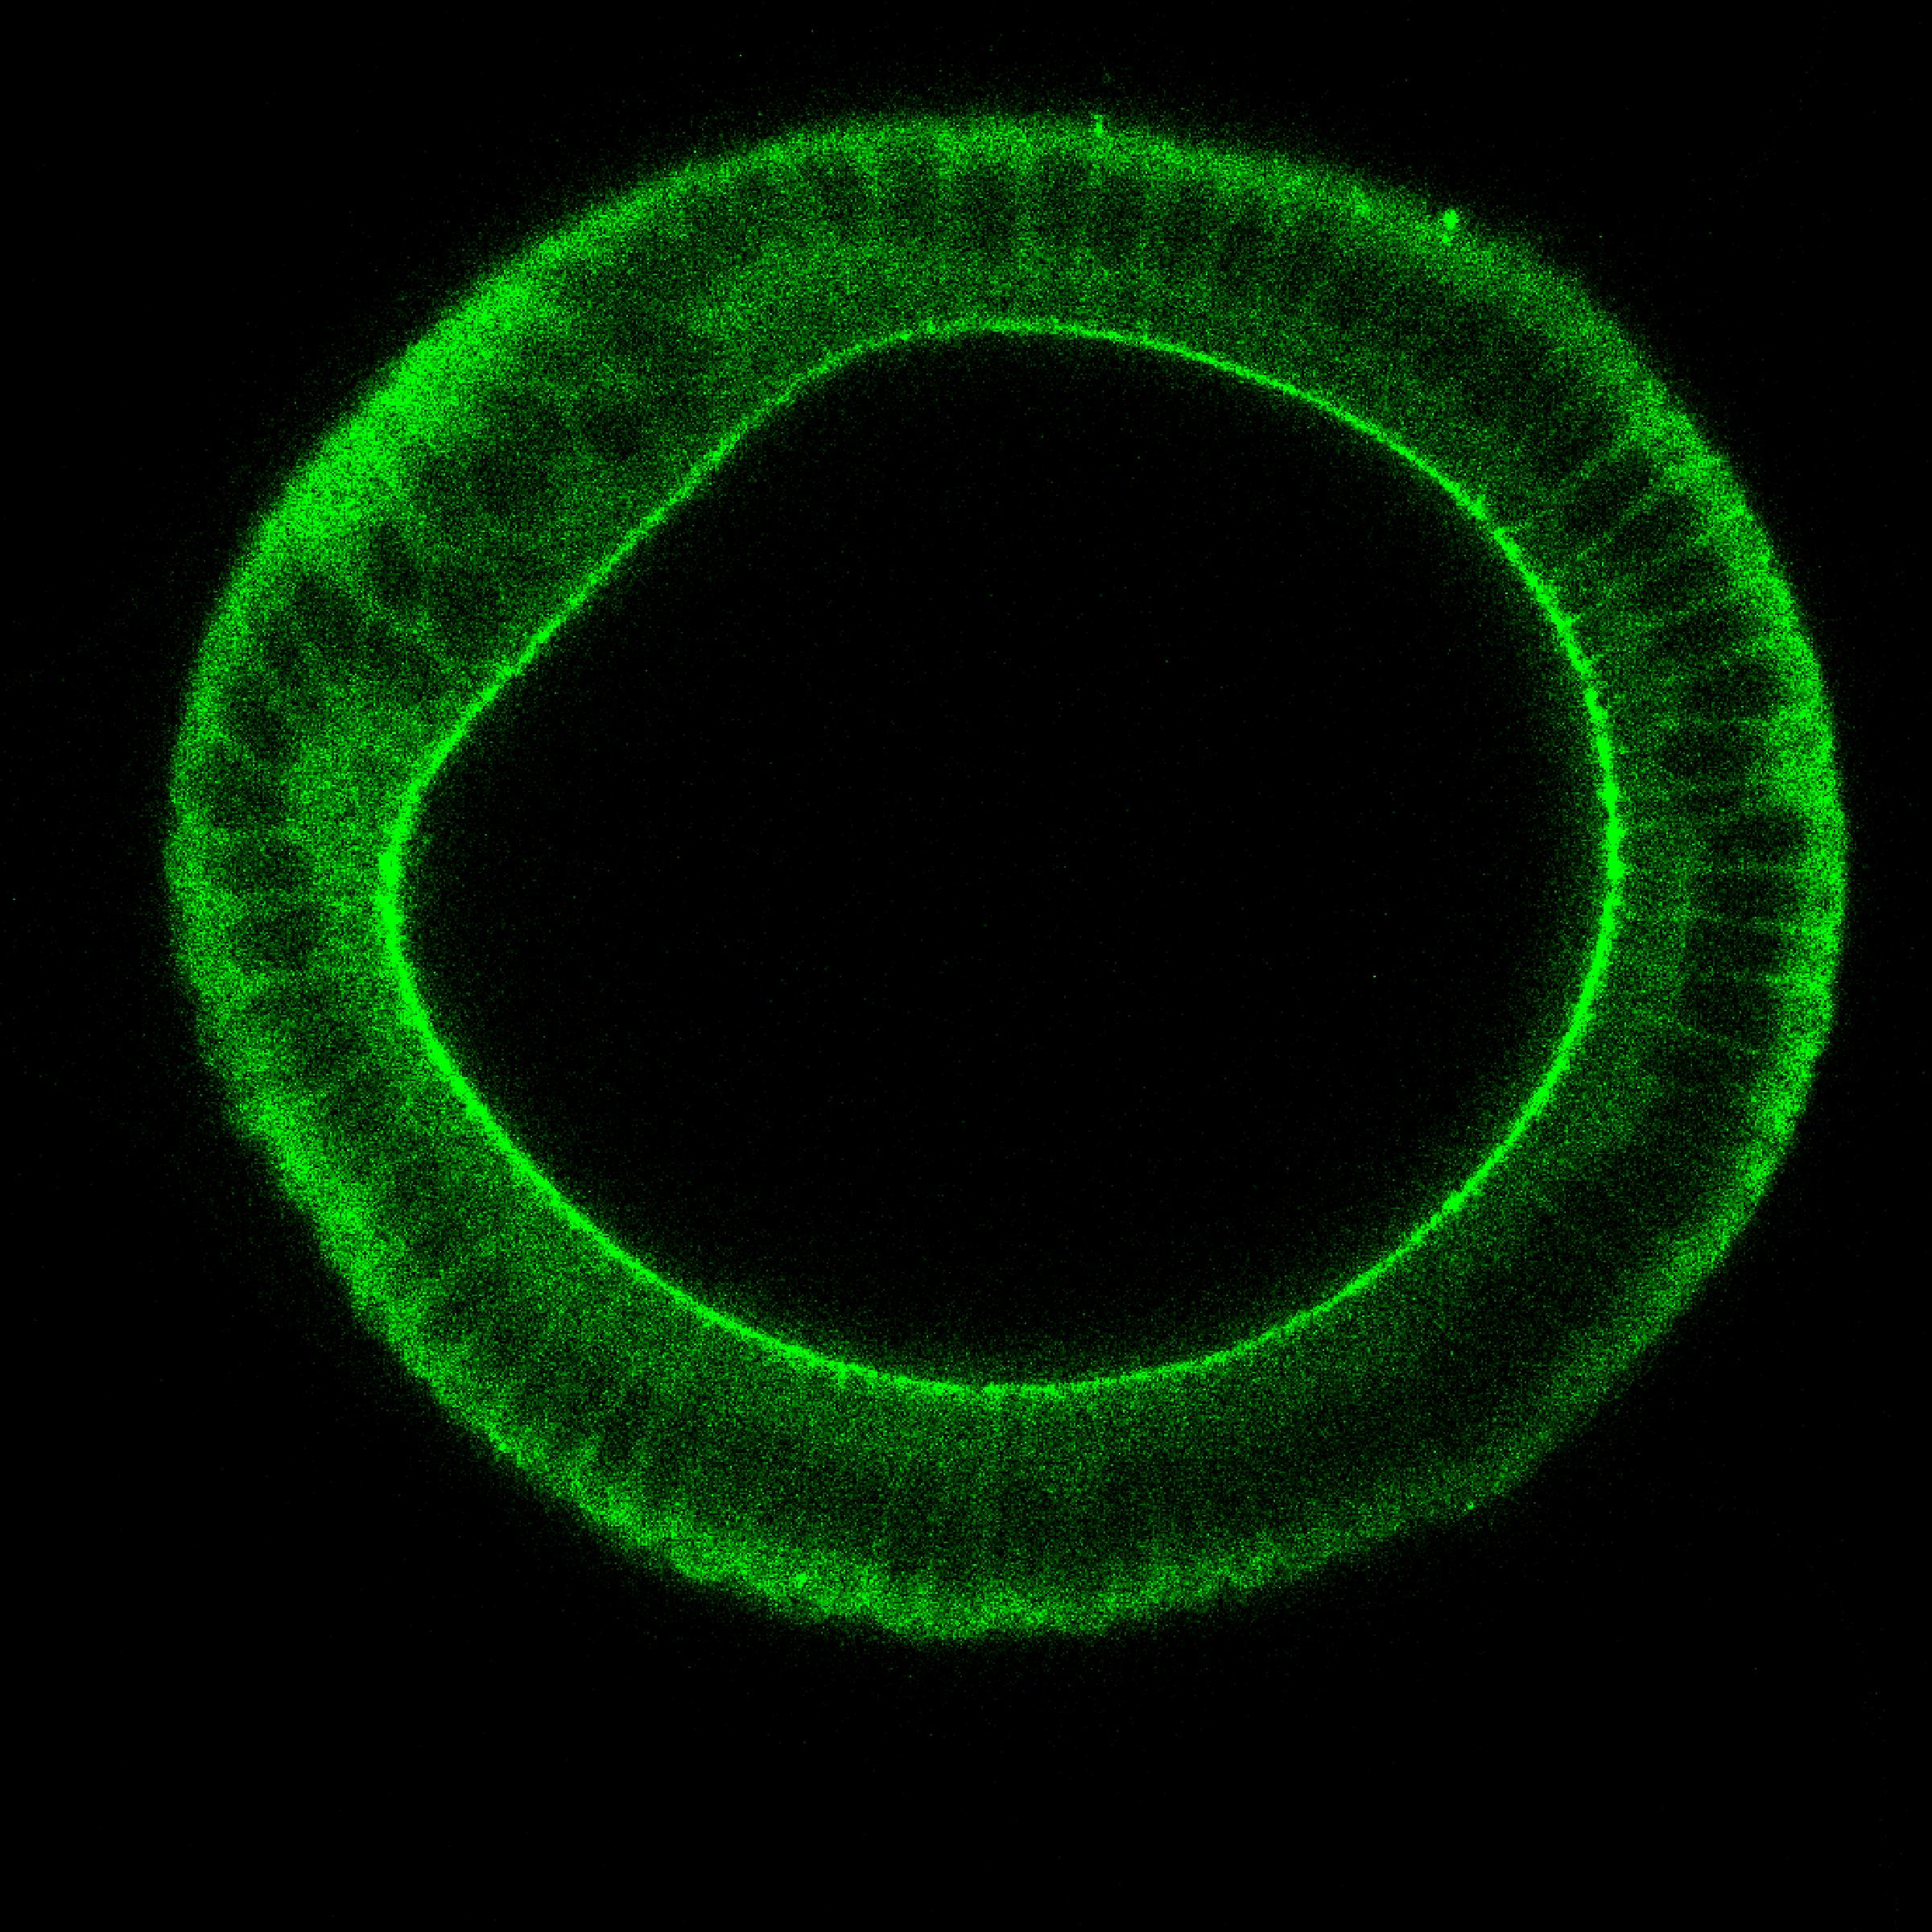
\includegraphics[width=0.3\textwidth]{drosophila_membrane}
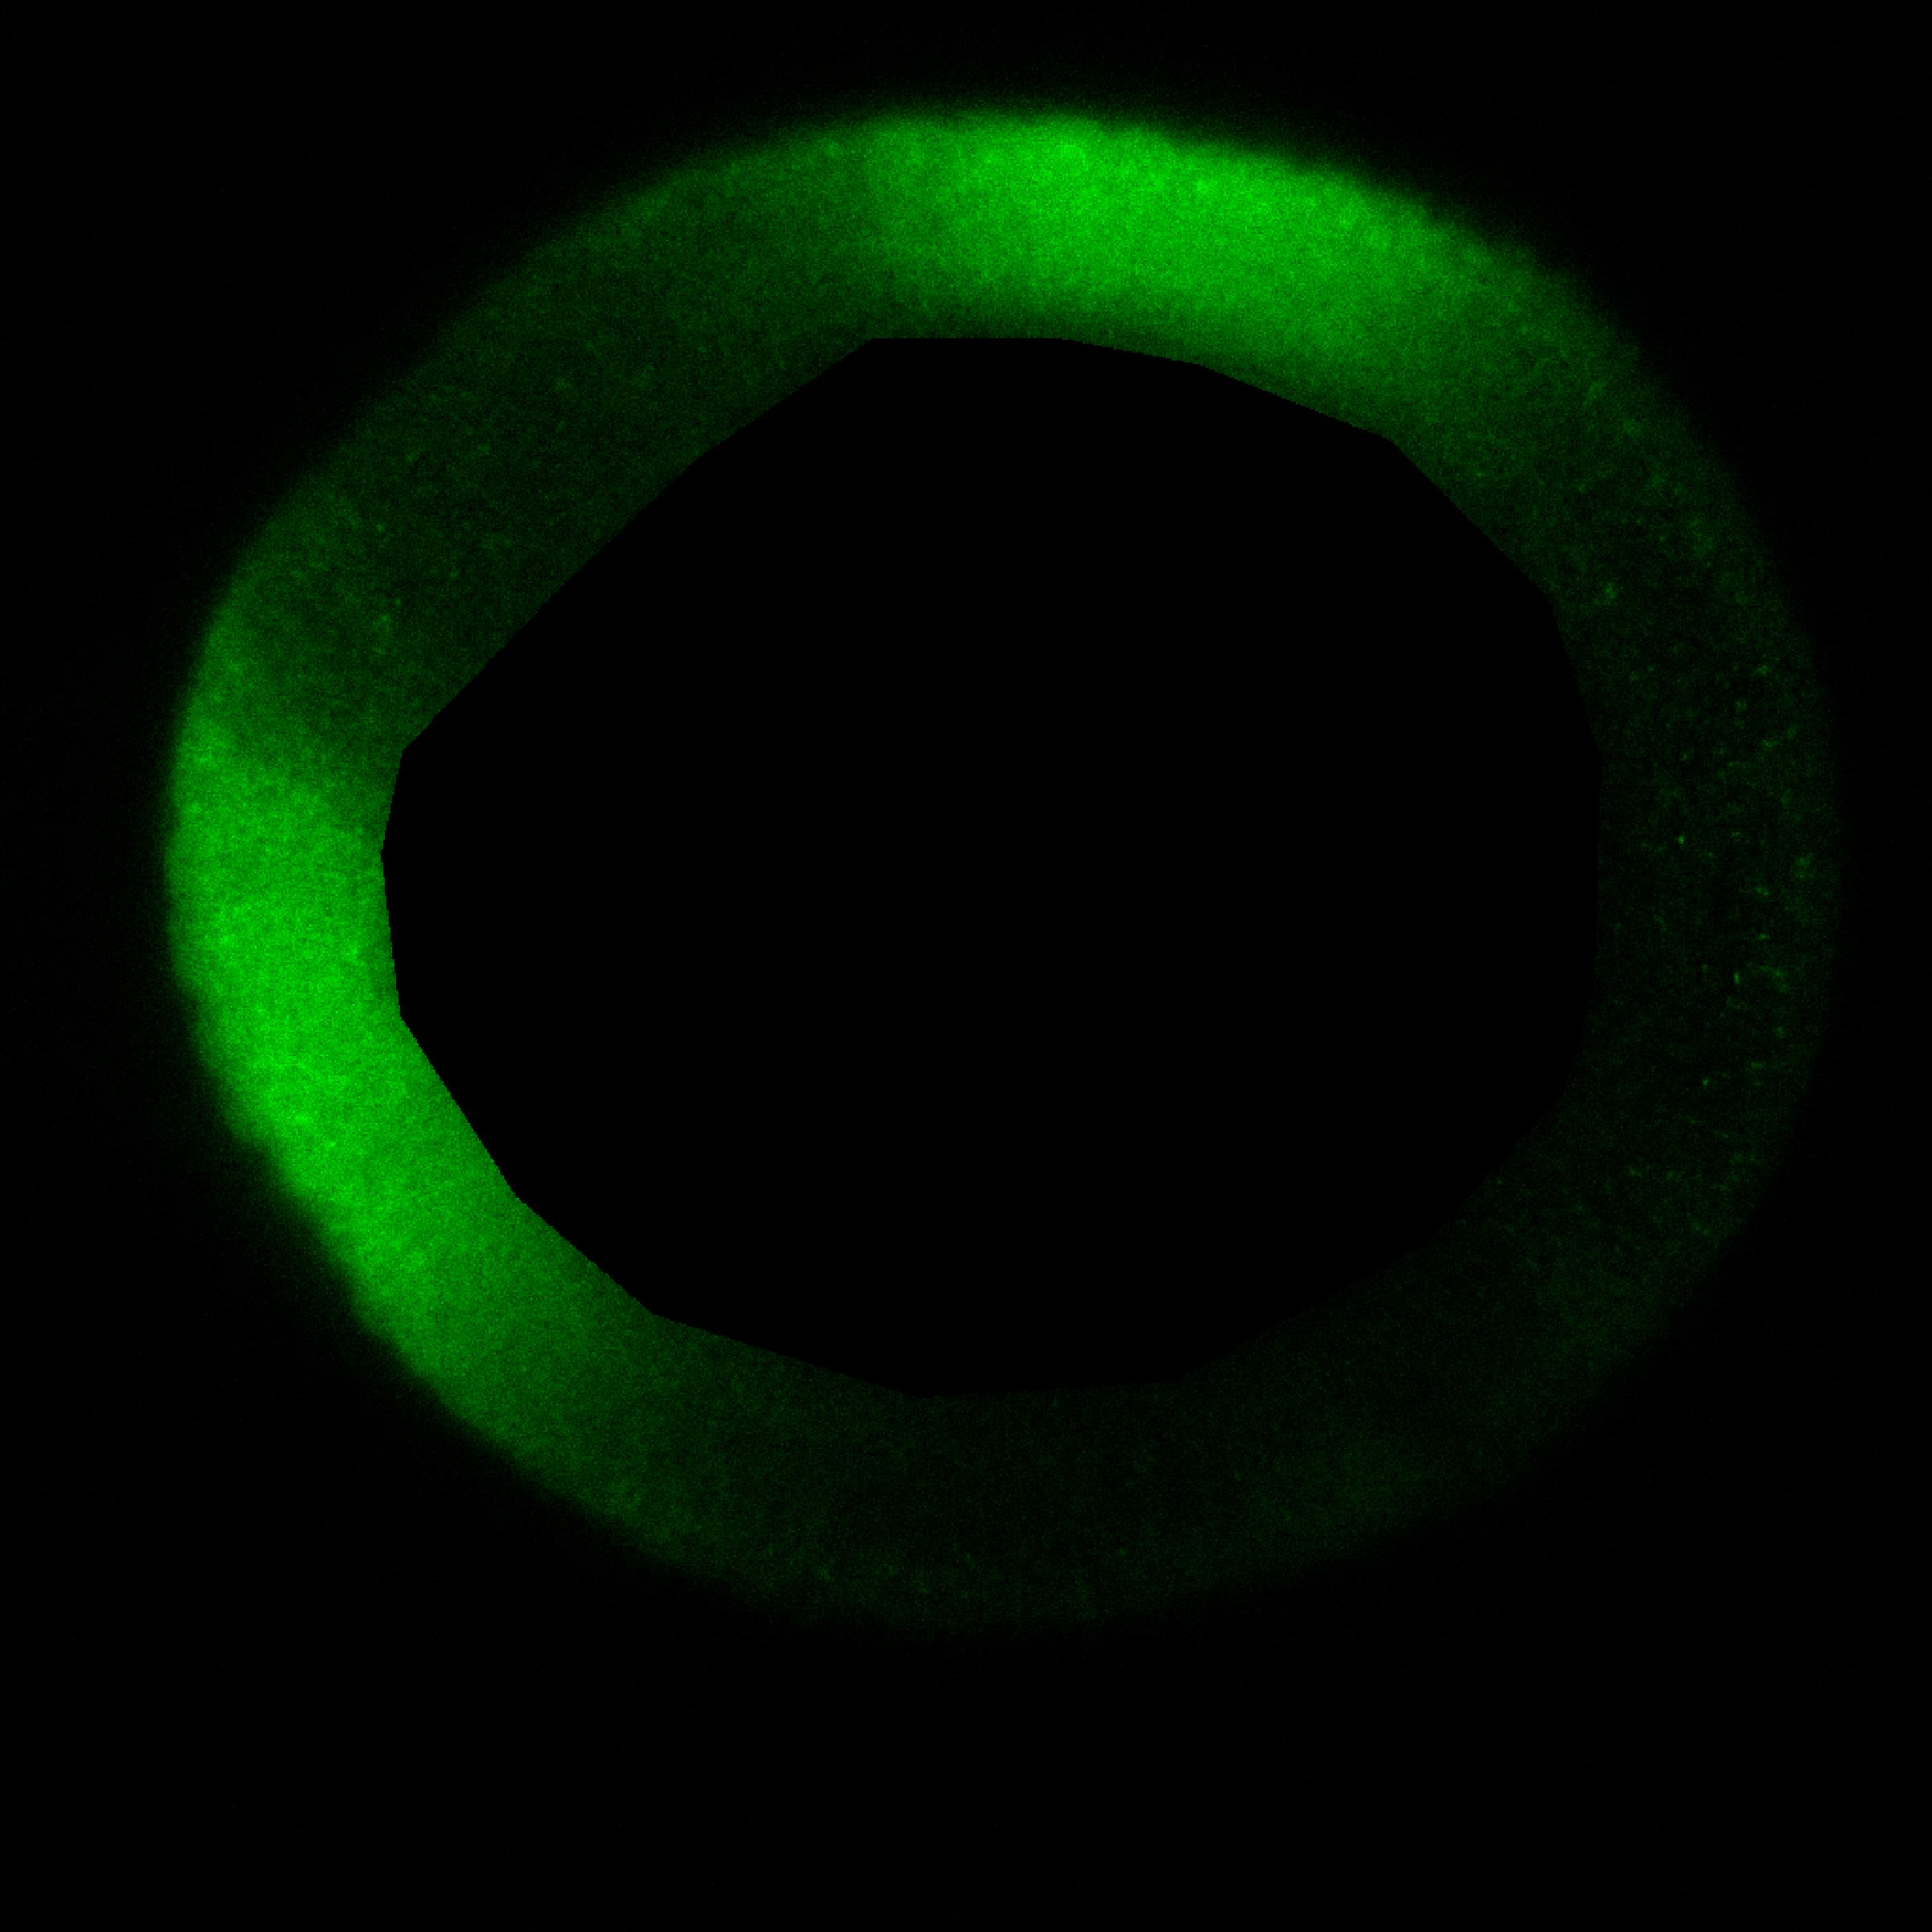
\includegraphics[width=0.3\textwidth]{drosophila_dpERK}
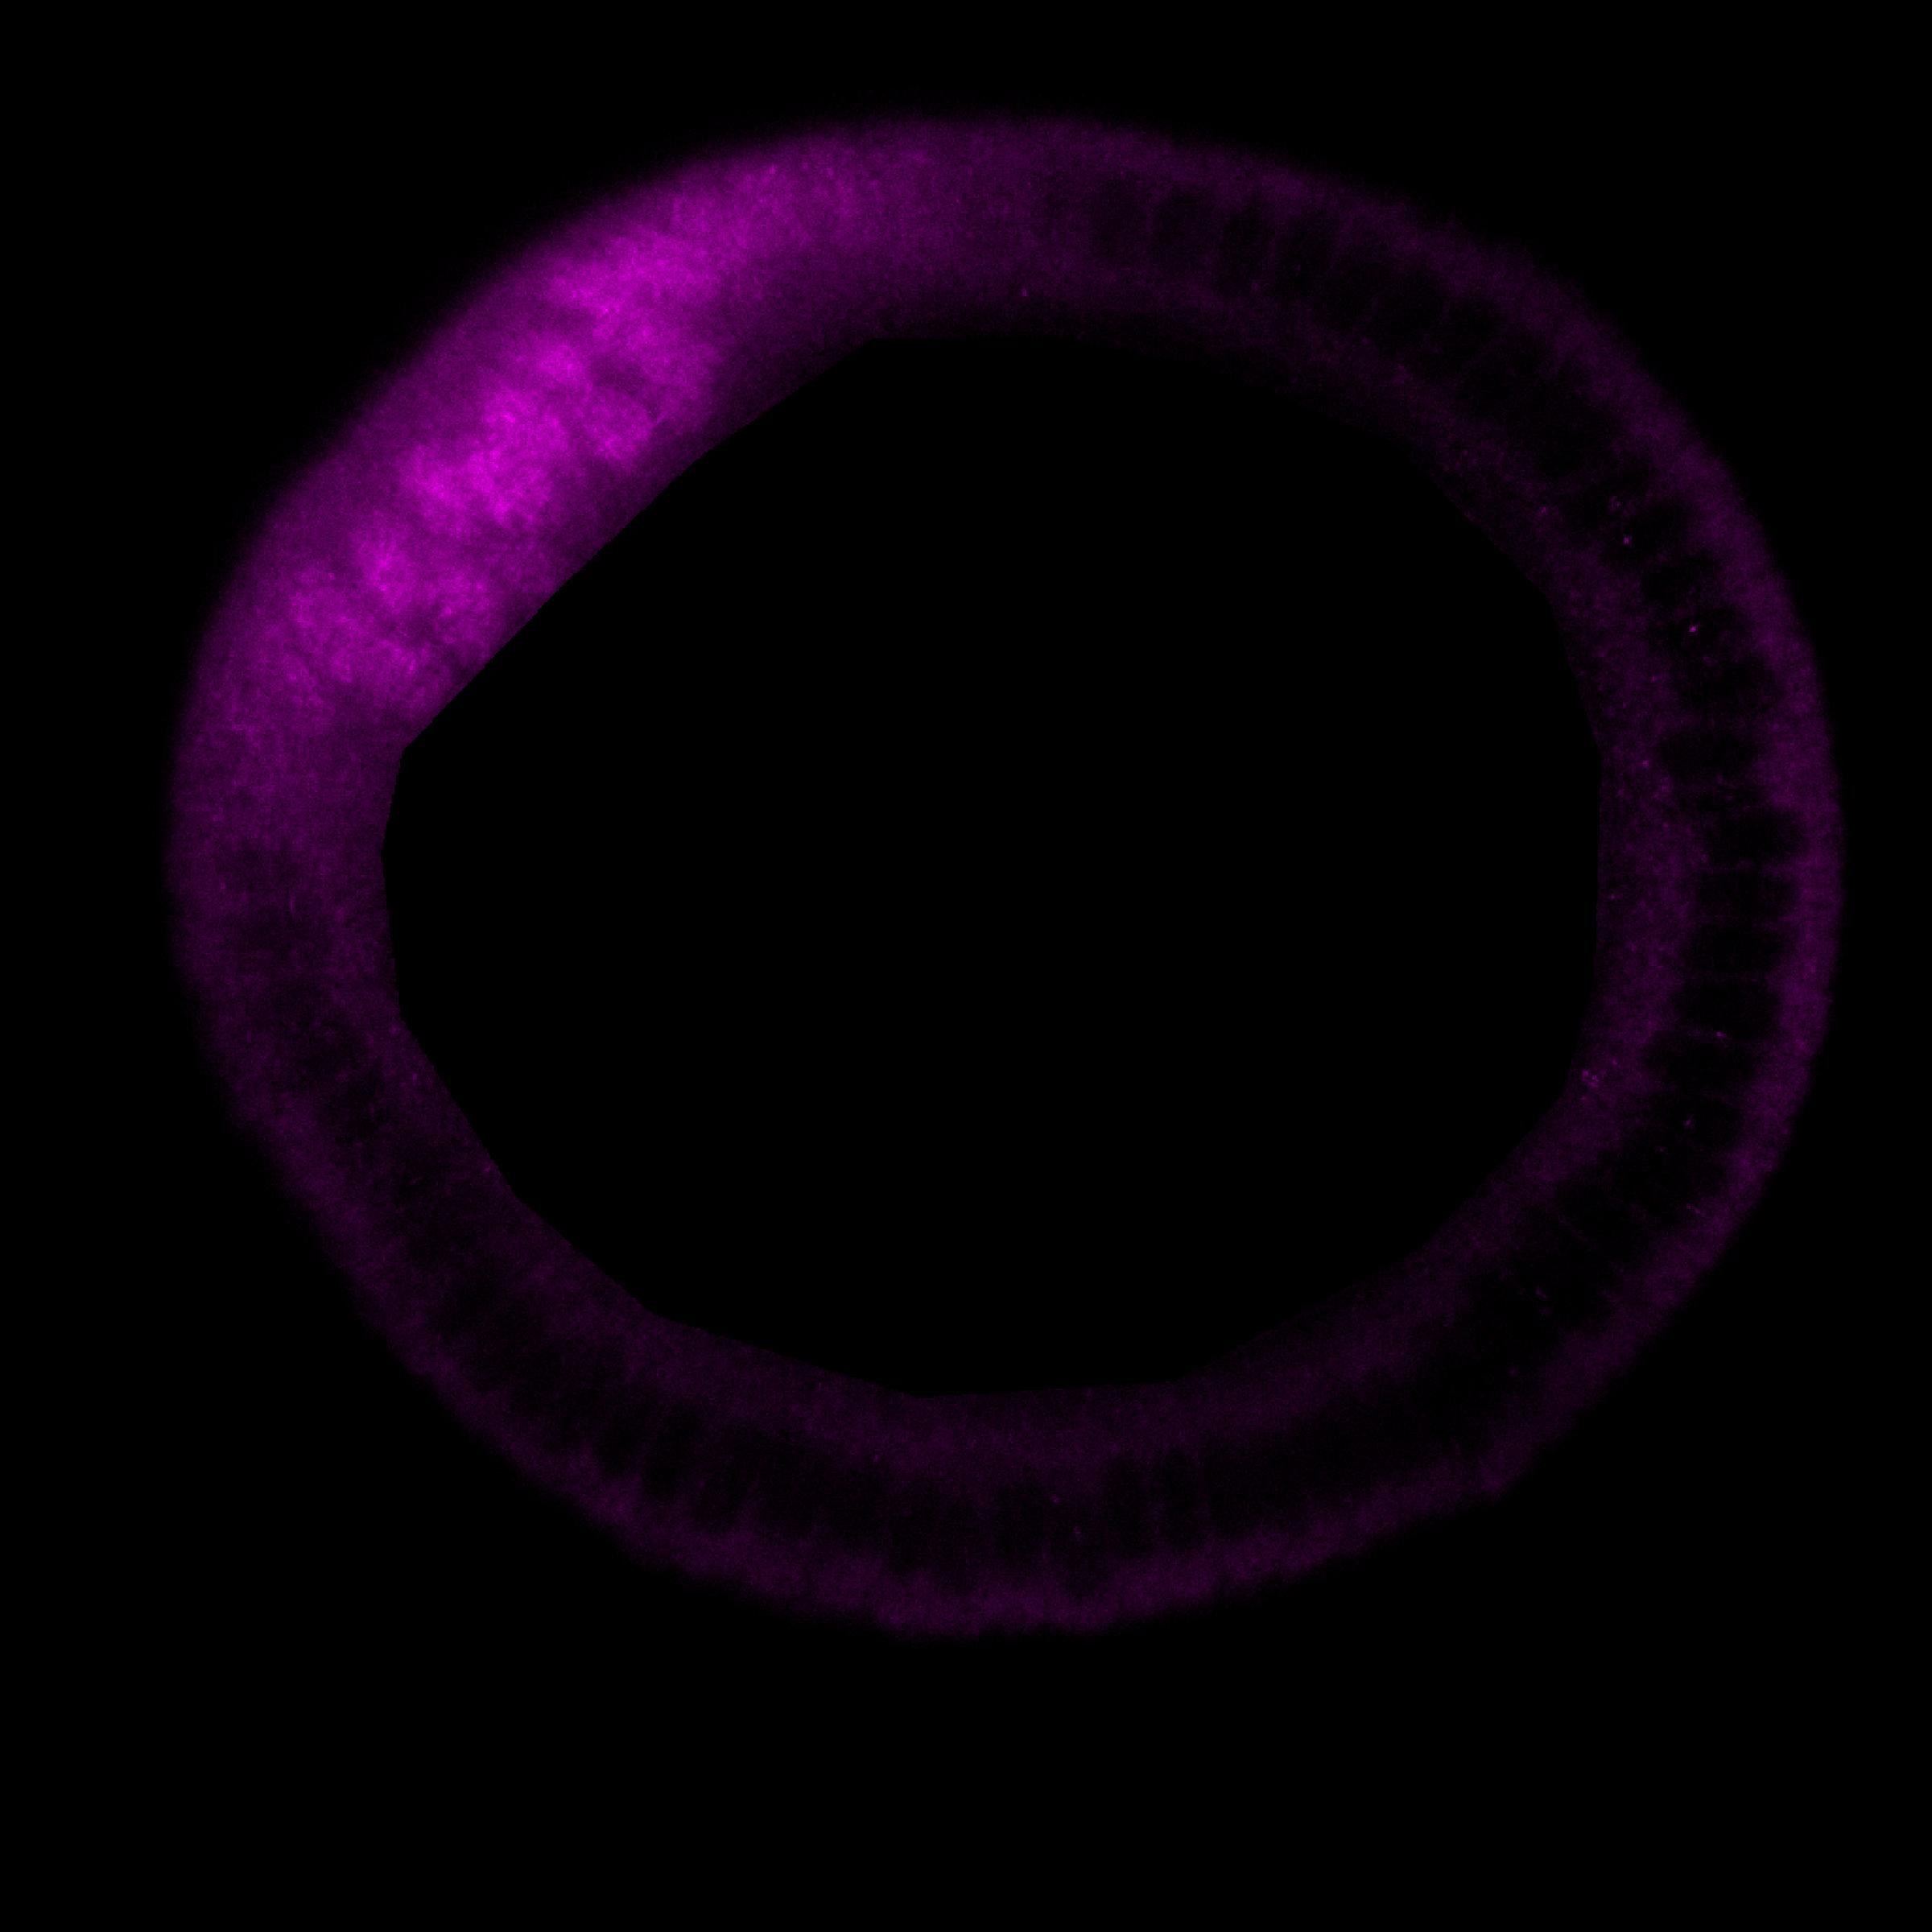
\includegraphics[width=0.3\textwidth]{drosophila_DI}
\caption{}
\end{subfigure}
\begin{subfigure}{0.35\textwidth}
\centering
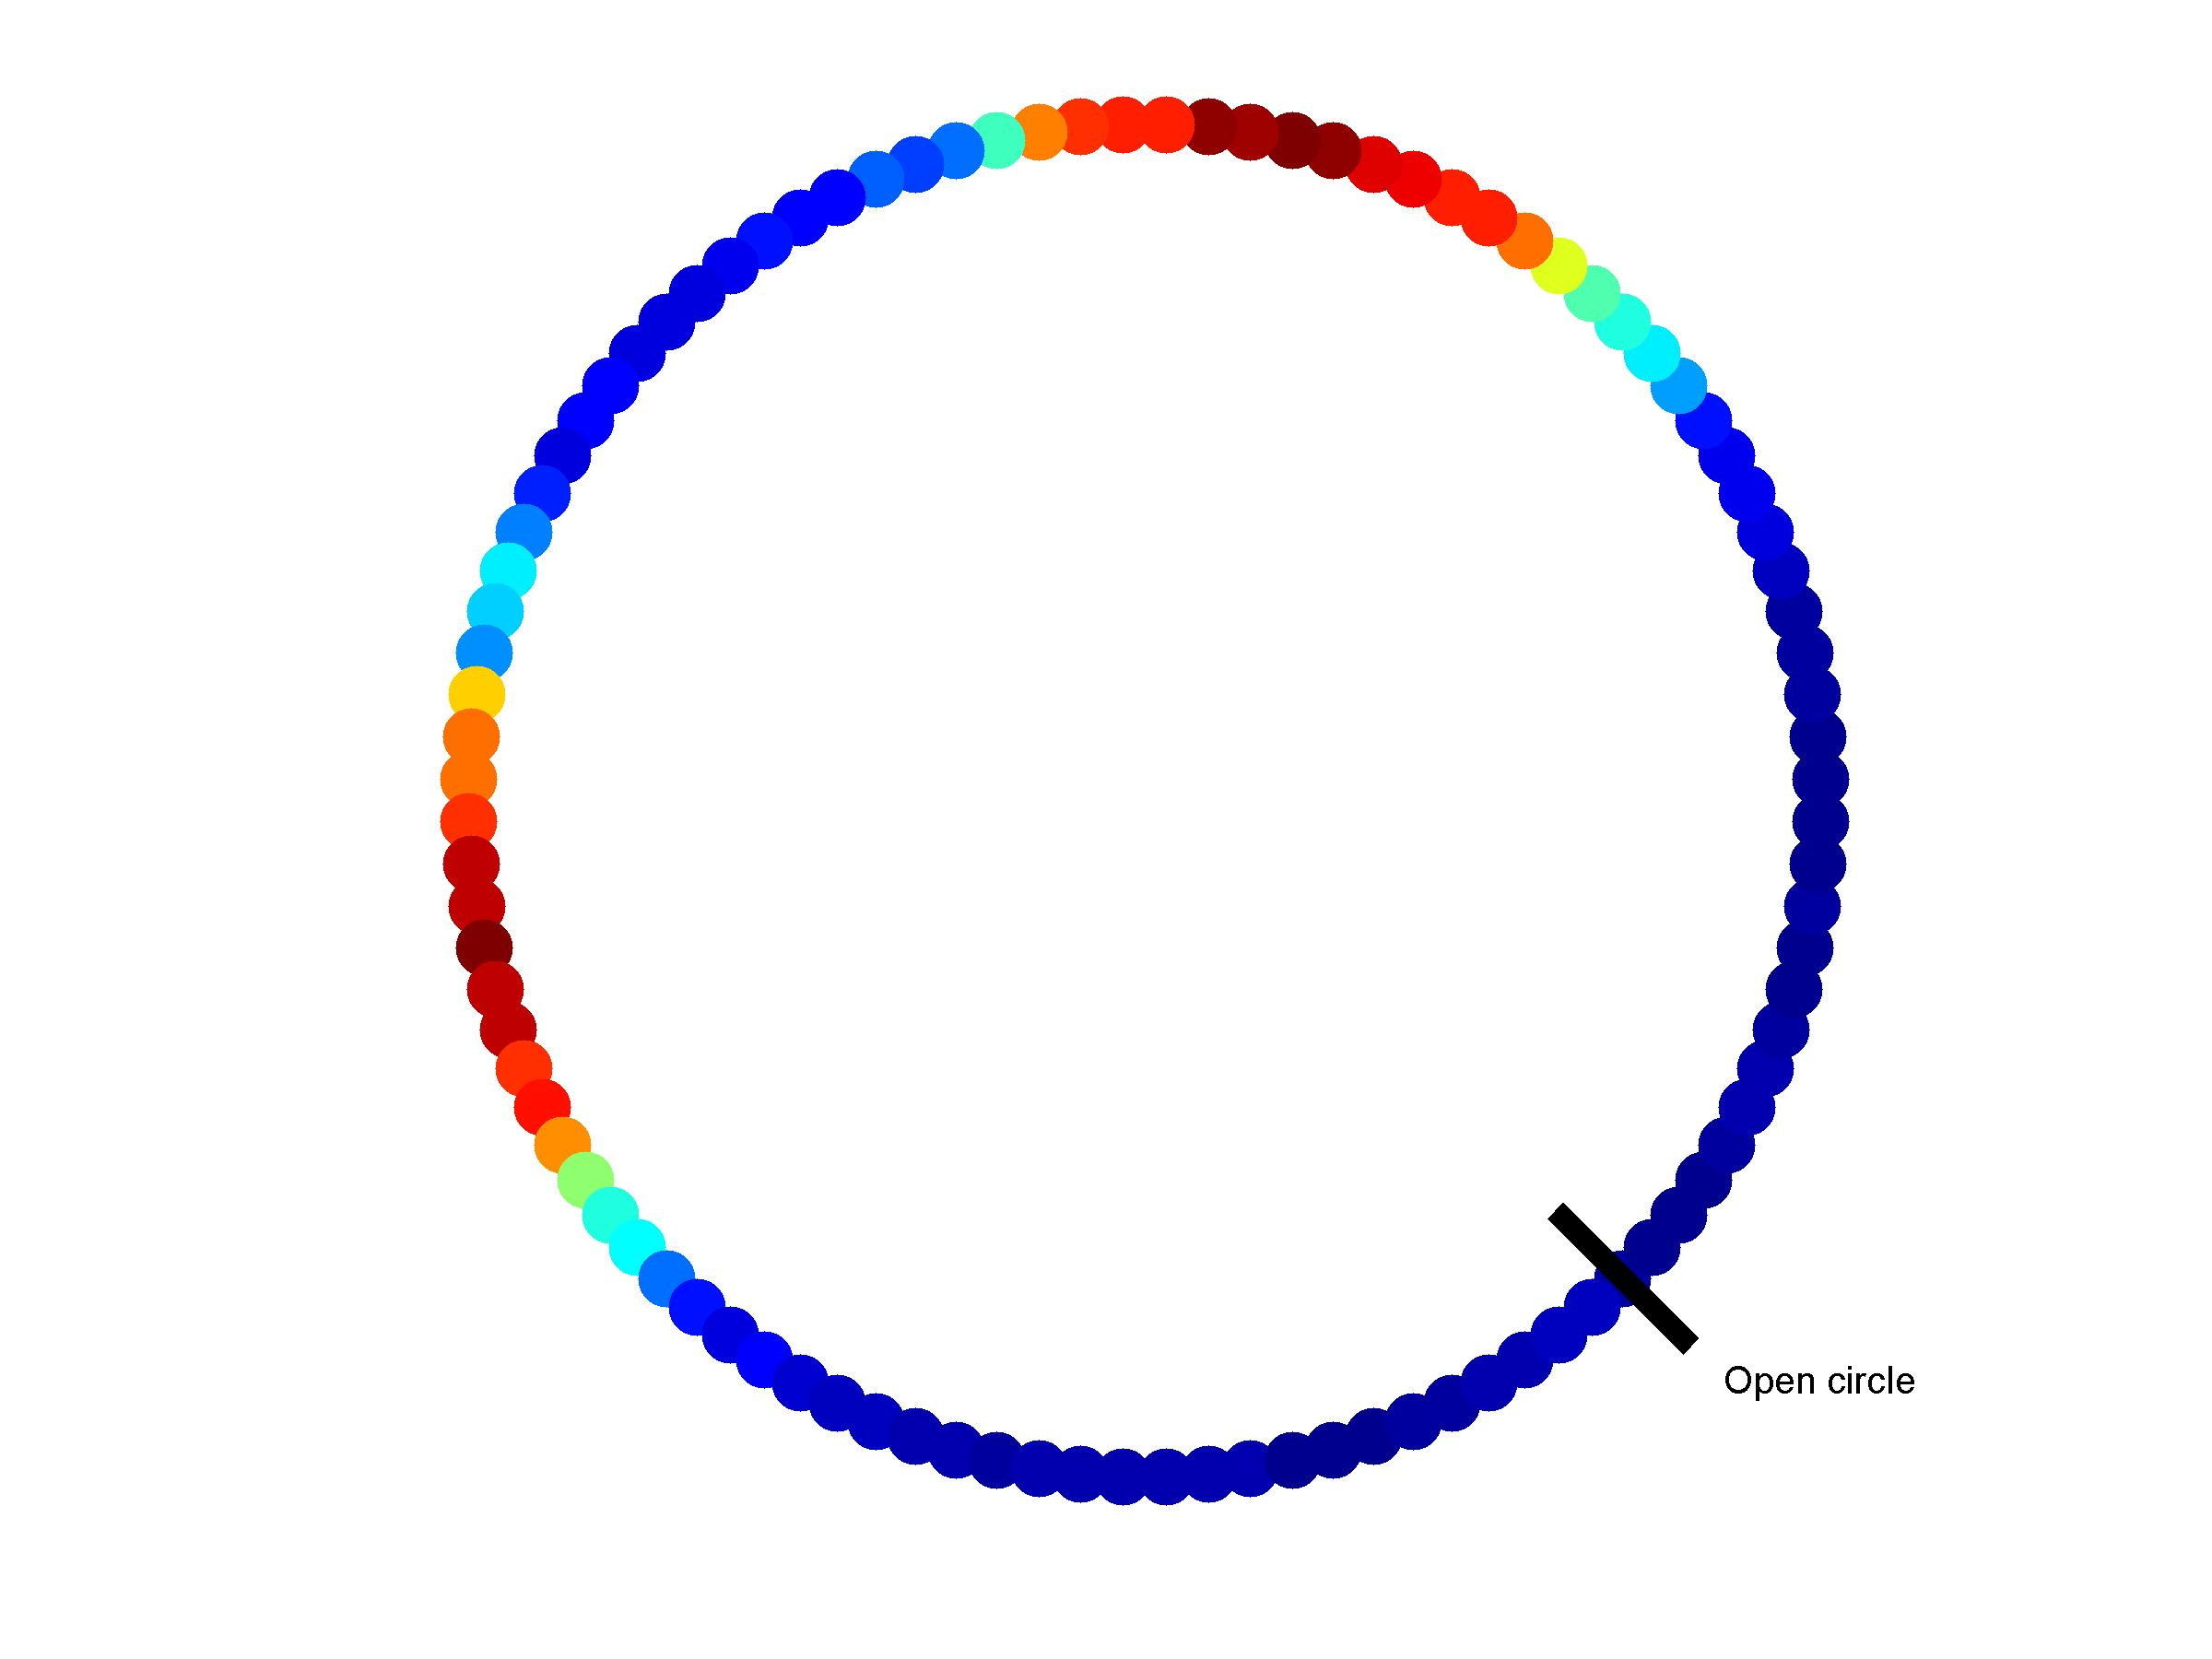
\includegraphics[width=0.6\textwidth]{circle_profile}\\
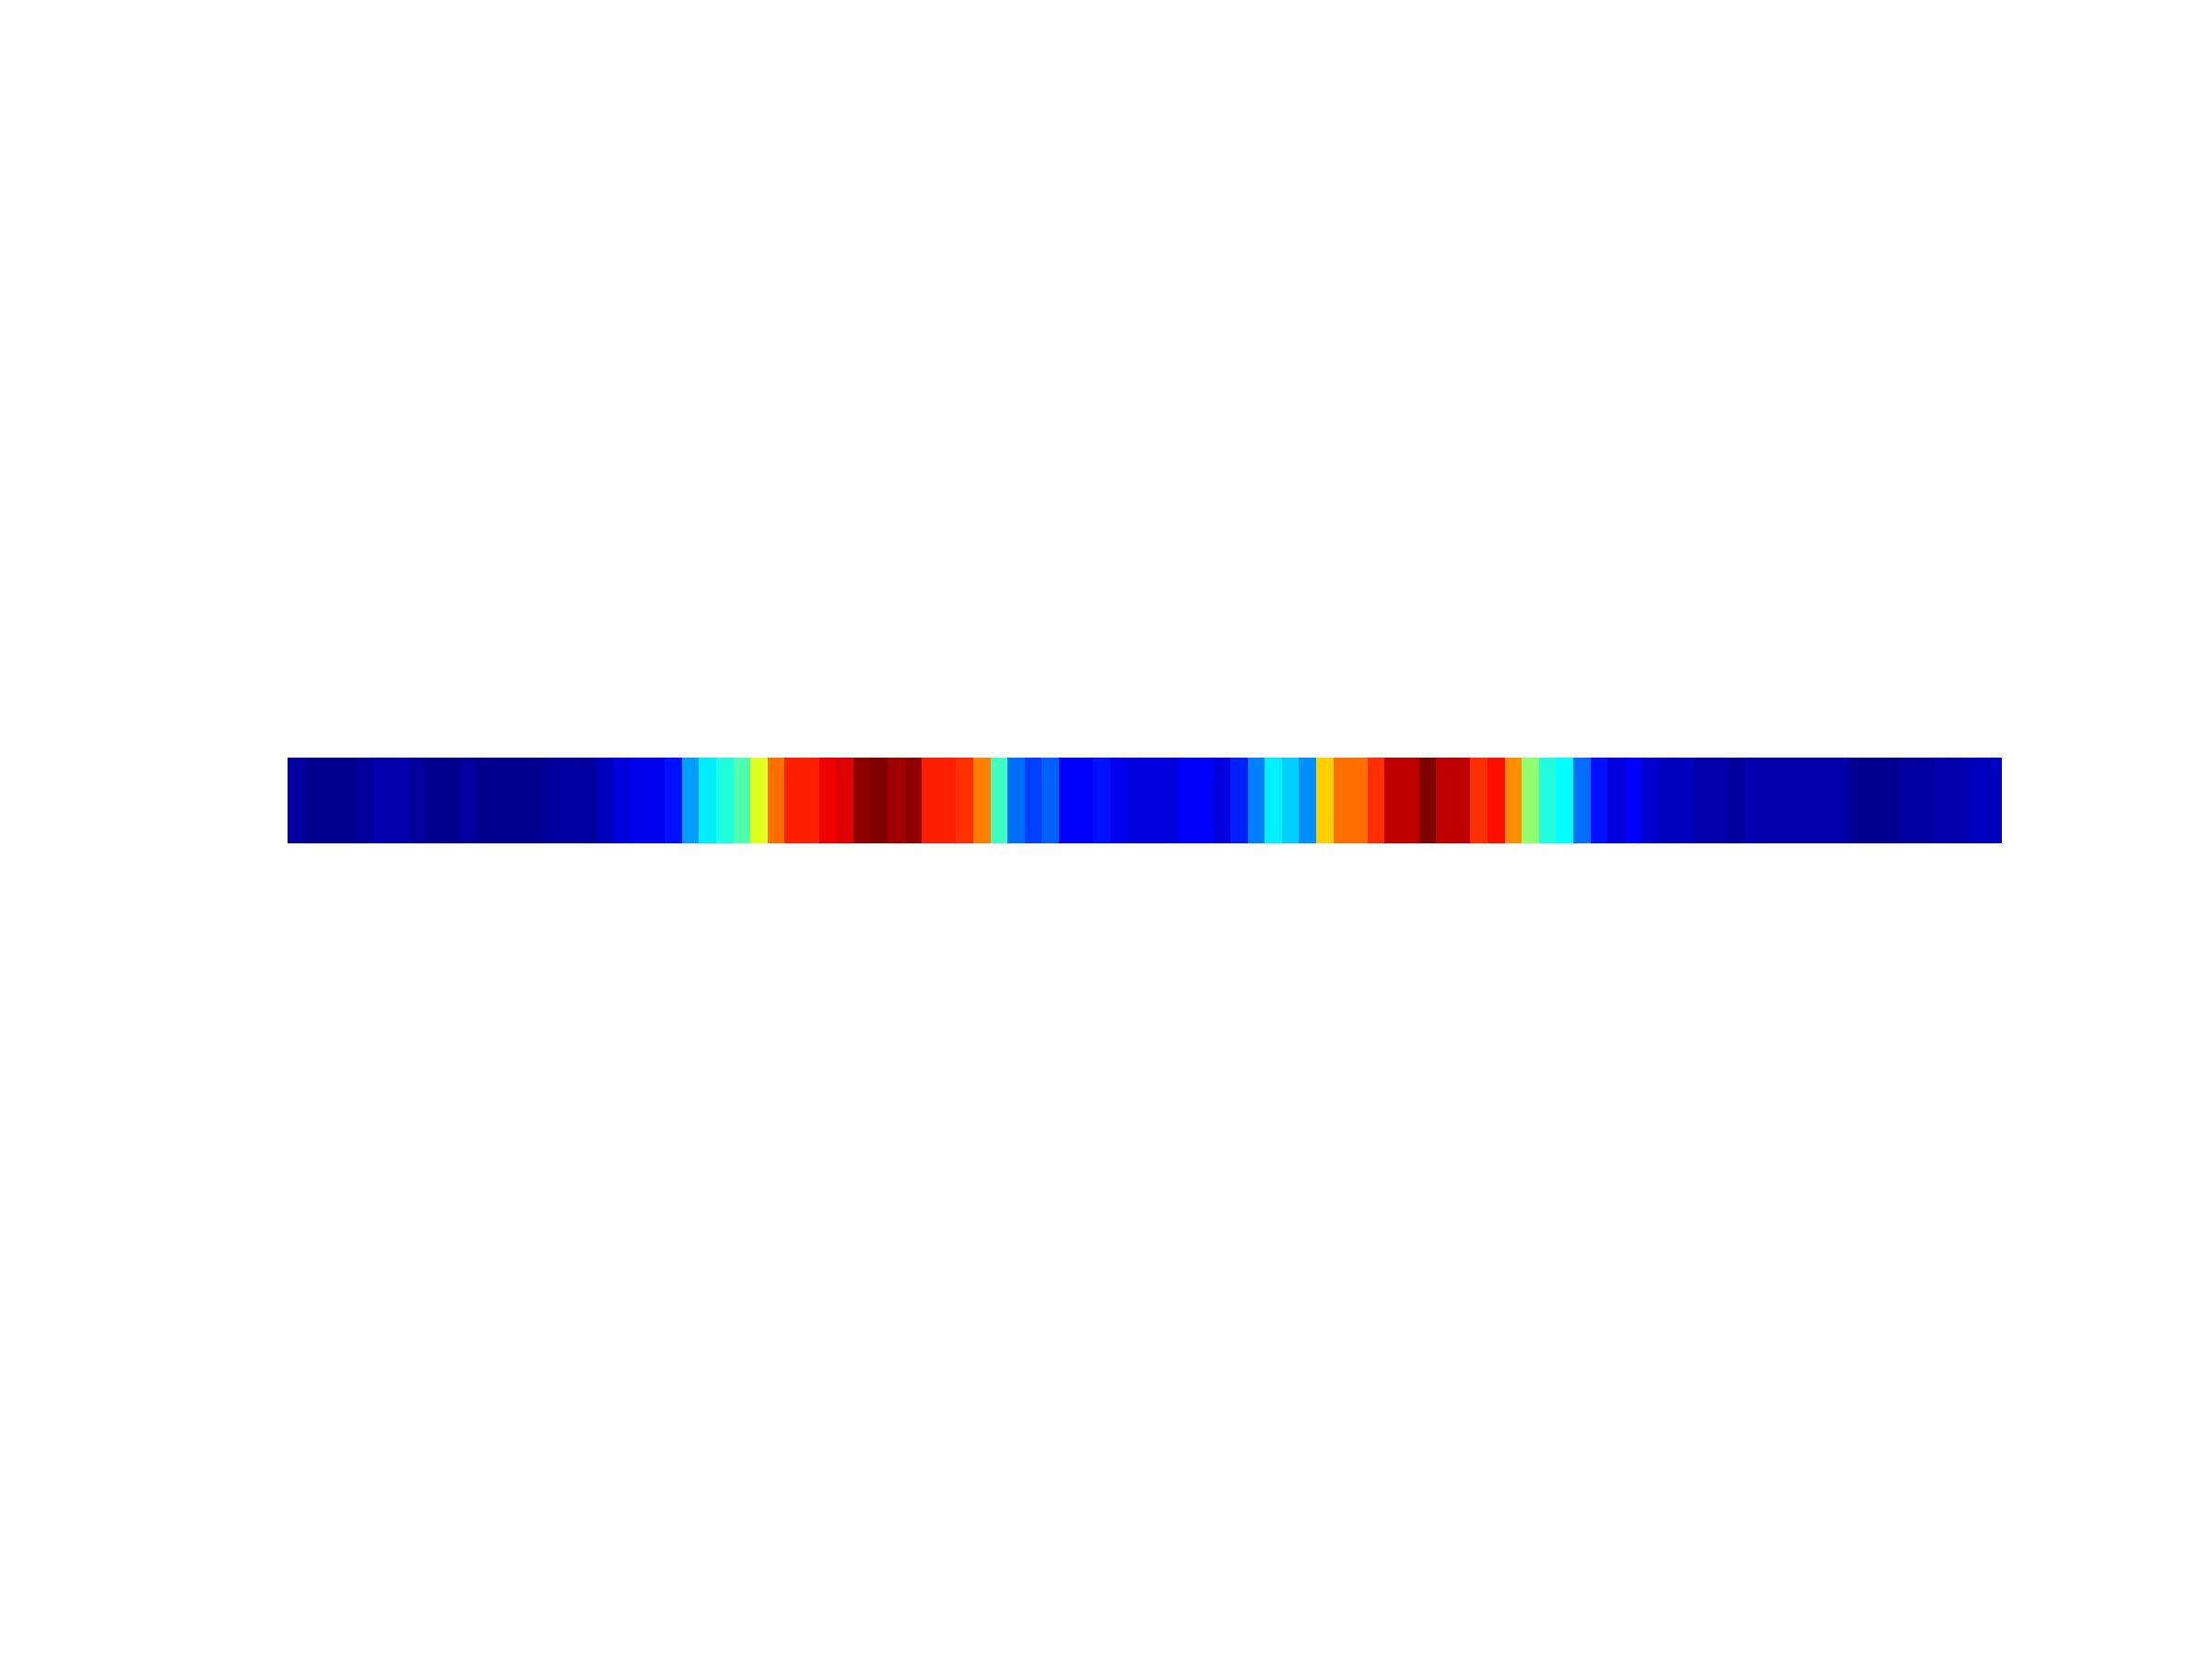
\includegraphics[width=\textwidth, trim=0mm 300mm 0mm 200mm, clip]{line_profile}
\caption{}
\end{subfigure}\\
\begin{subfigure}{0.45\textwidth}
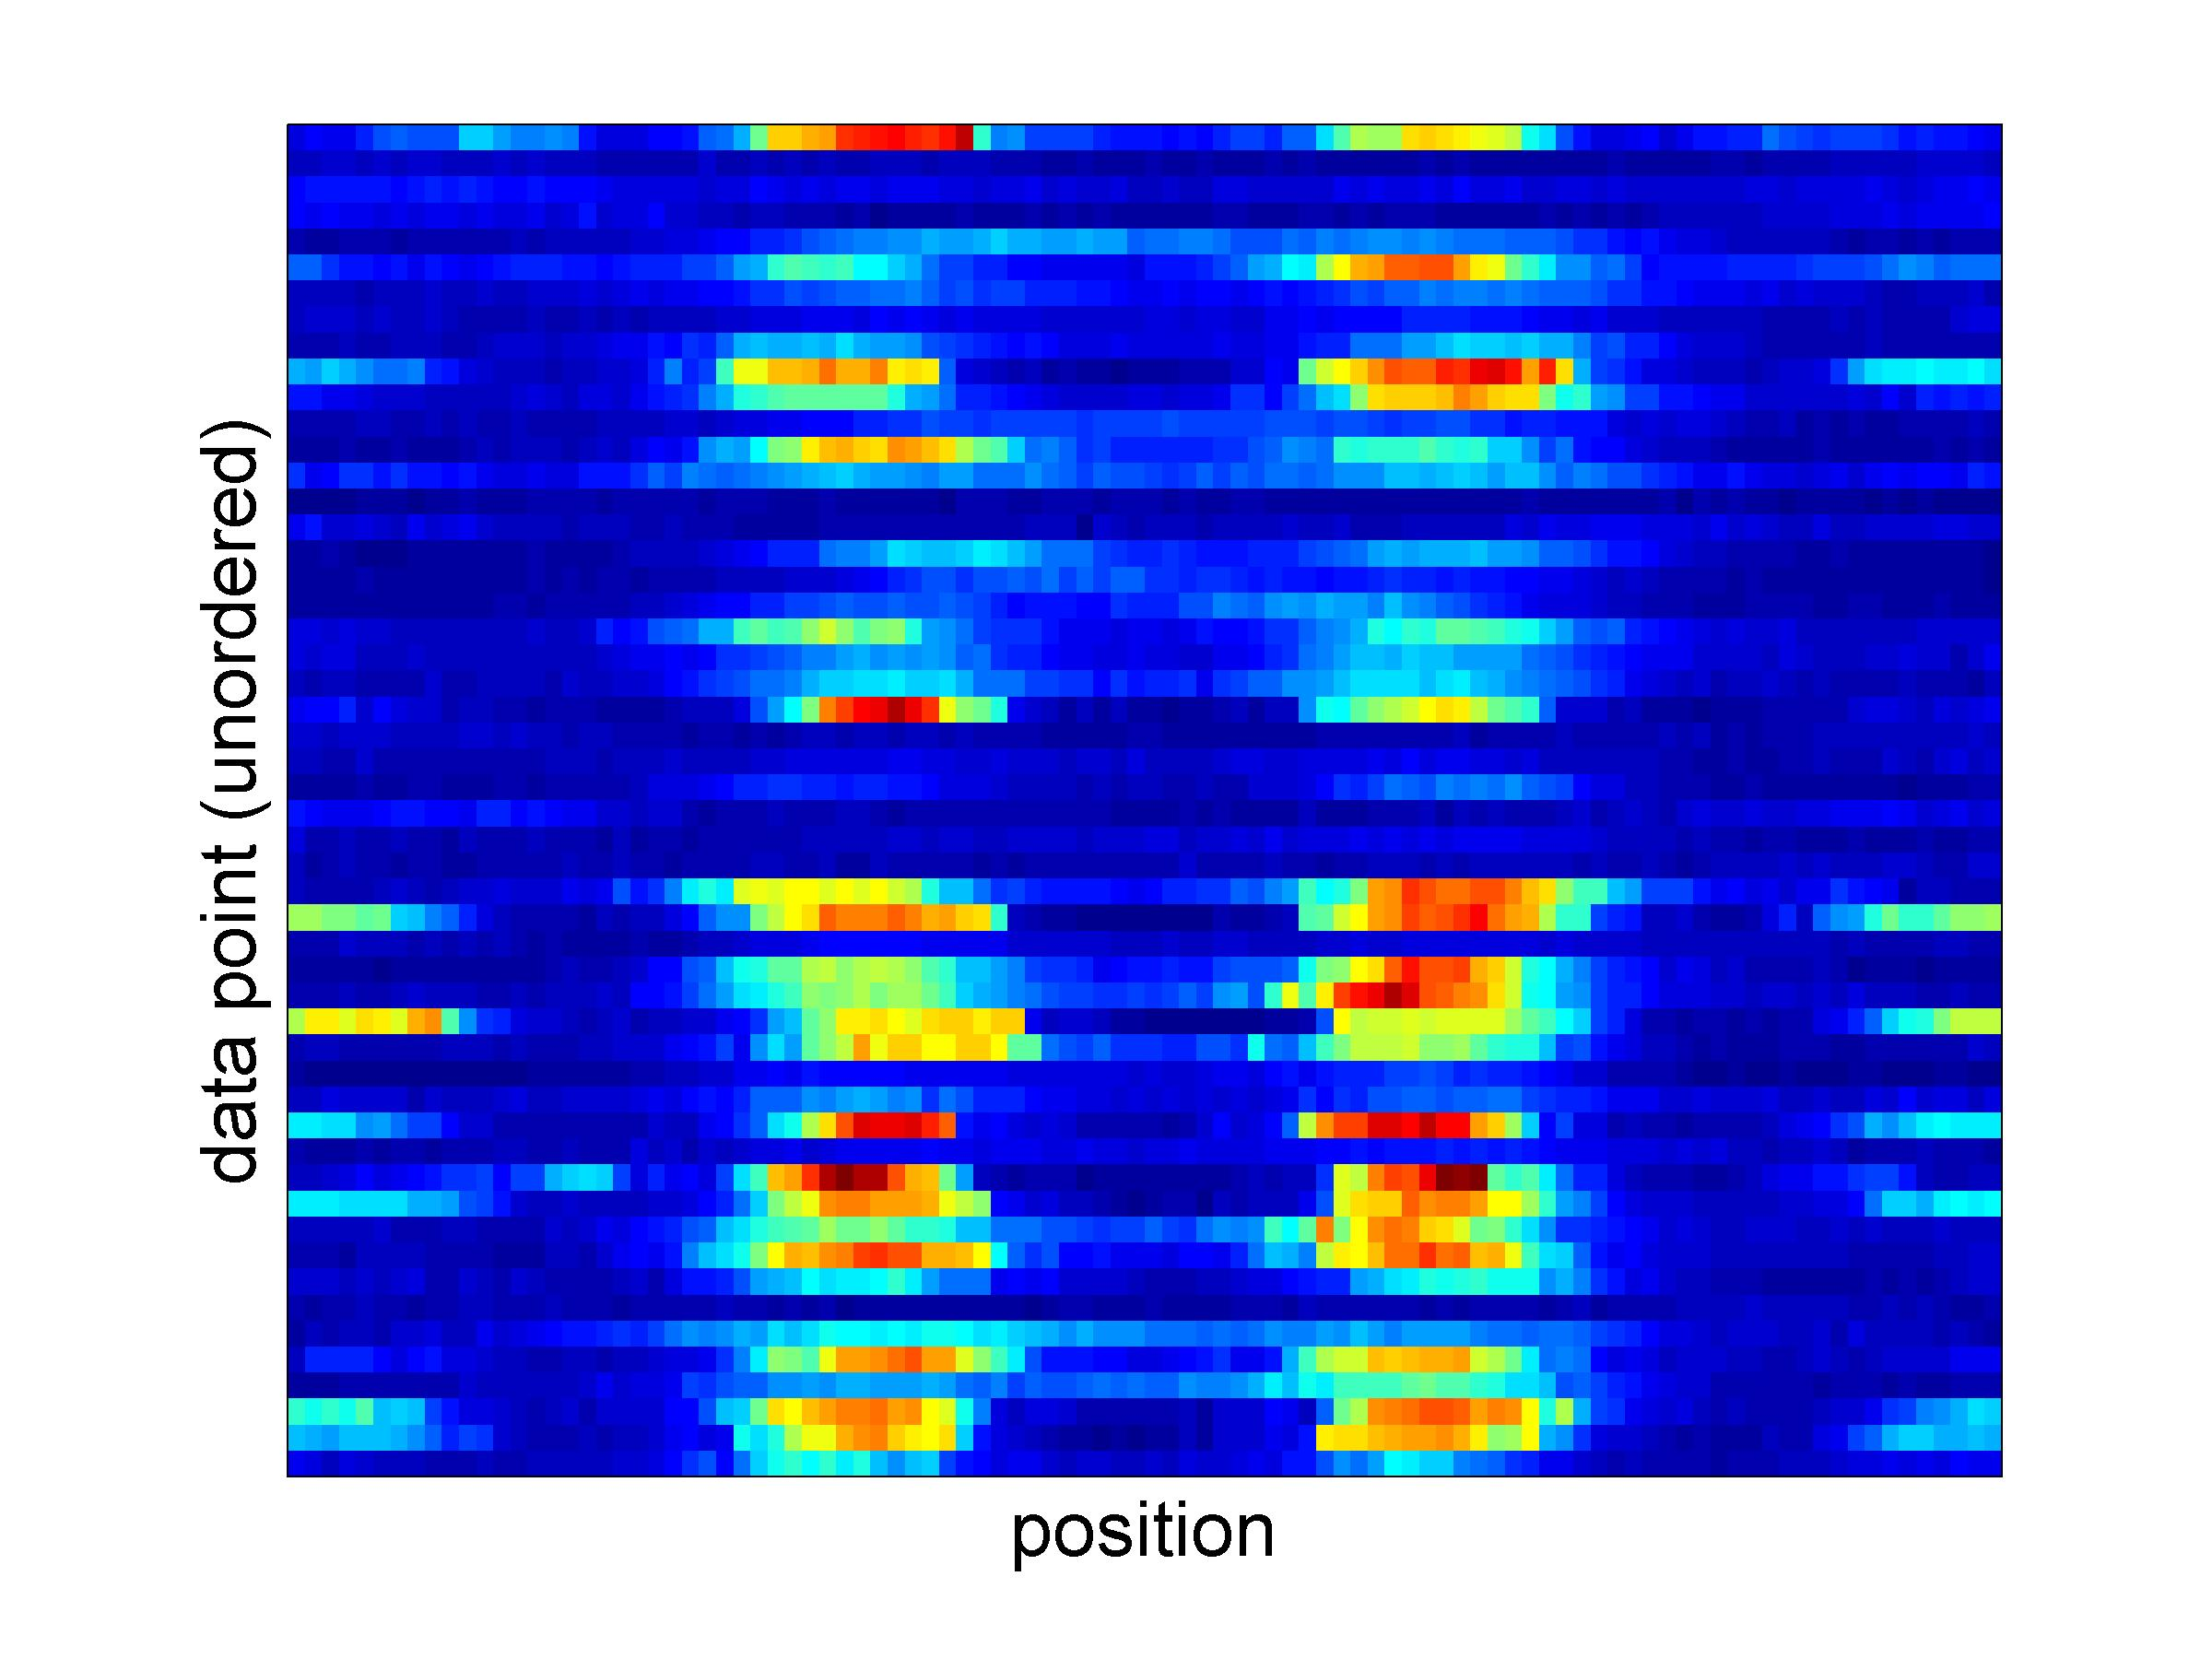
\includegraphics[width=\textwidth]{data_unordered}
\caption{}
\end{subfigure}
\begin{subfigure}{0.45\textwidth}
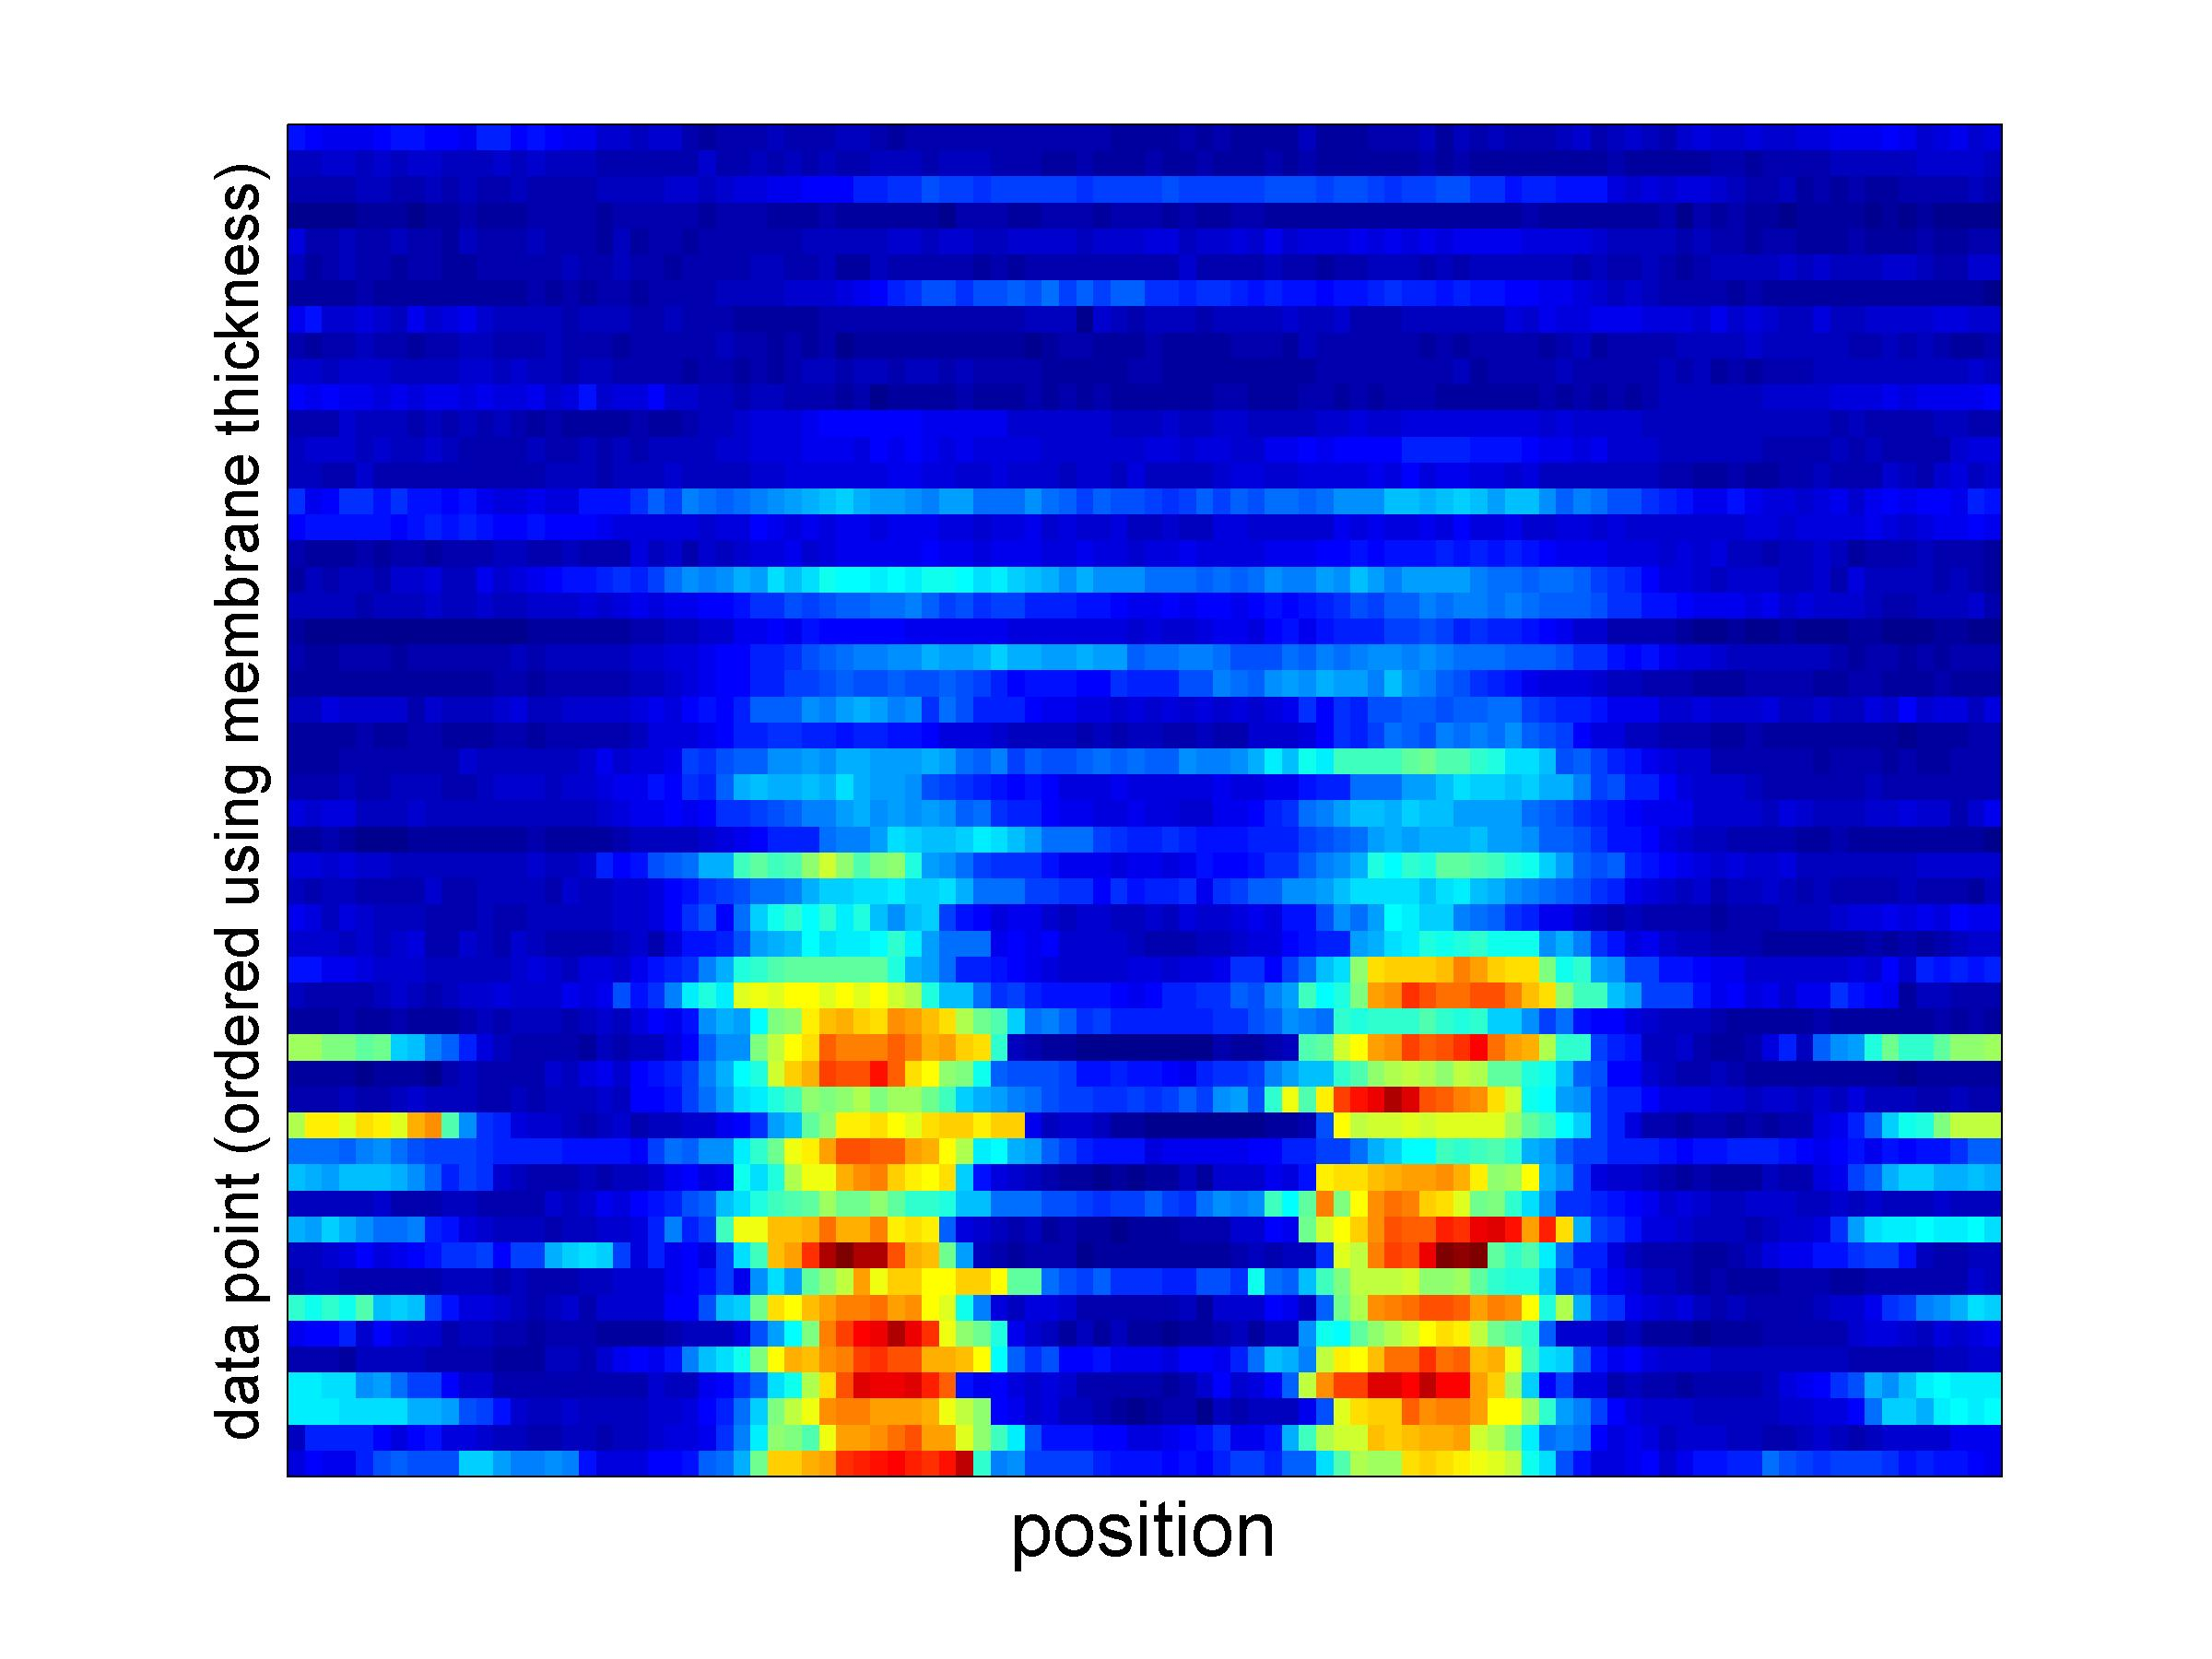
\includegraphics[width=\textwidth]{data_ordered_membrane}
\caption{}
\end{subfigure}
\end{center}
\caption{{\bf Data collection.} (a) Schematic of {\em Drosophila} embryo (longitudinal and cross-section), and cross-sectional fluorescent images of an embryo stained for the membrane proteins (left), dpERK (center), and dorsal protein (right).
(b) Concentration profile of dpERK extracted from a fluorescent image. The circular profile is ``unwrapped'' at the dorsal midline (determined from the expression of the dorsal protein) to obtain a concentration profile on a line.
(c) Concentration profiles of dpERK for many embryos. Each row represents a different embryo fixed at a slightly different developmental time.
(d) Concentration profiles of dpERK for many embryos from (c), now ordered by the thickness of the membrane. The membrane thickness is known to be one-to-one with time.}
\label{fig:background}
\end{figure}

% Results and Discussion can be combined.
\section*{Results}

\subsection*{dpERK concentration profiles ordered using Principal Component Analysis}
\begin{figure}[H]
\begin{subfigure}{0.3\textwidth}
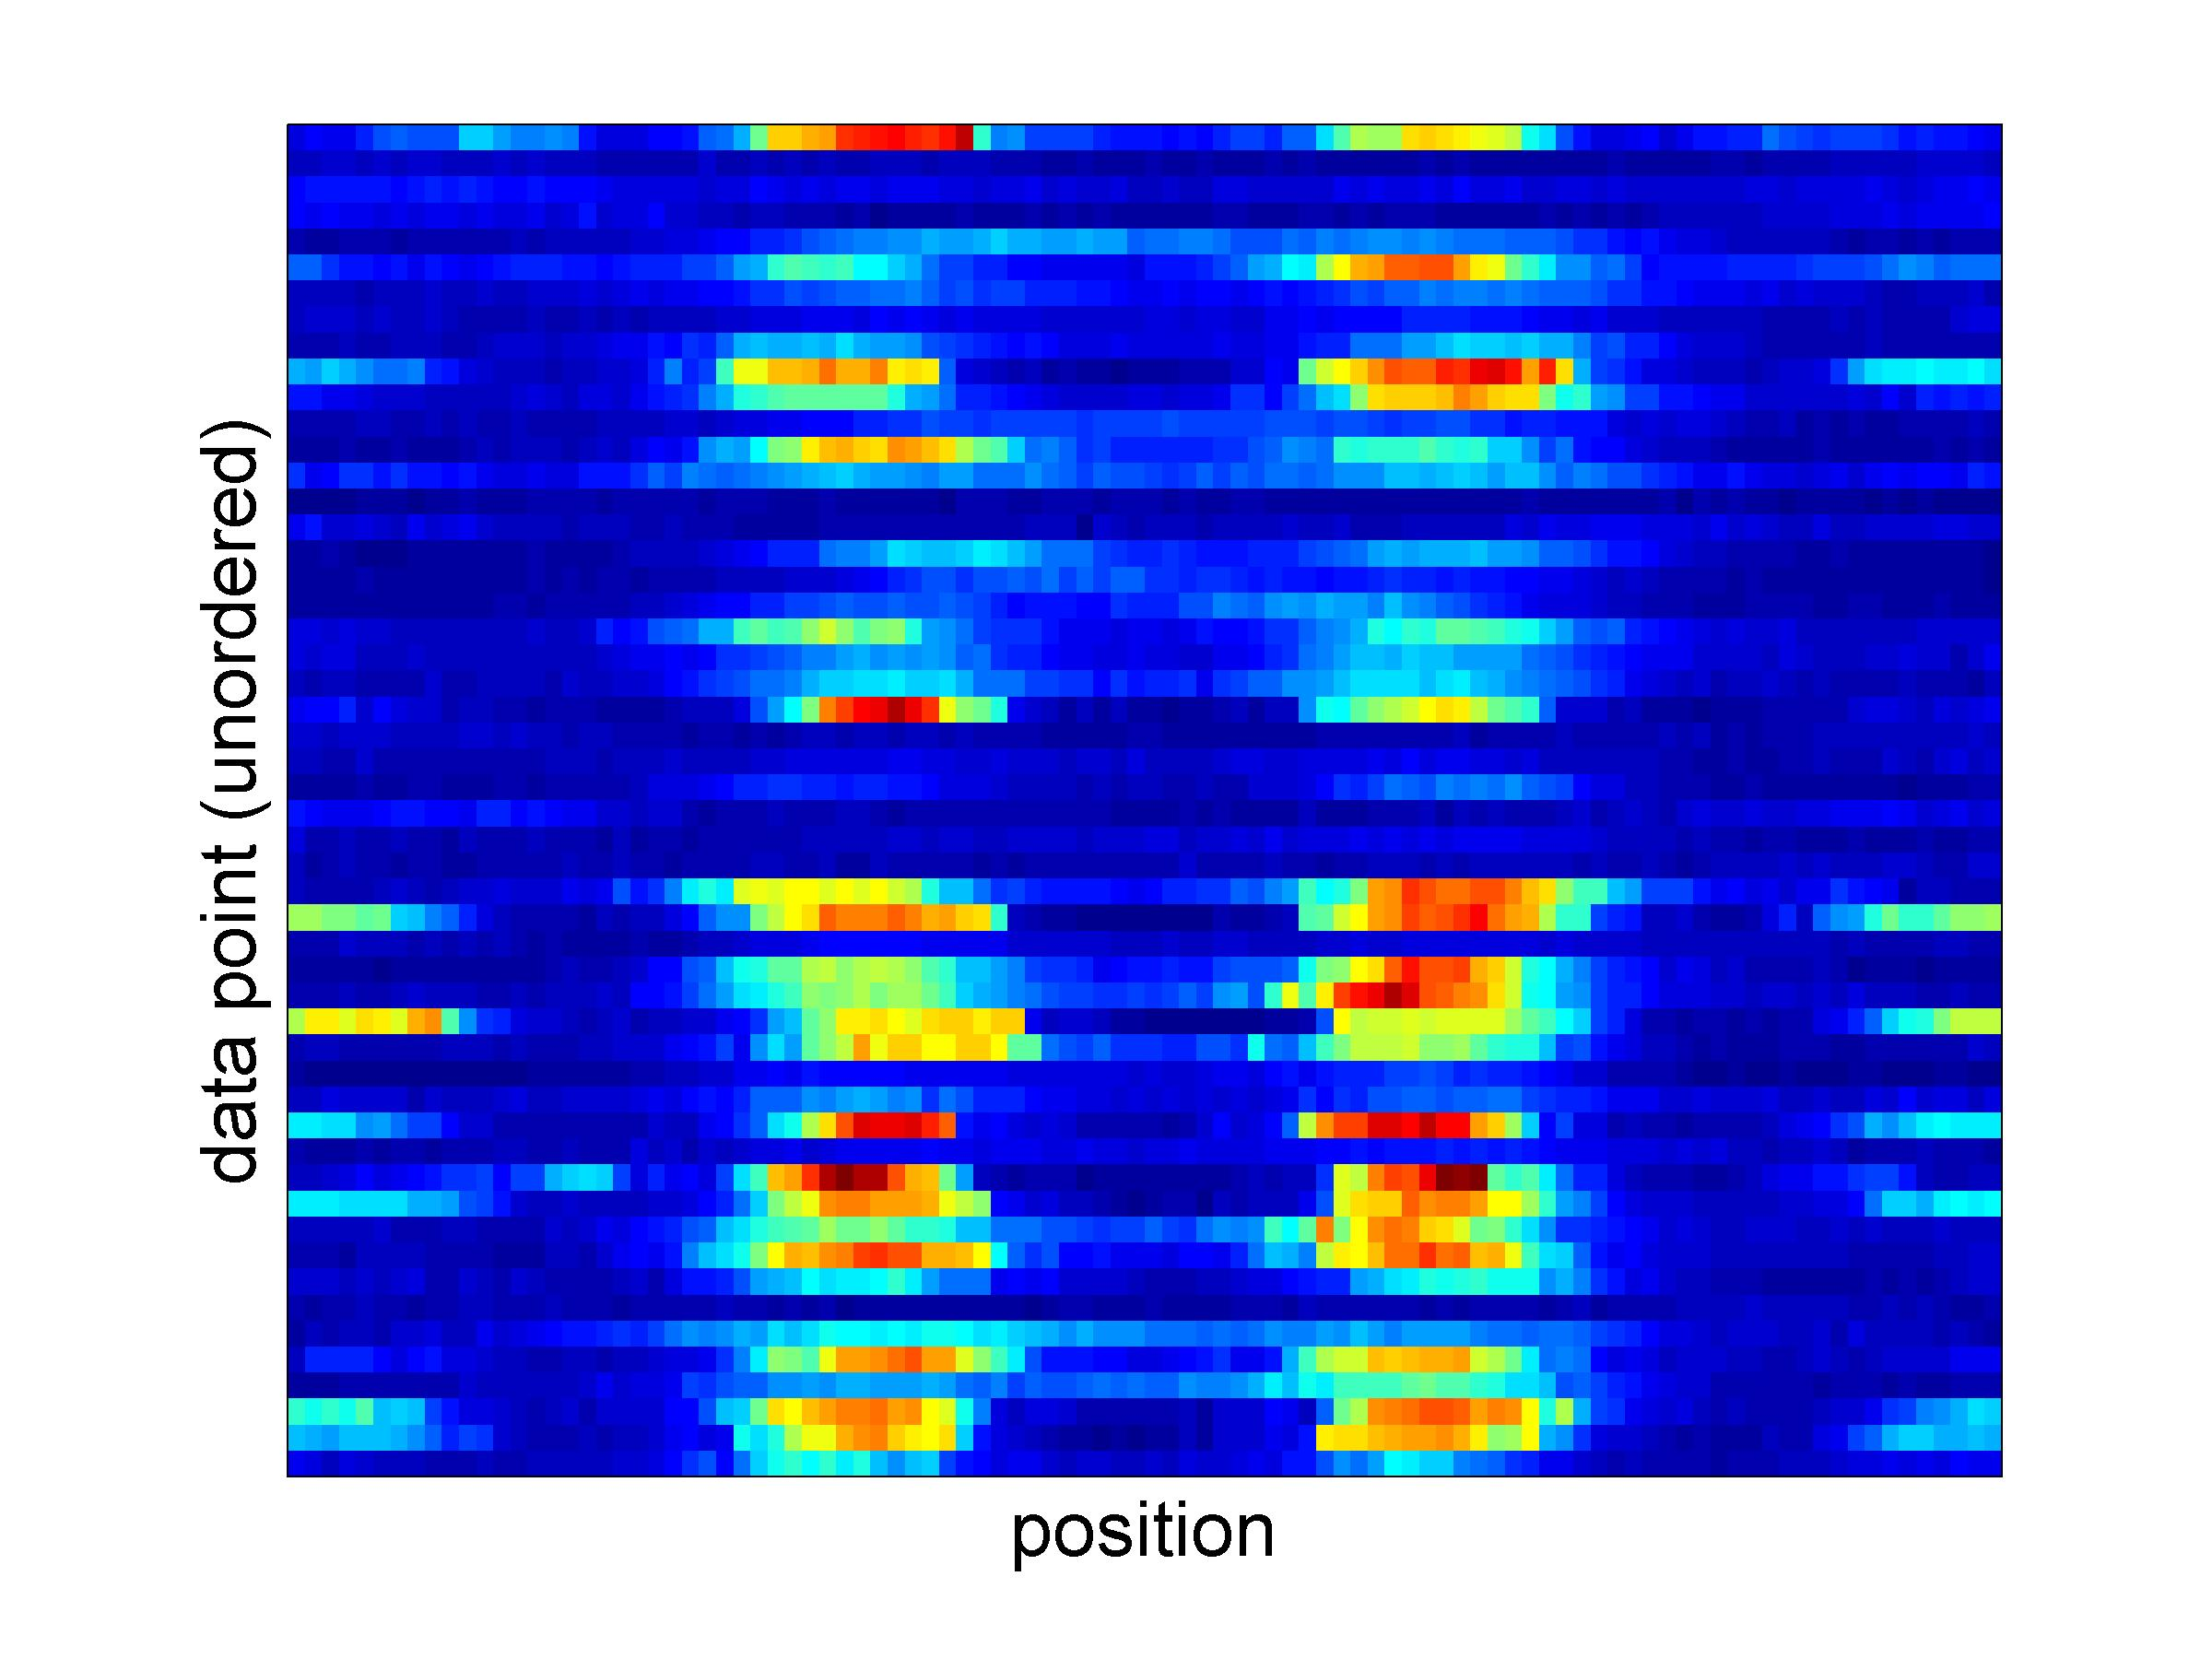
\includegraphics[width=\textwidth]{data_unordered}
\caption{}
\end{subfigure}
\begin{subfigure}{0.3\textwidth}
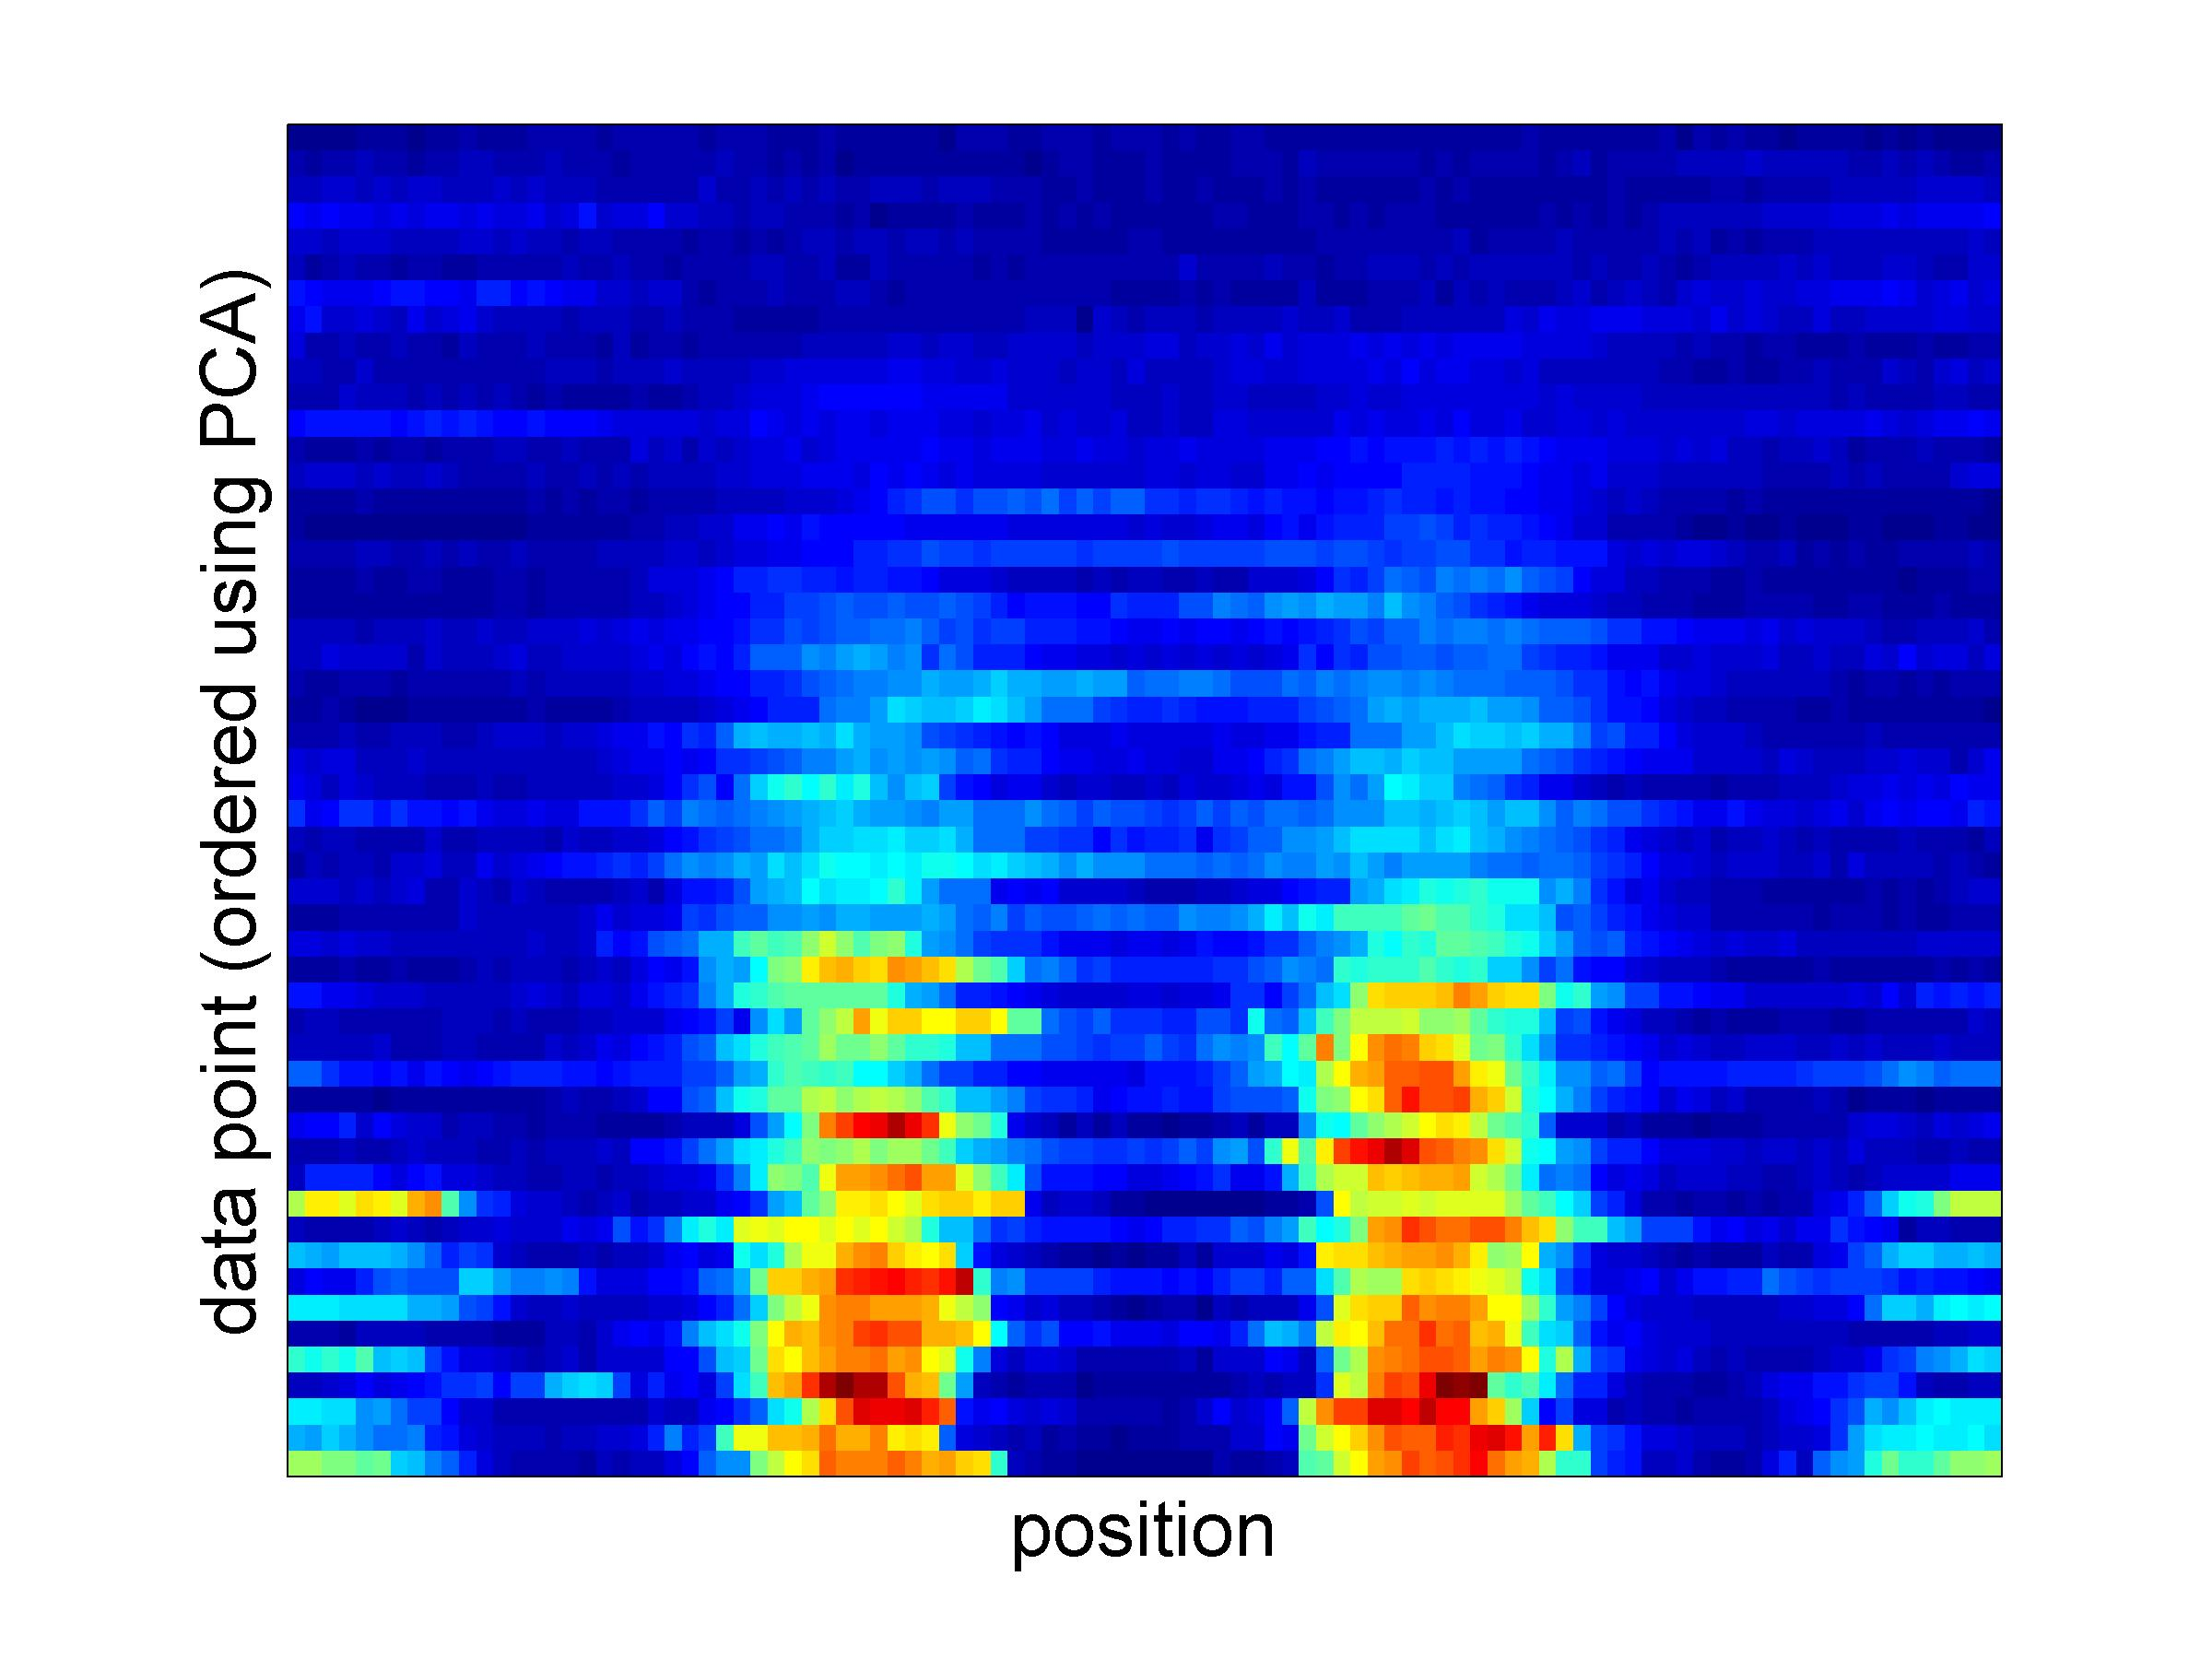
\includegraphics[width=\textwidth]{data_ordered_PCA}
\caption{}
\end{subfigure}
\begin{subfigure}{0.3\textwidth}
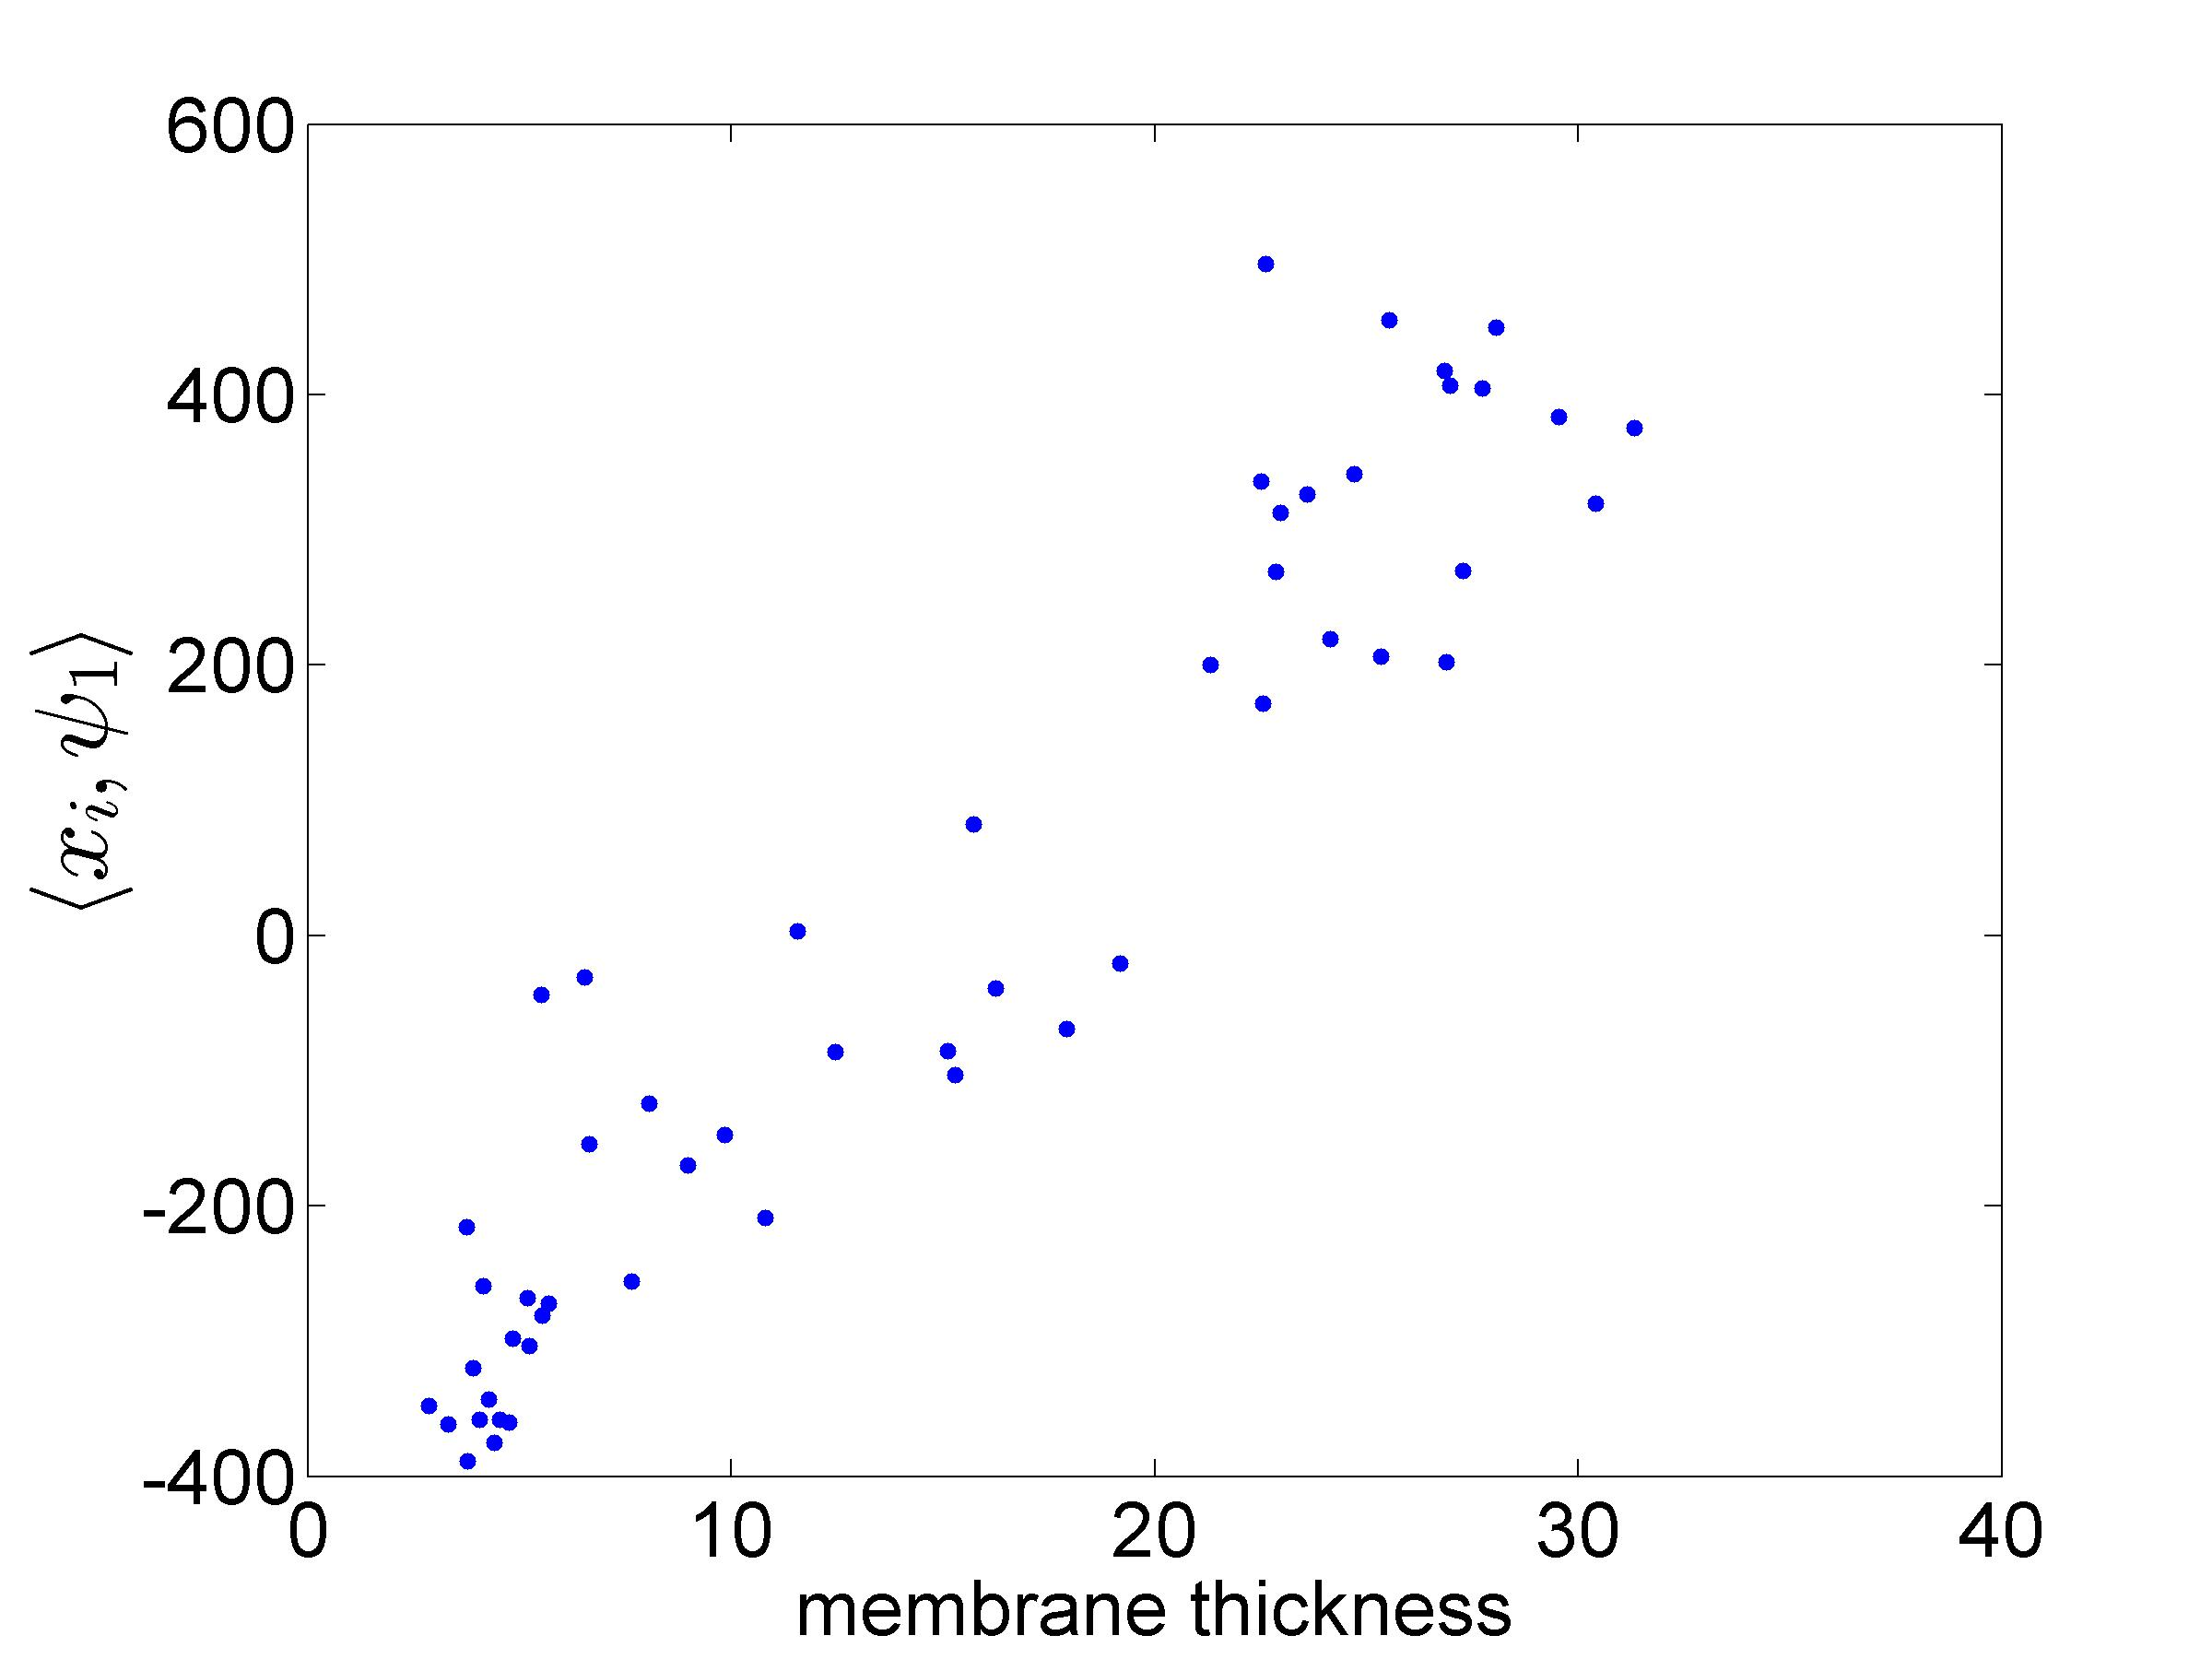
\includegraphics[width=\textwidth]{PCA_time_corr}
\caption{}
\end{subfigure}
\caption{{\bf Ordering dpERK concentration profiles using PCA.} (a) Concentration profiles of dpERK for many embryos. Each row represents a different embryo fixed at a slightly different developmental time.
(b) Concentration profiles of dpERK from (a), now ordered by the first PCA projection coefficient.
(c) Correlation between the first PCA projection coefficient and the membrane thickness.}
\label{fig:PCA_ordering}
\end{figure}

\subsection*{dpERK concentration profiles ordered using Diffusion Maps}
\begin{figure}[H]
\begin{subfigure}{0.3\textwidth}
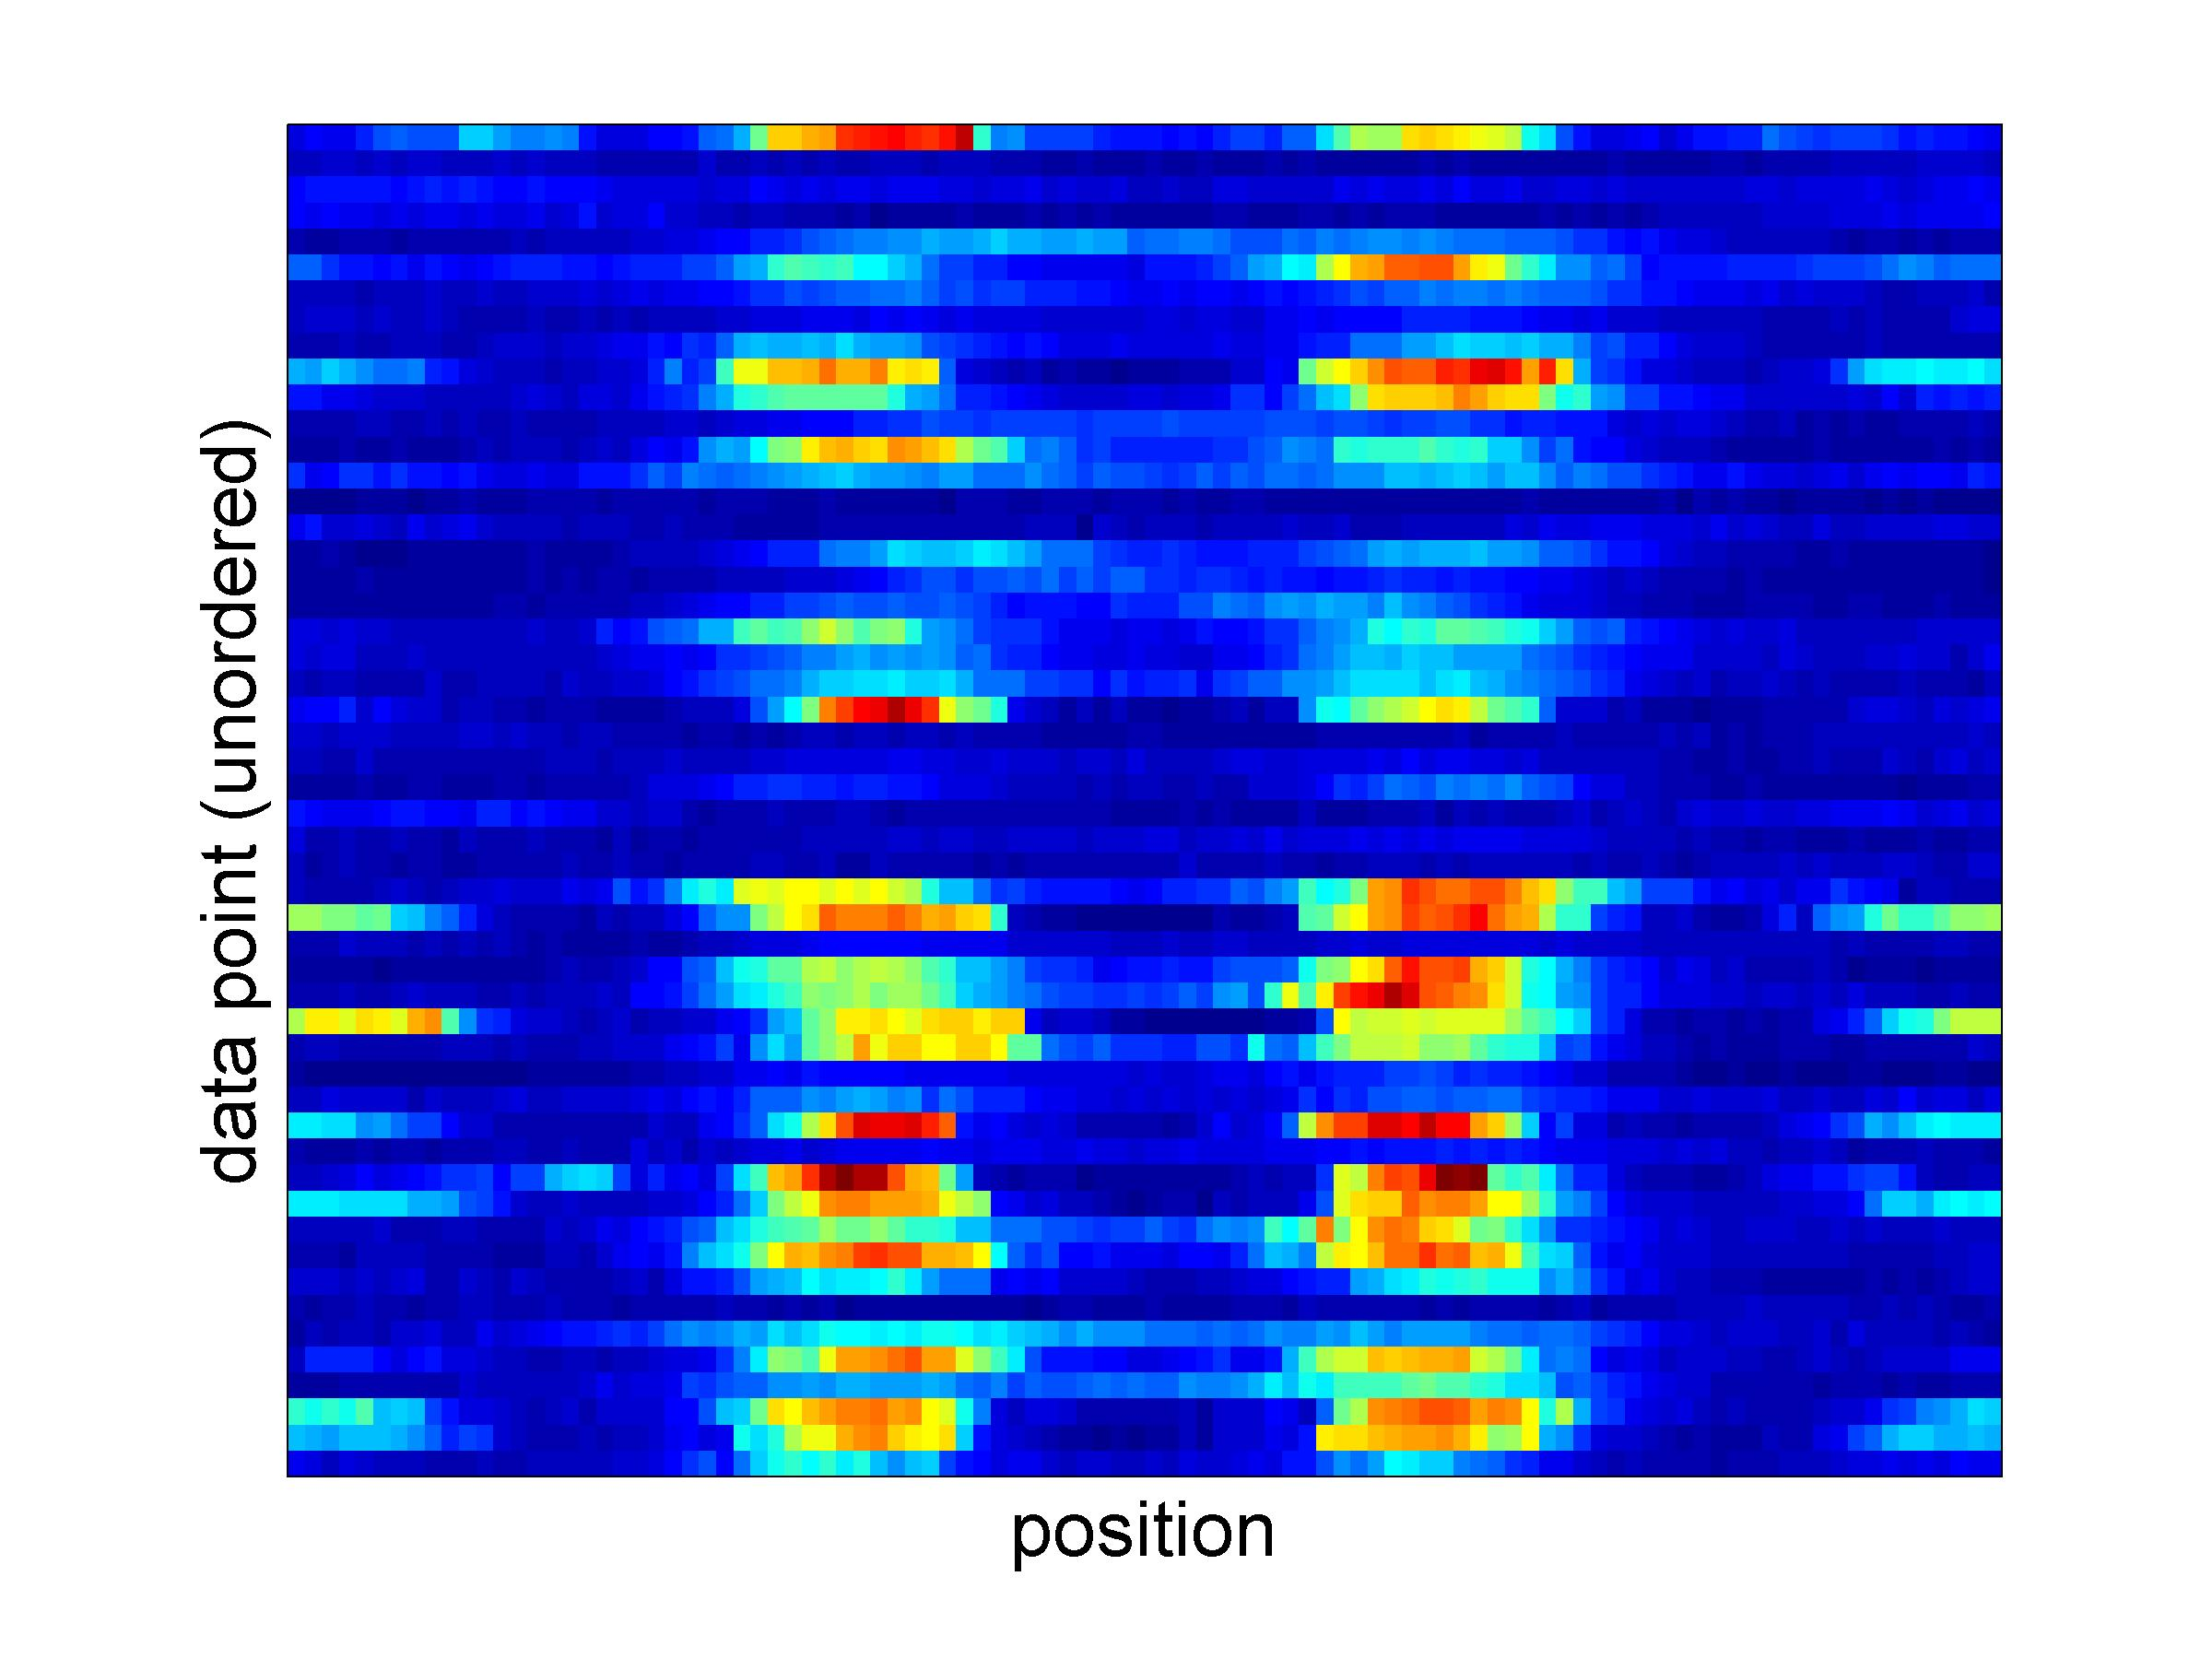
\includegraphics[width=\textwidth]{data_unordered}
\caption{}
\end{subfigure}
\begin{subfigure}{0.3\textwidth}
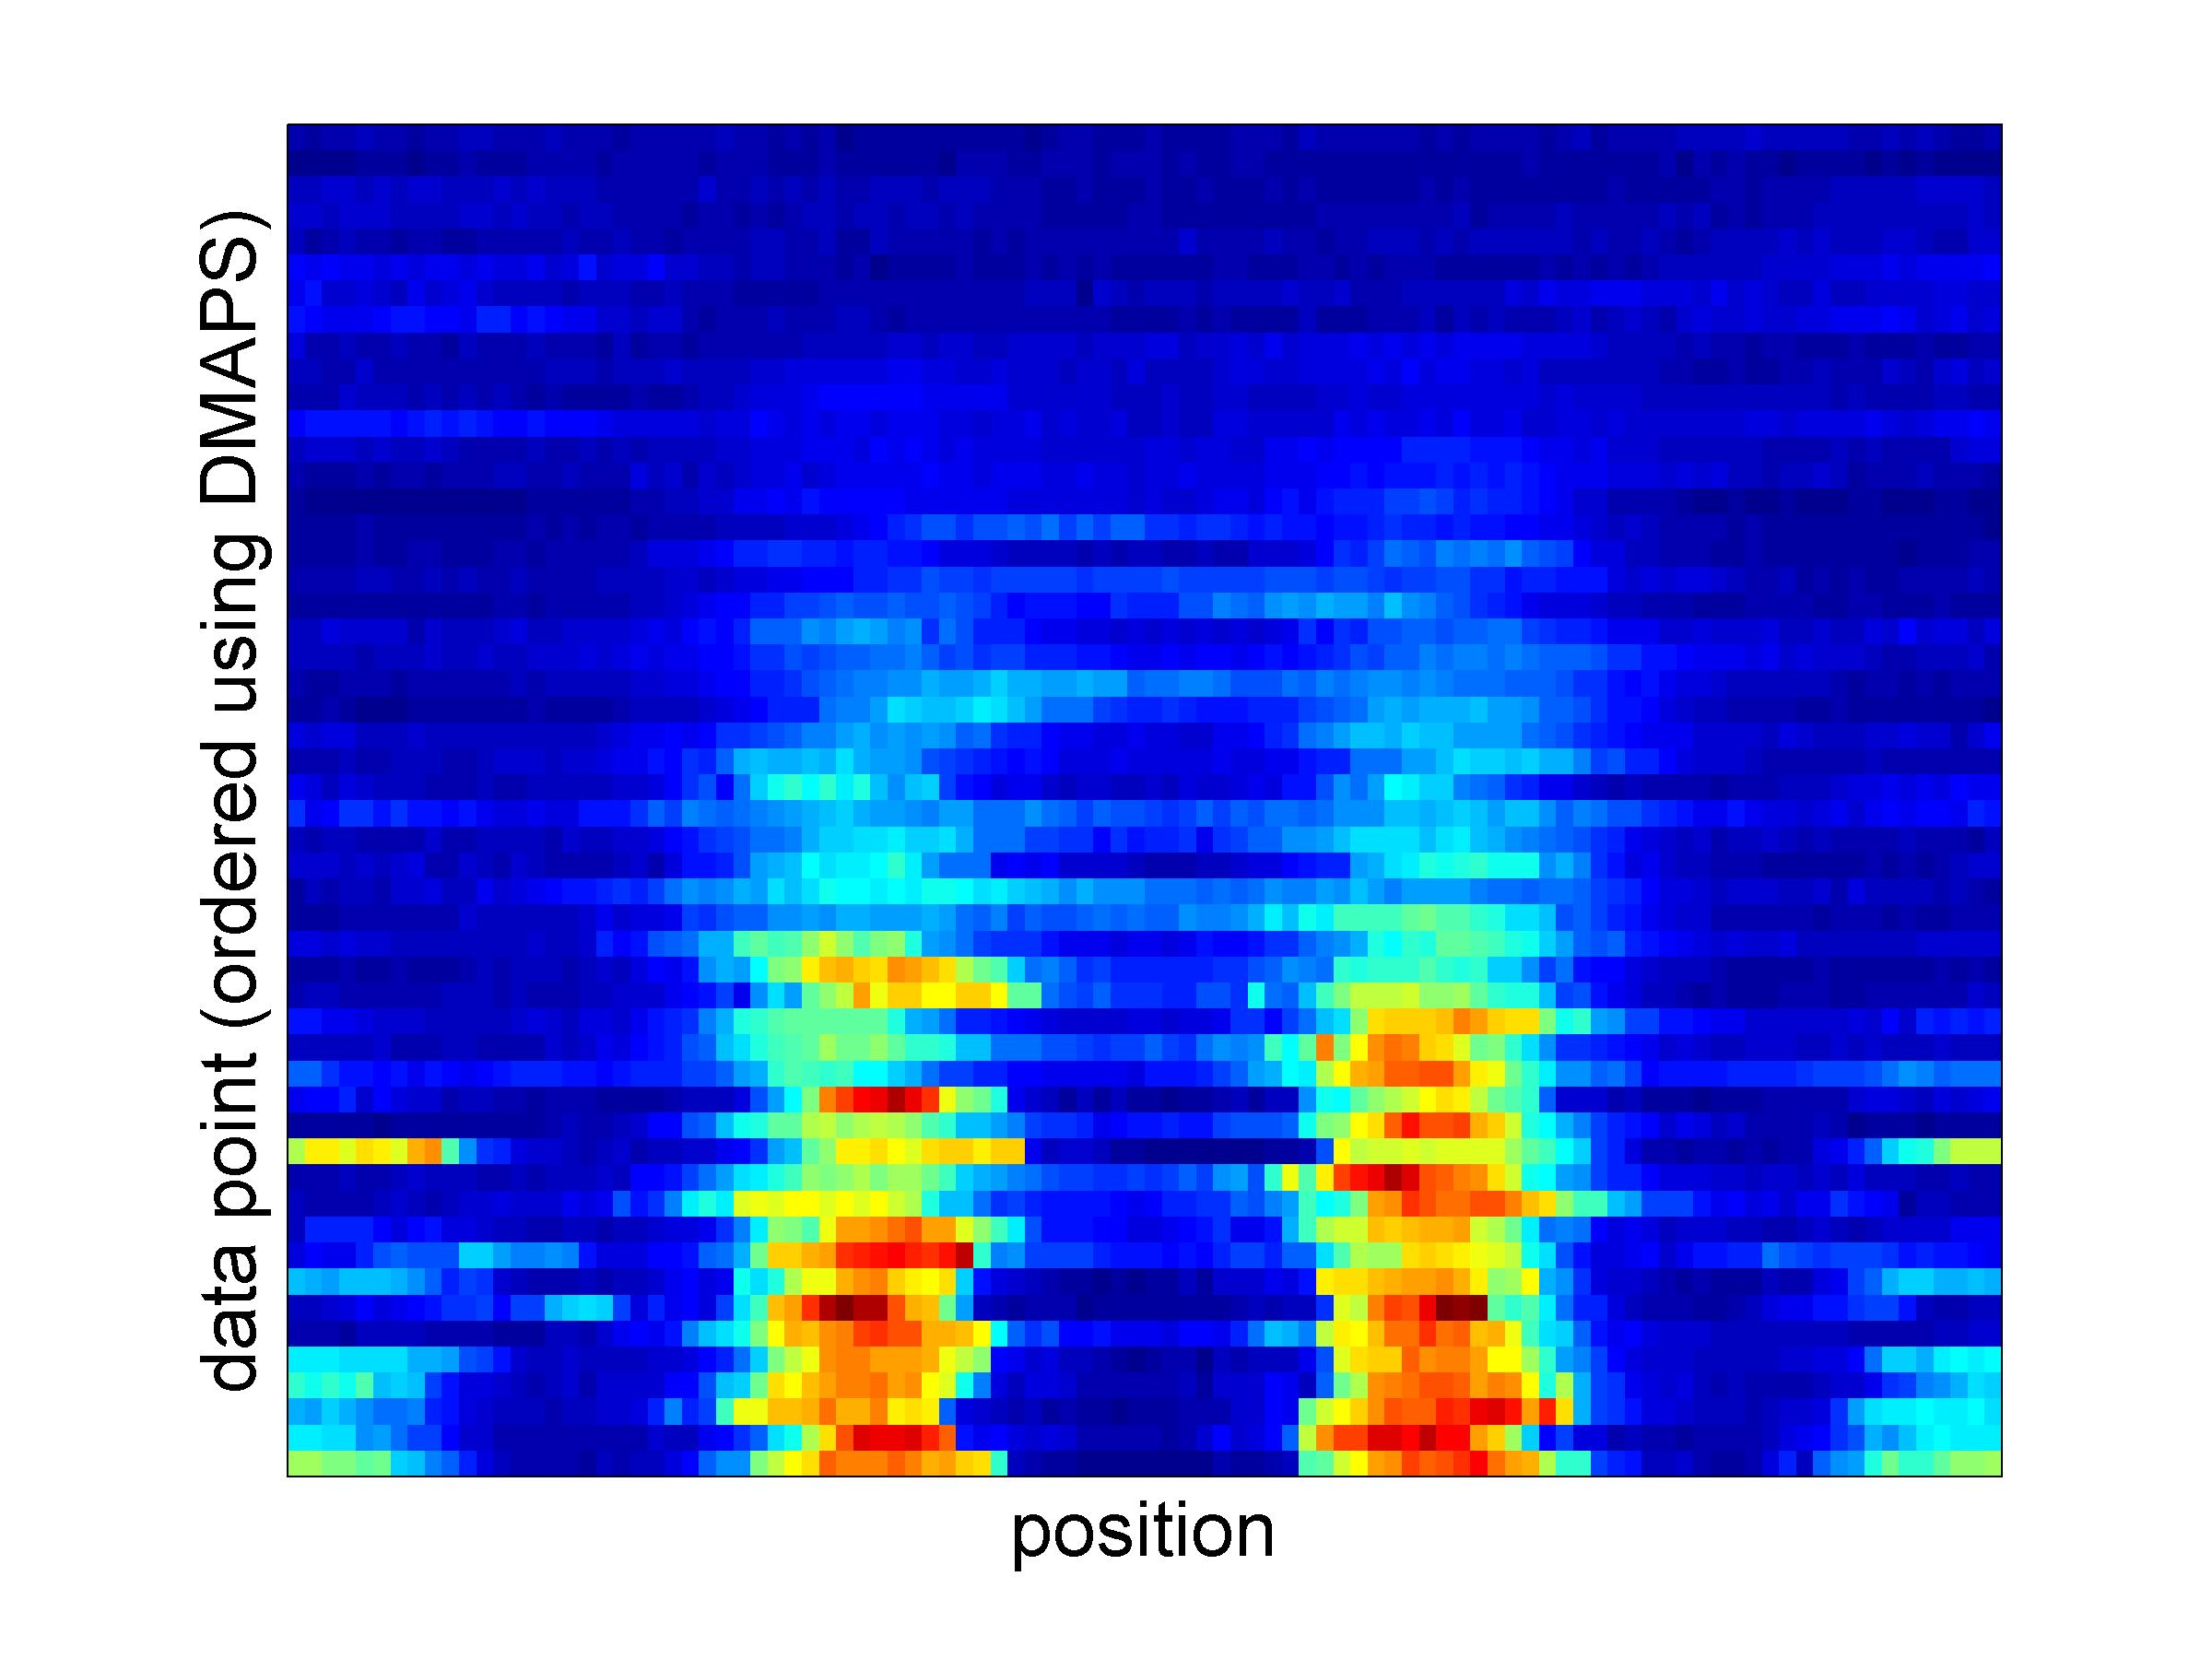
\includegraphics[width=\textwidth]{data_ordered_DMAPS}
\caption{}
\end{subfigure}
\begin{subfigure}{0.3\textwidth}
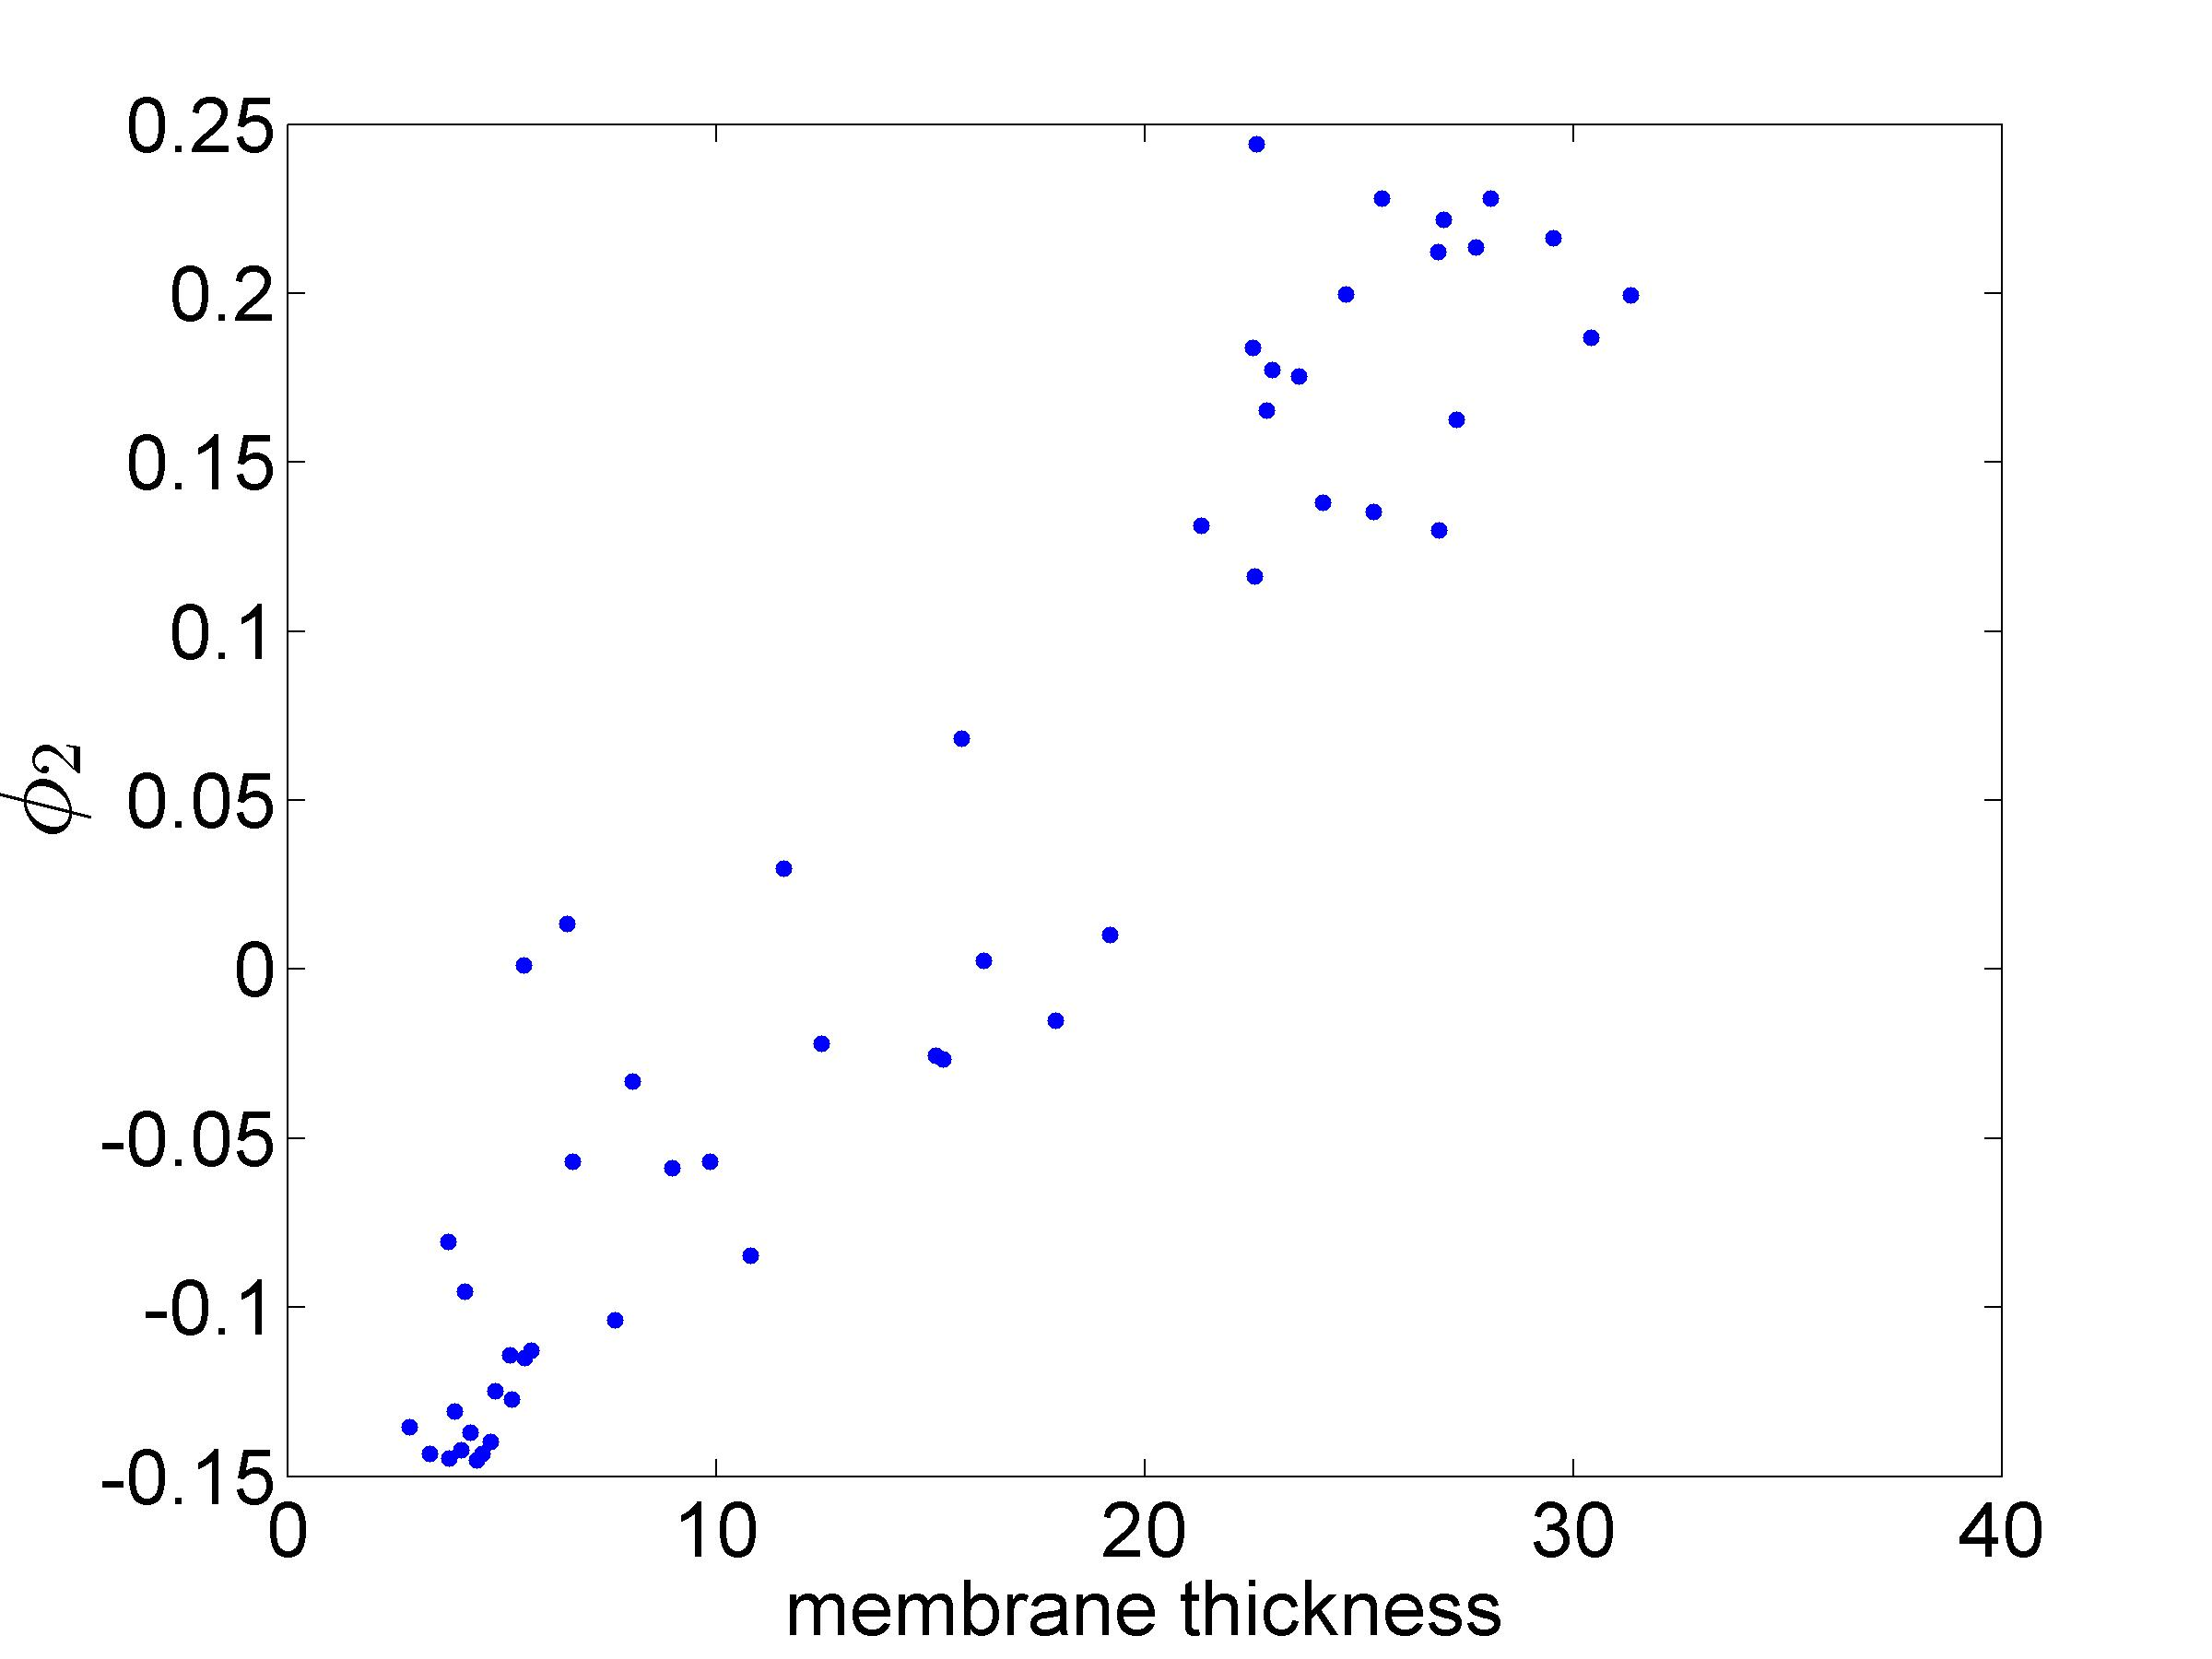
\includegraphics[width=\textwidth]{DMAPS_time_corr}
\caption{}
\end{subfigure}
\caption{{\bf Ordering dpERK concentration profiles using DMAPS.} (a) Concentration profiles of dpERK for many embryos. Each row represents a different embryo fixed at a slightly different developmental time.
(b) Concentration profiles of dpERK from (a), now ordered by the first non-trivial DMAPS embedding coordinate.
(c) Correlation between the first (non-trivial) DMAPS embedding coordinate and the membrane thickness.}
\label{fig:DMAPS_ordering}
\end{figure}

\subsection*{dpERK concentration profiles aligned using angular synchronization}

\begin{figure}[H]
\begin{subfigure}{0.3\textwidth}
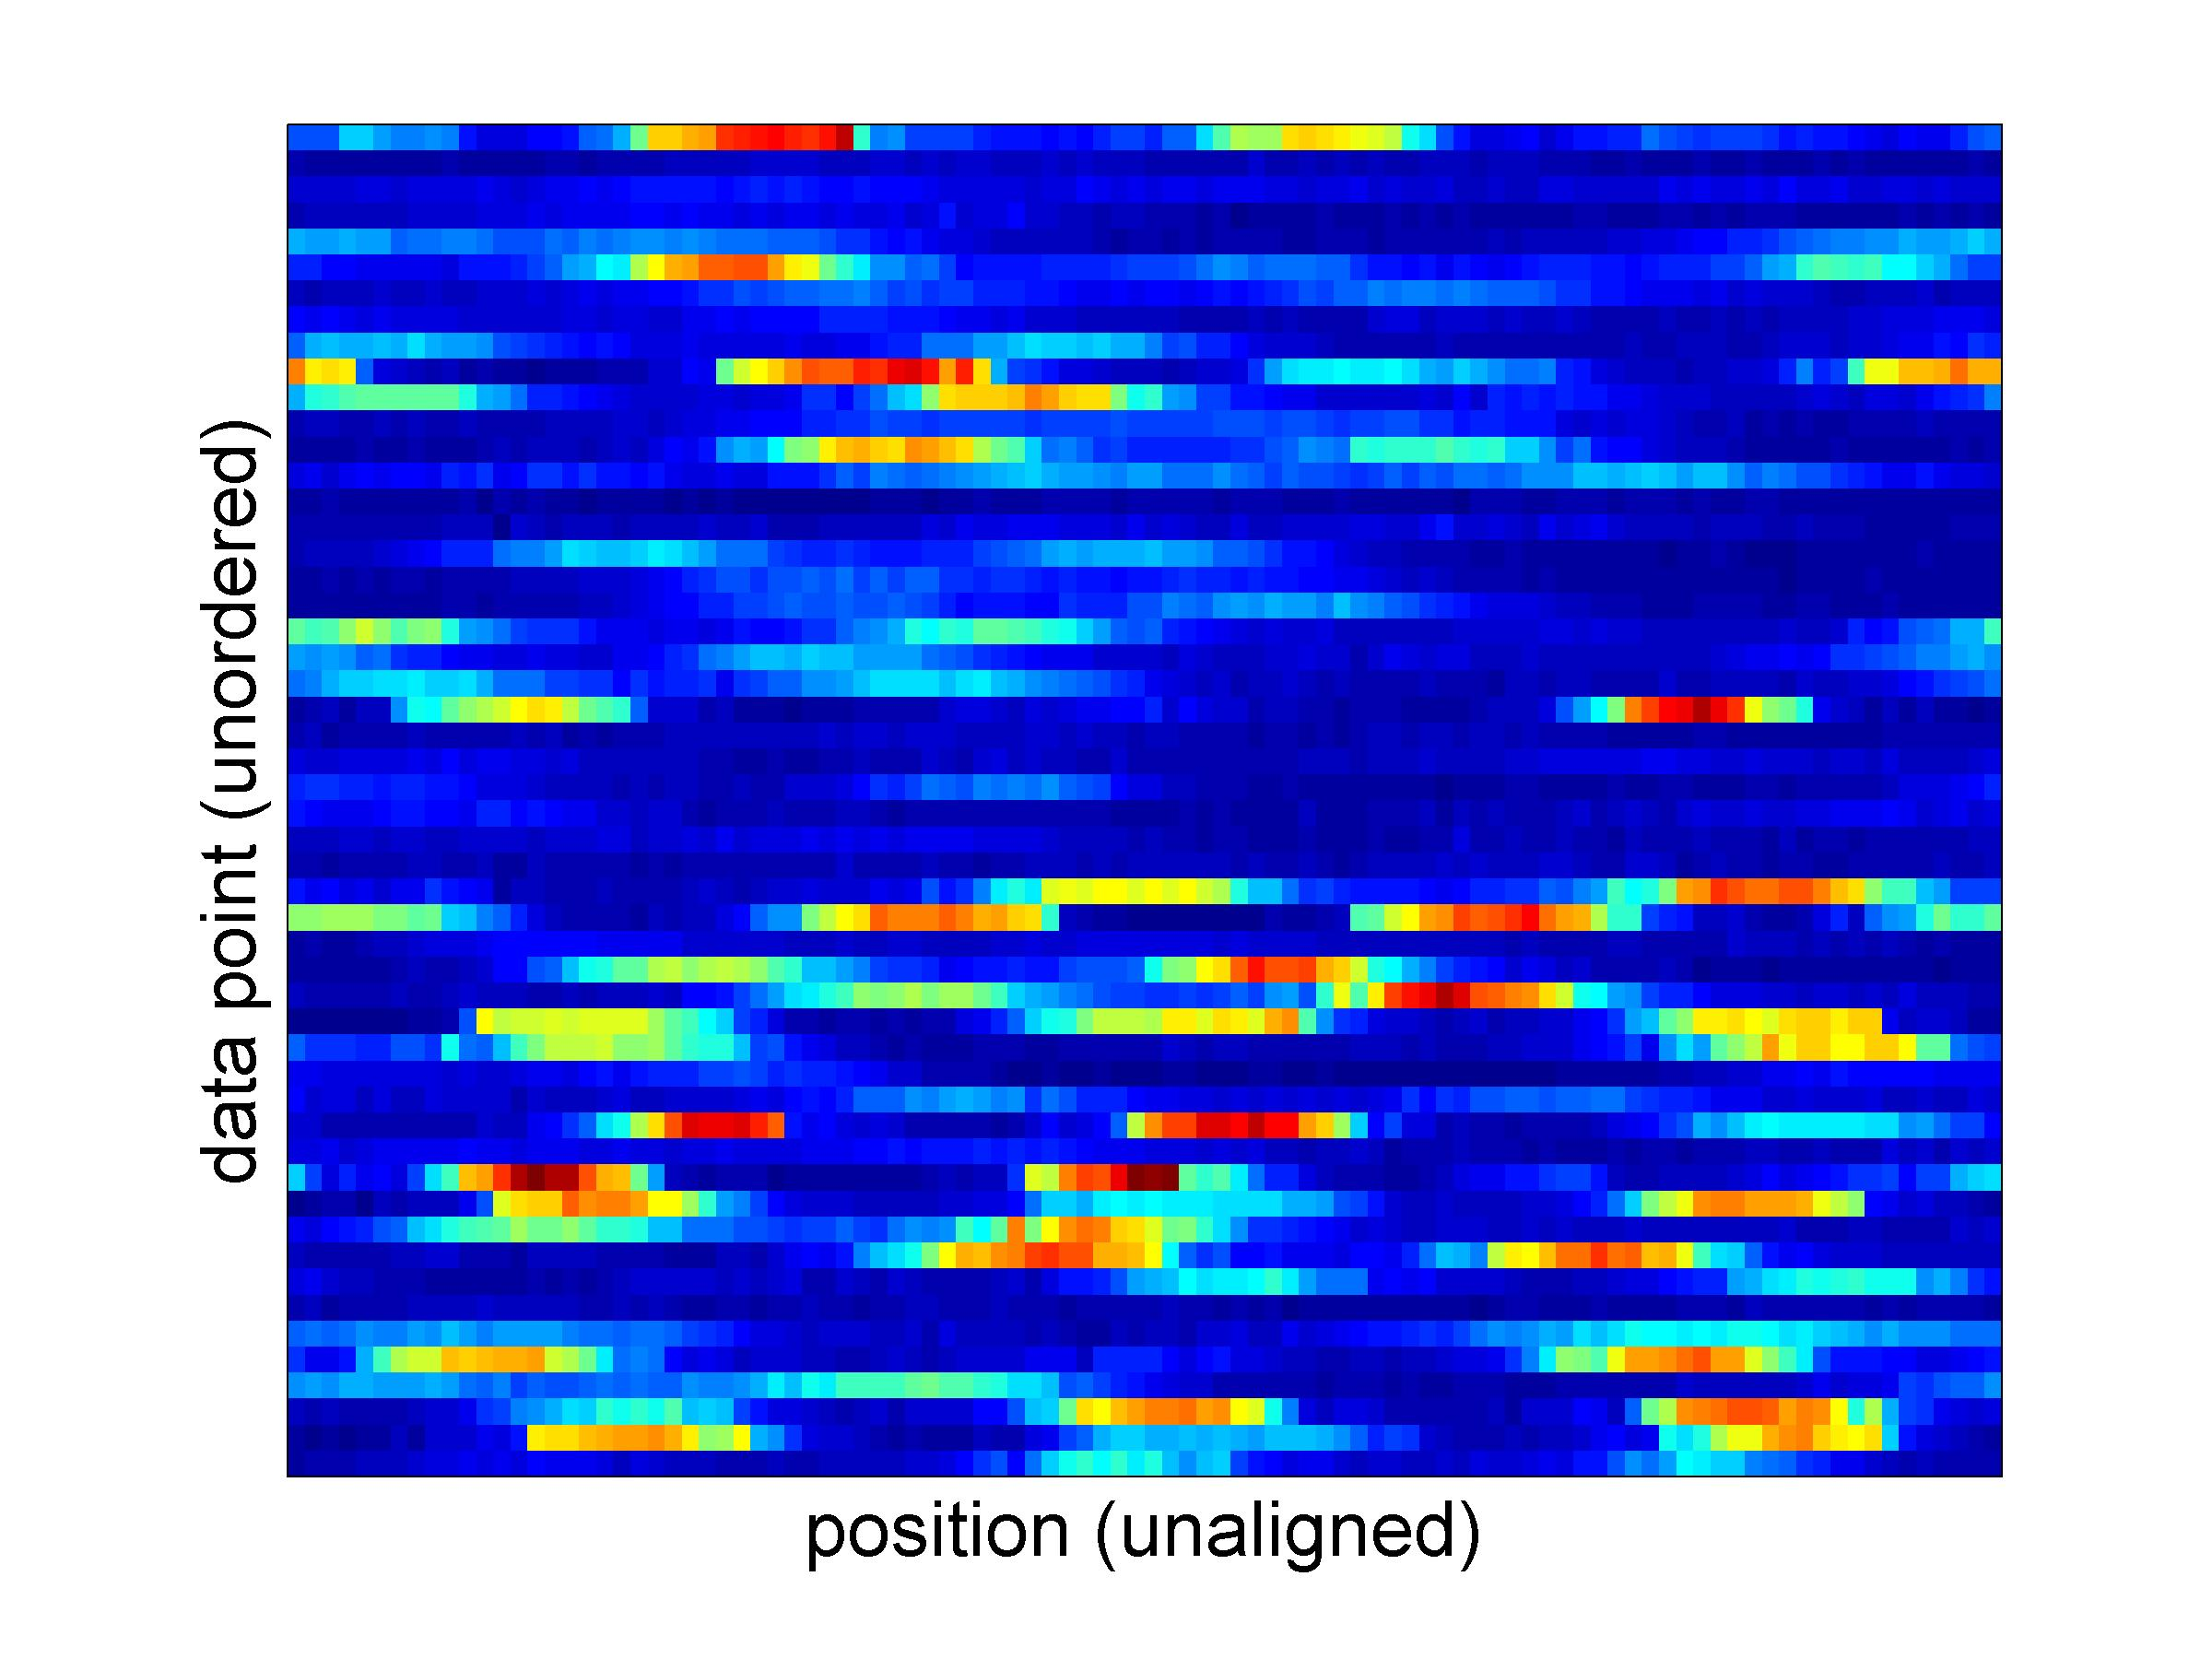
\includegraphics[width=\textwidth]{data_unaligned_unordered}
\caption{}
\end{subfigure}
\begin{subfigure}{0.3\textwidth}
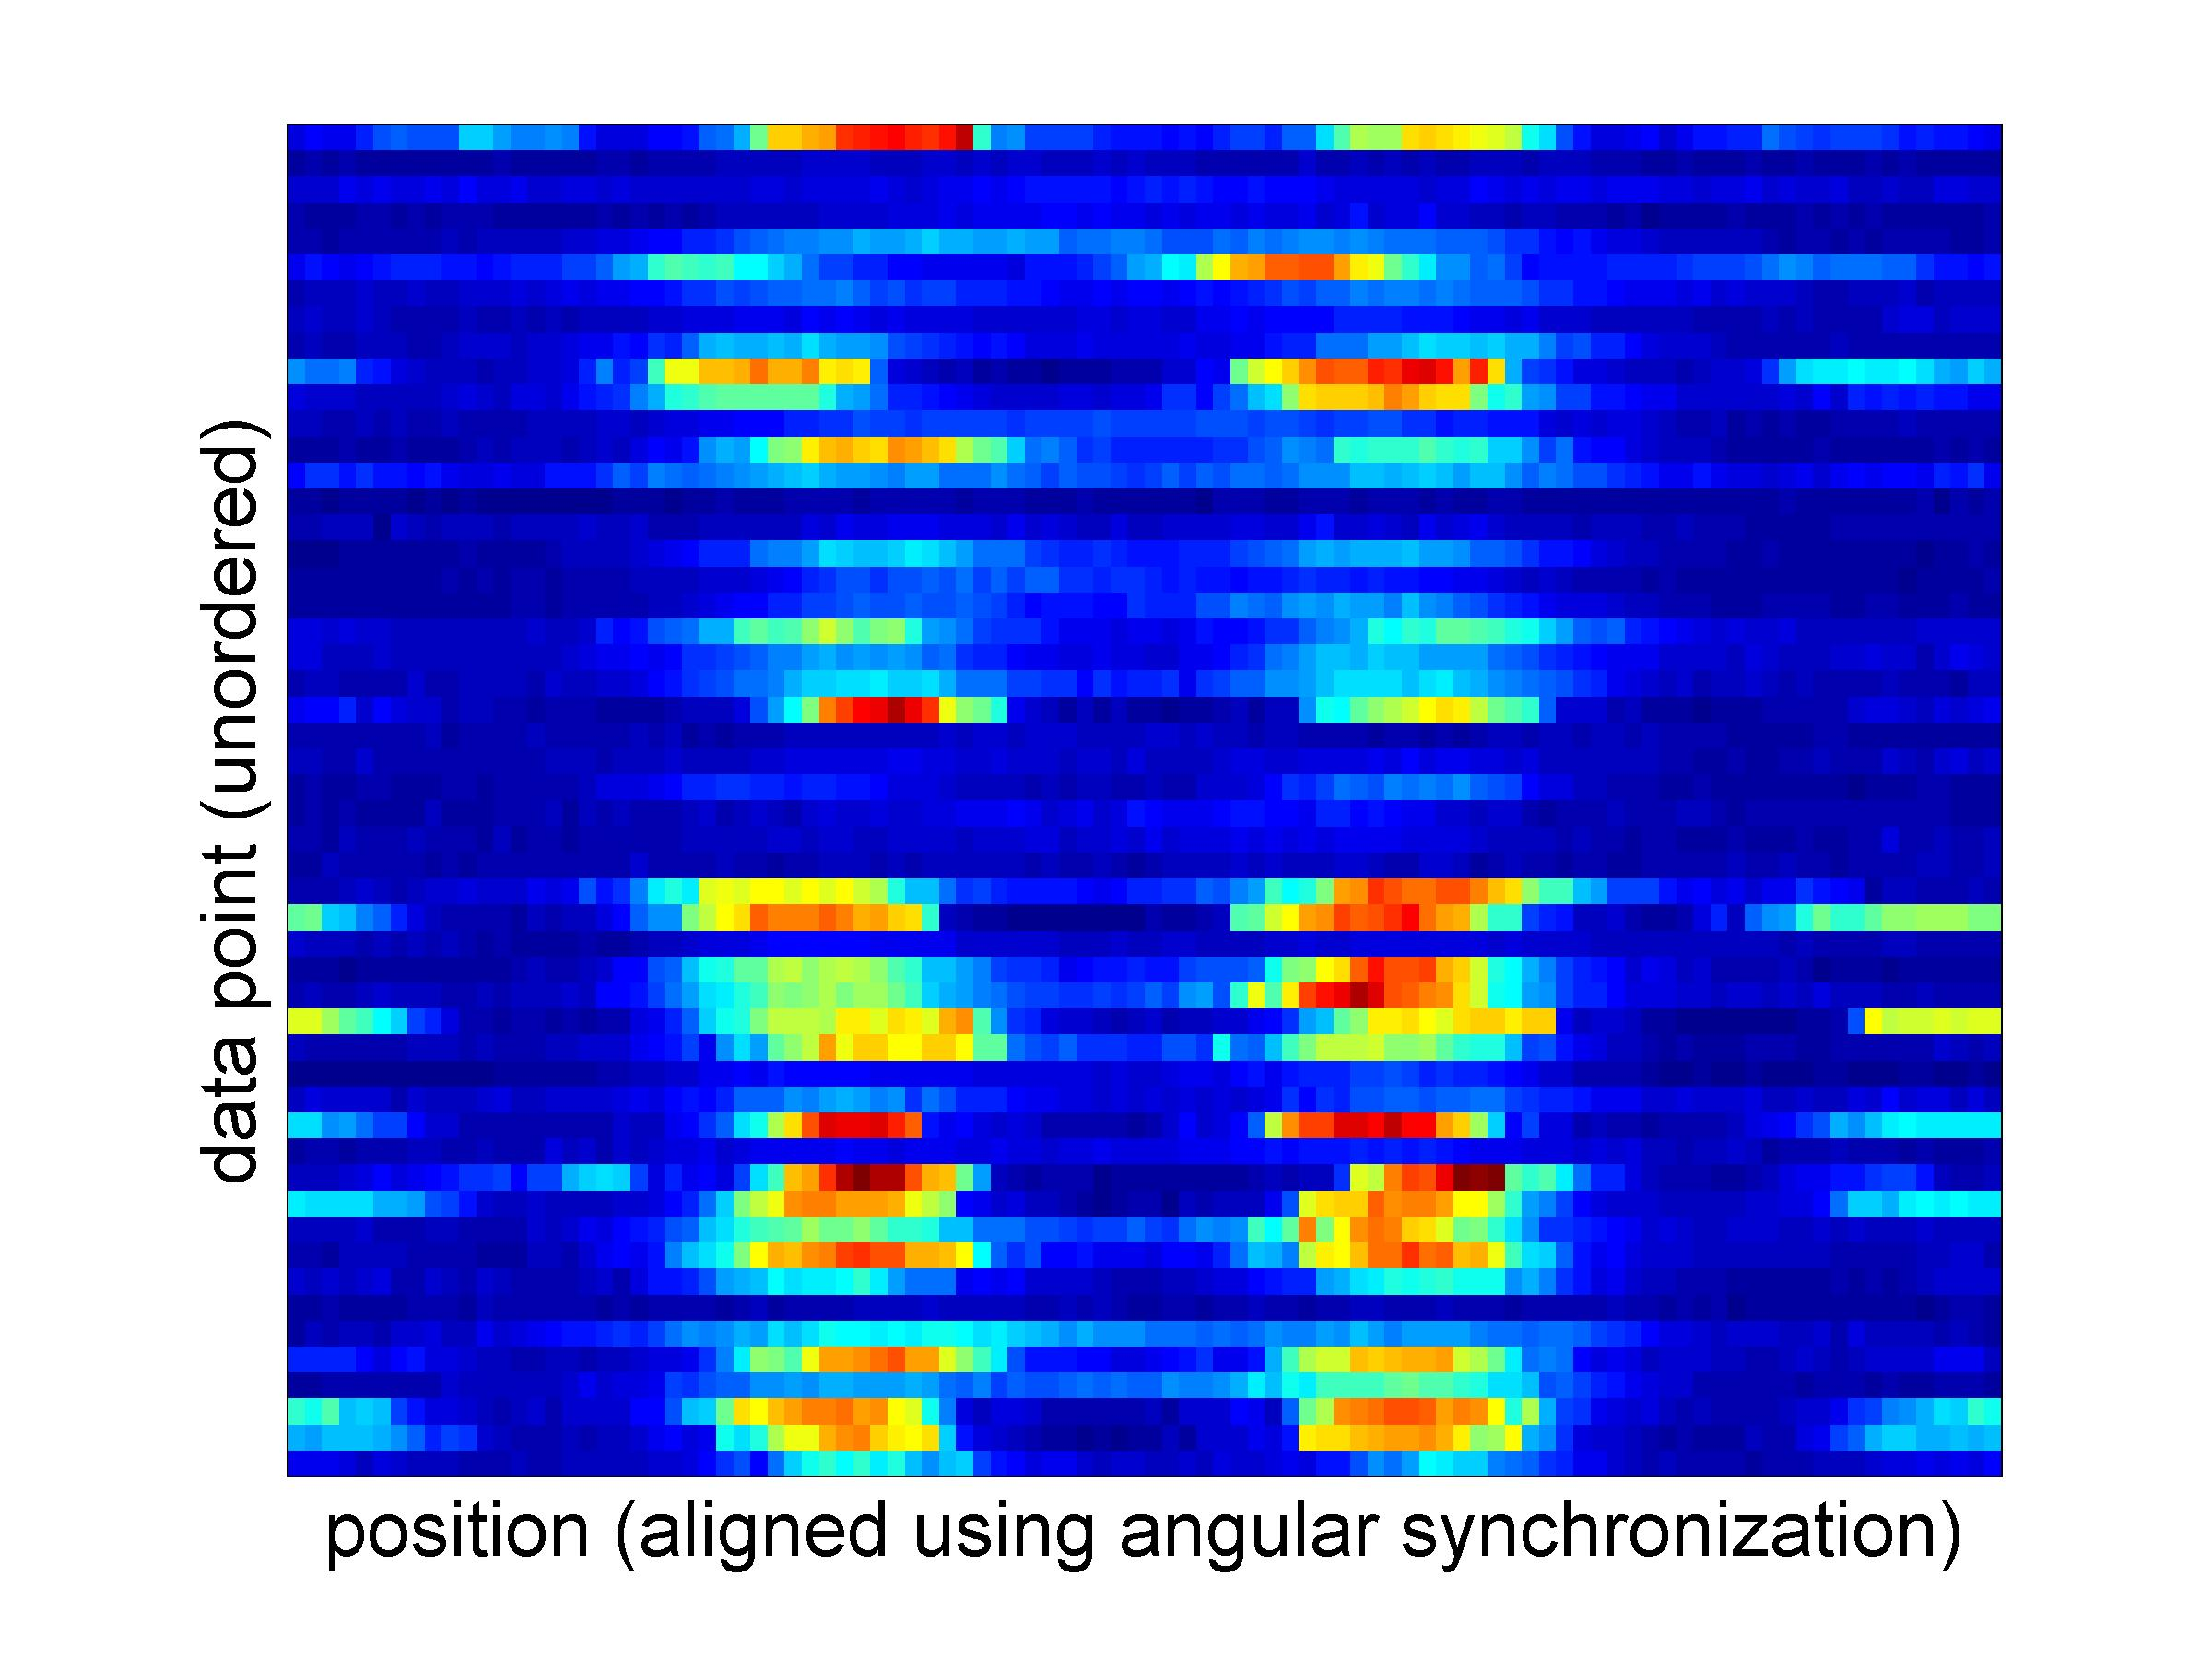
\includegraphics[width=\textwidth]{data_aligned_unordered}
\caption{}
\end{subfigure}
\begin{subfigure}{0.3\textwidth}
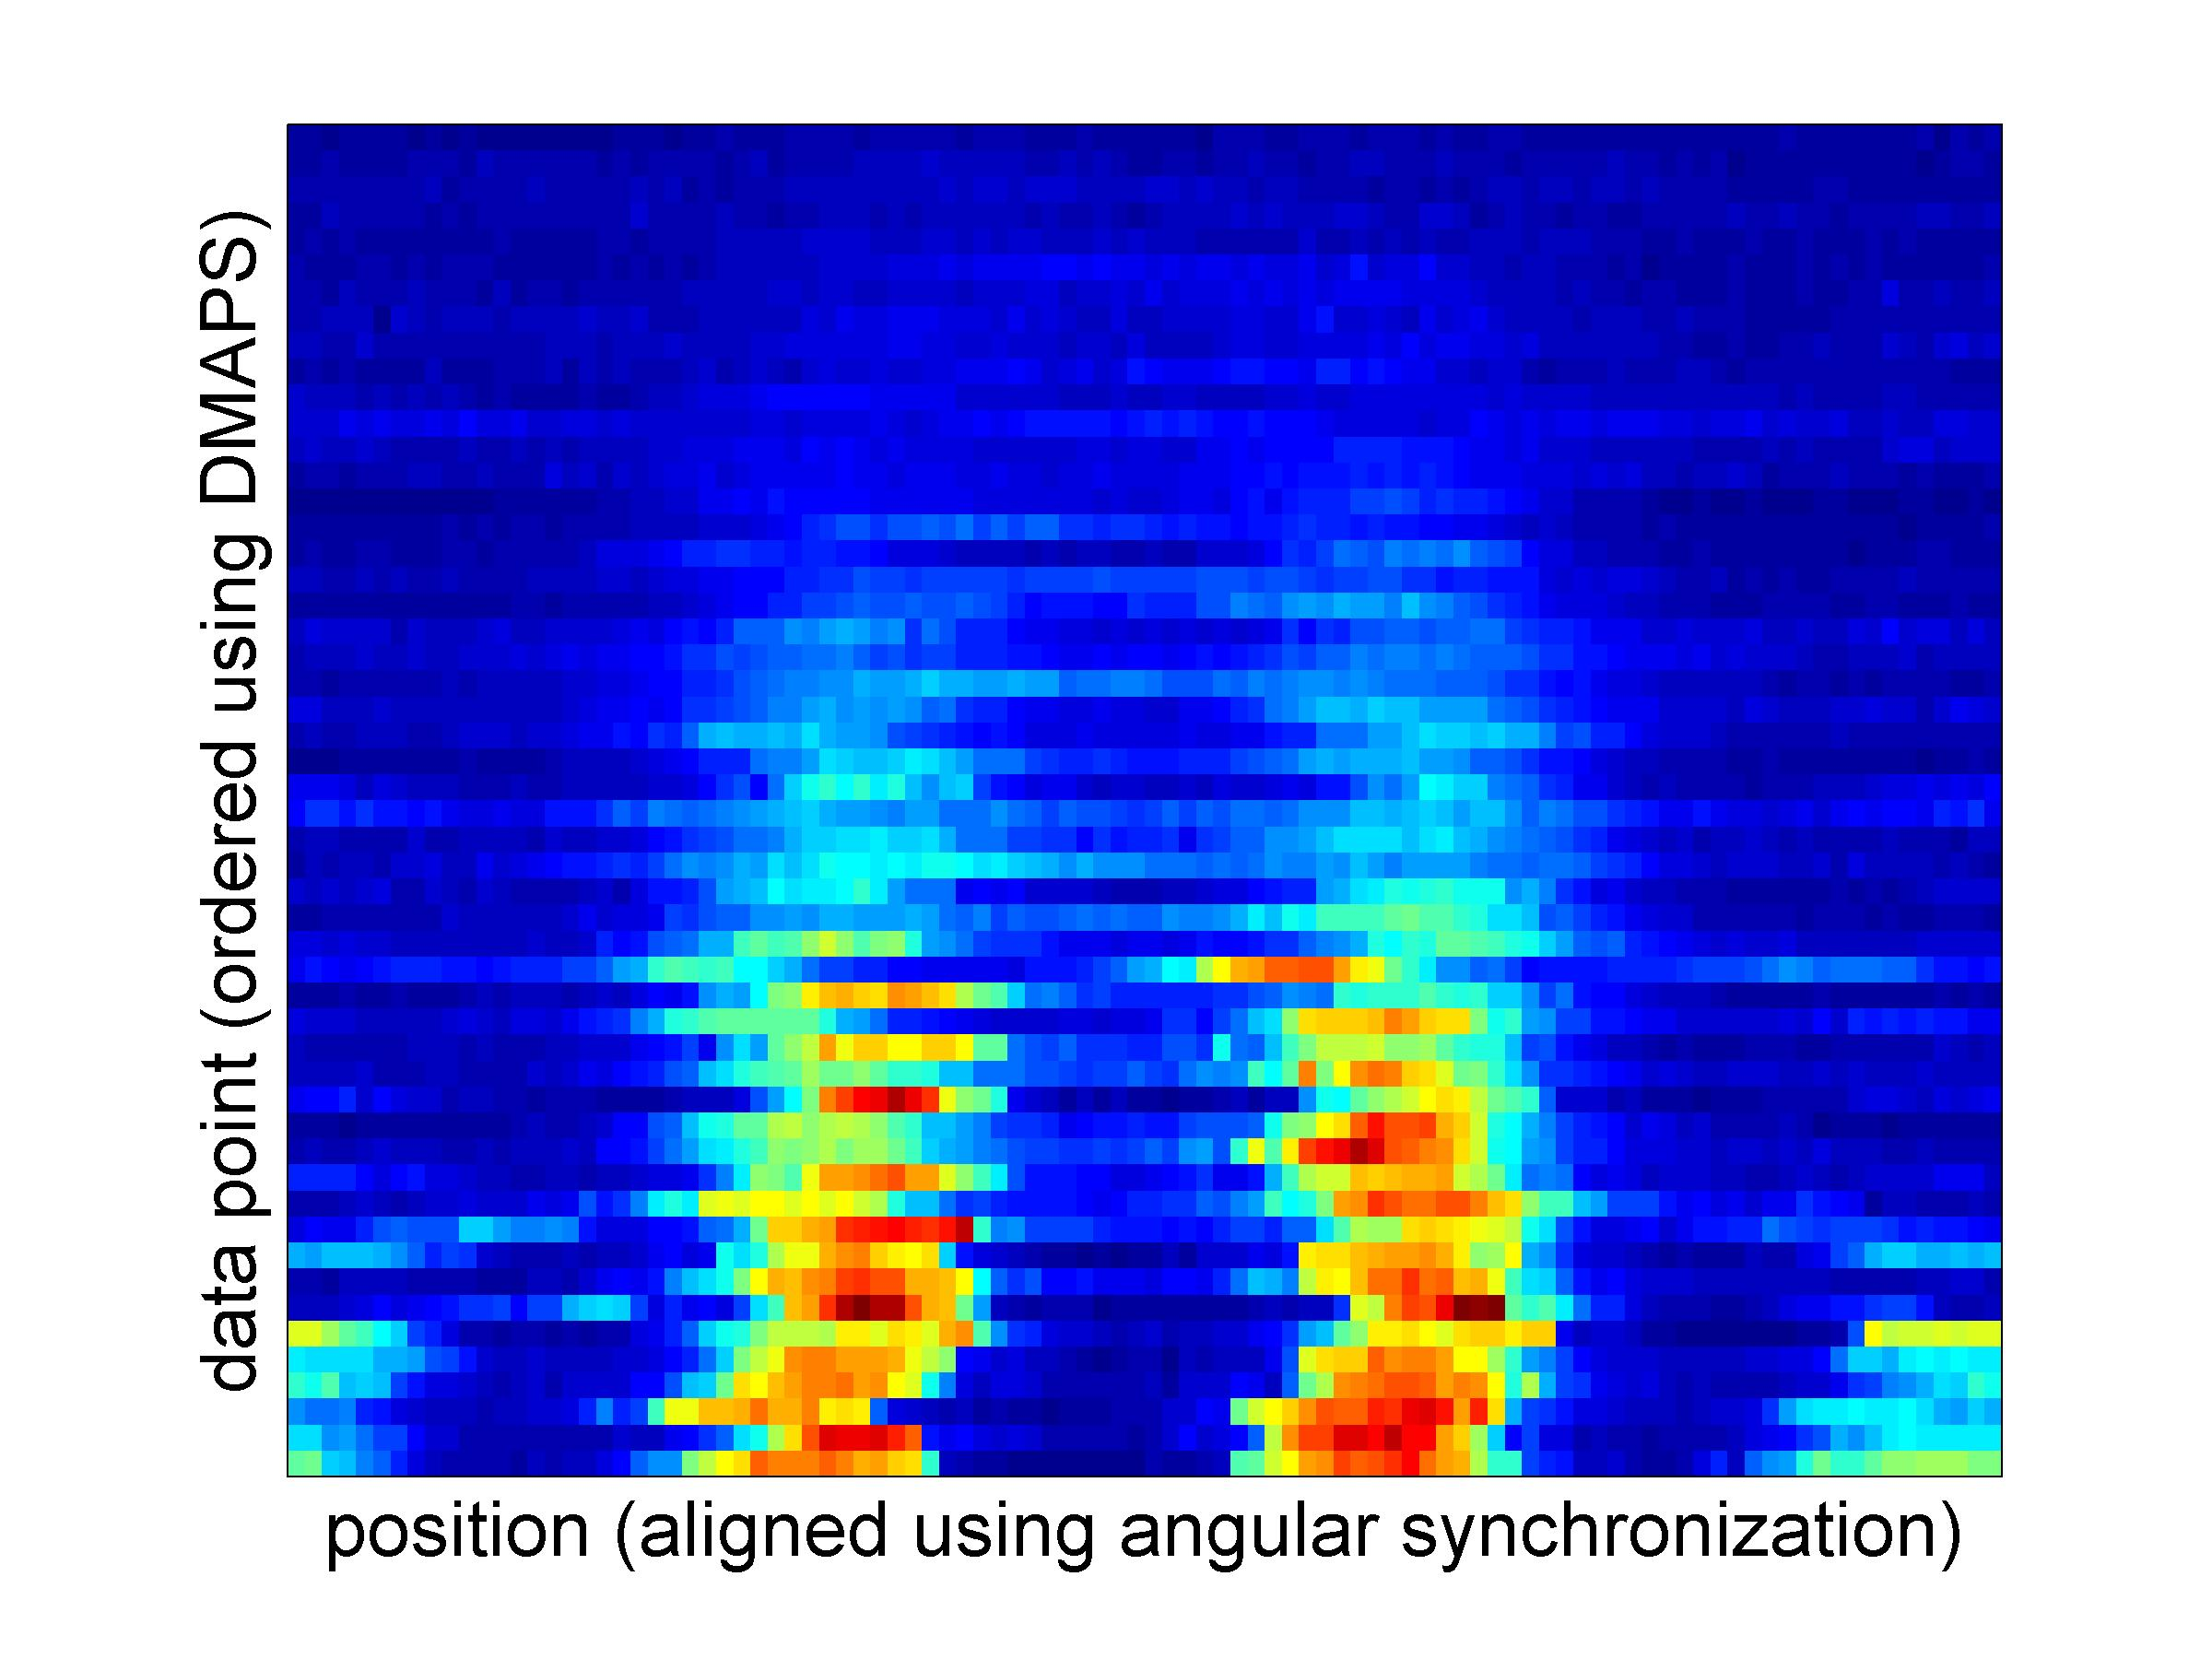
\includegraphics[width=\textwidth]{data_ordered_angsynch}
\caption{}
\end{subfigure}
\caption{{\bf Ordering spatially unaligned dpERK concentration profiles.} (a) Concentration profiles of dpERK for many embryos. Each row represents a different embryo fixed at a slightly different developmental time. The circluar profiles have not been ``opened'' at the same point; rather, each profile was opened at a random point around the embryo. We are allowed to shift the (linear) profiles left and right.
(b) Concentration profiles of dpERK aligned using angular synchronization.
(c) Concentration profiles of dpERK aligned using angular synchronization and ordered by the first (non-trivial) DMAPS embedding coordinate.}
\label{fig:angsynch_ordering}
\end{figure}

\subsection*{dpERK concentration profiles aligned and ordered using vector diffusion maps}

\begin{figure}[H]
\begin{subfigure}{0.3\textwidth}
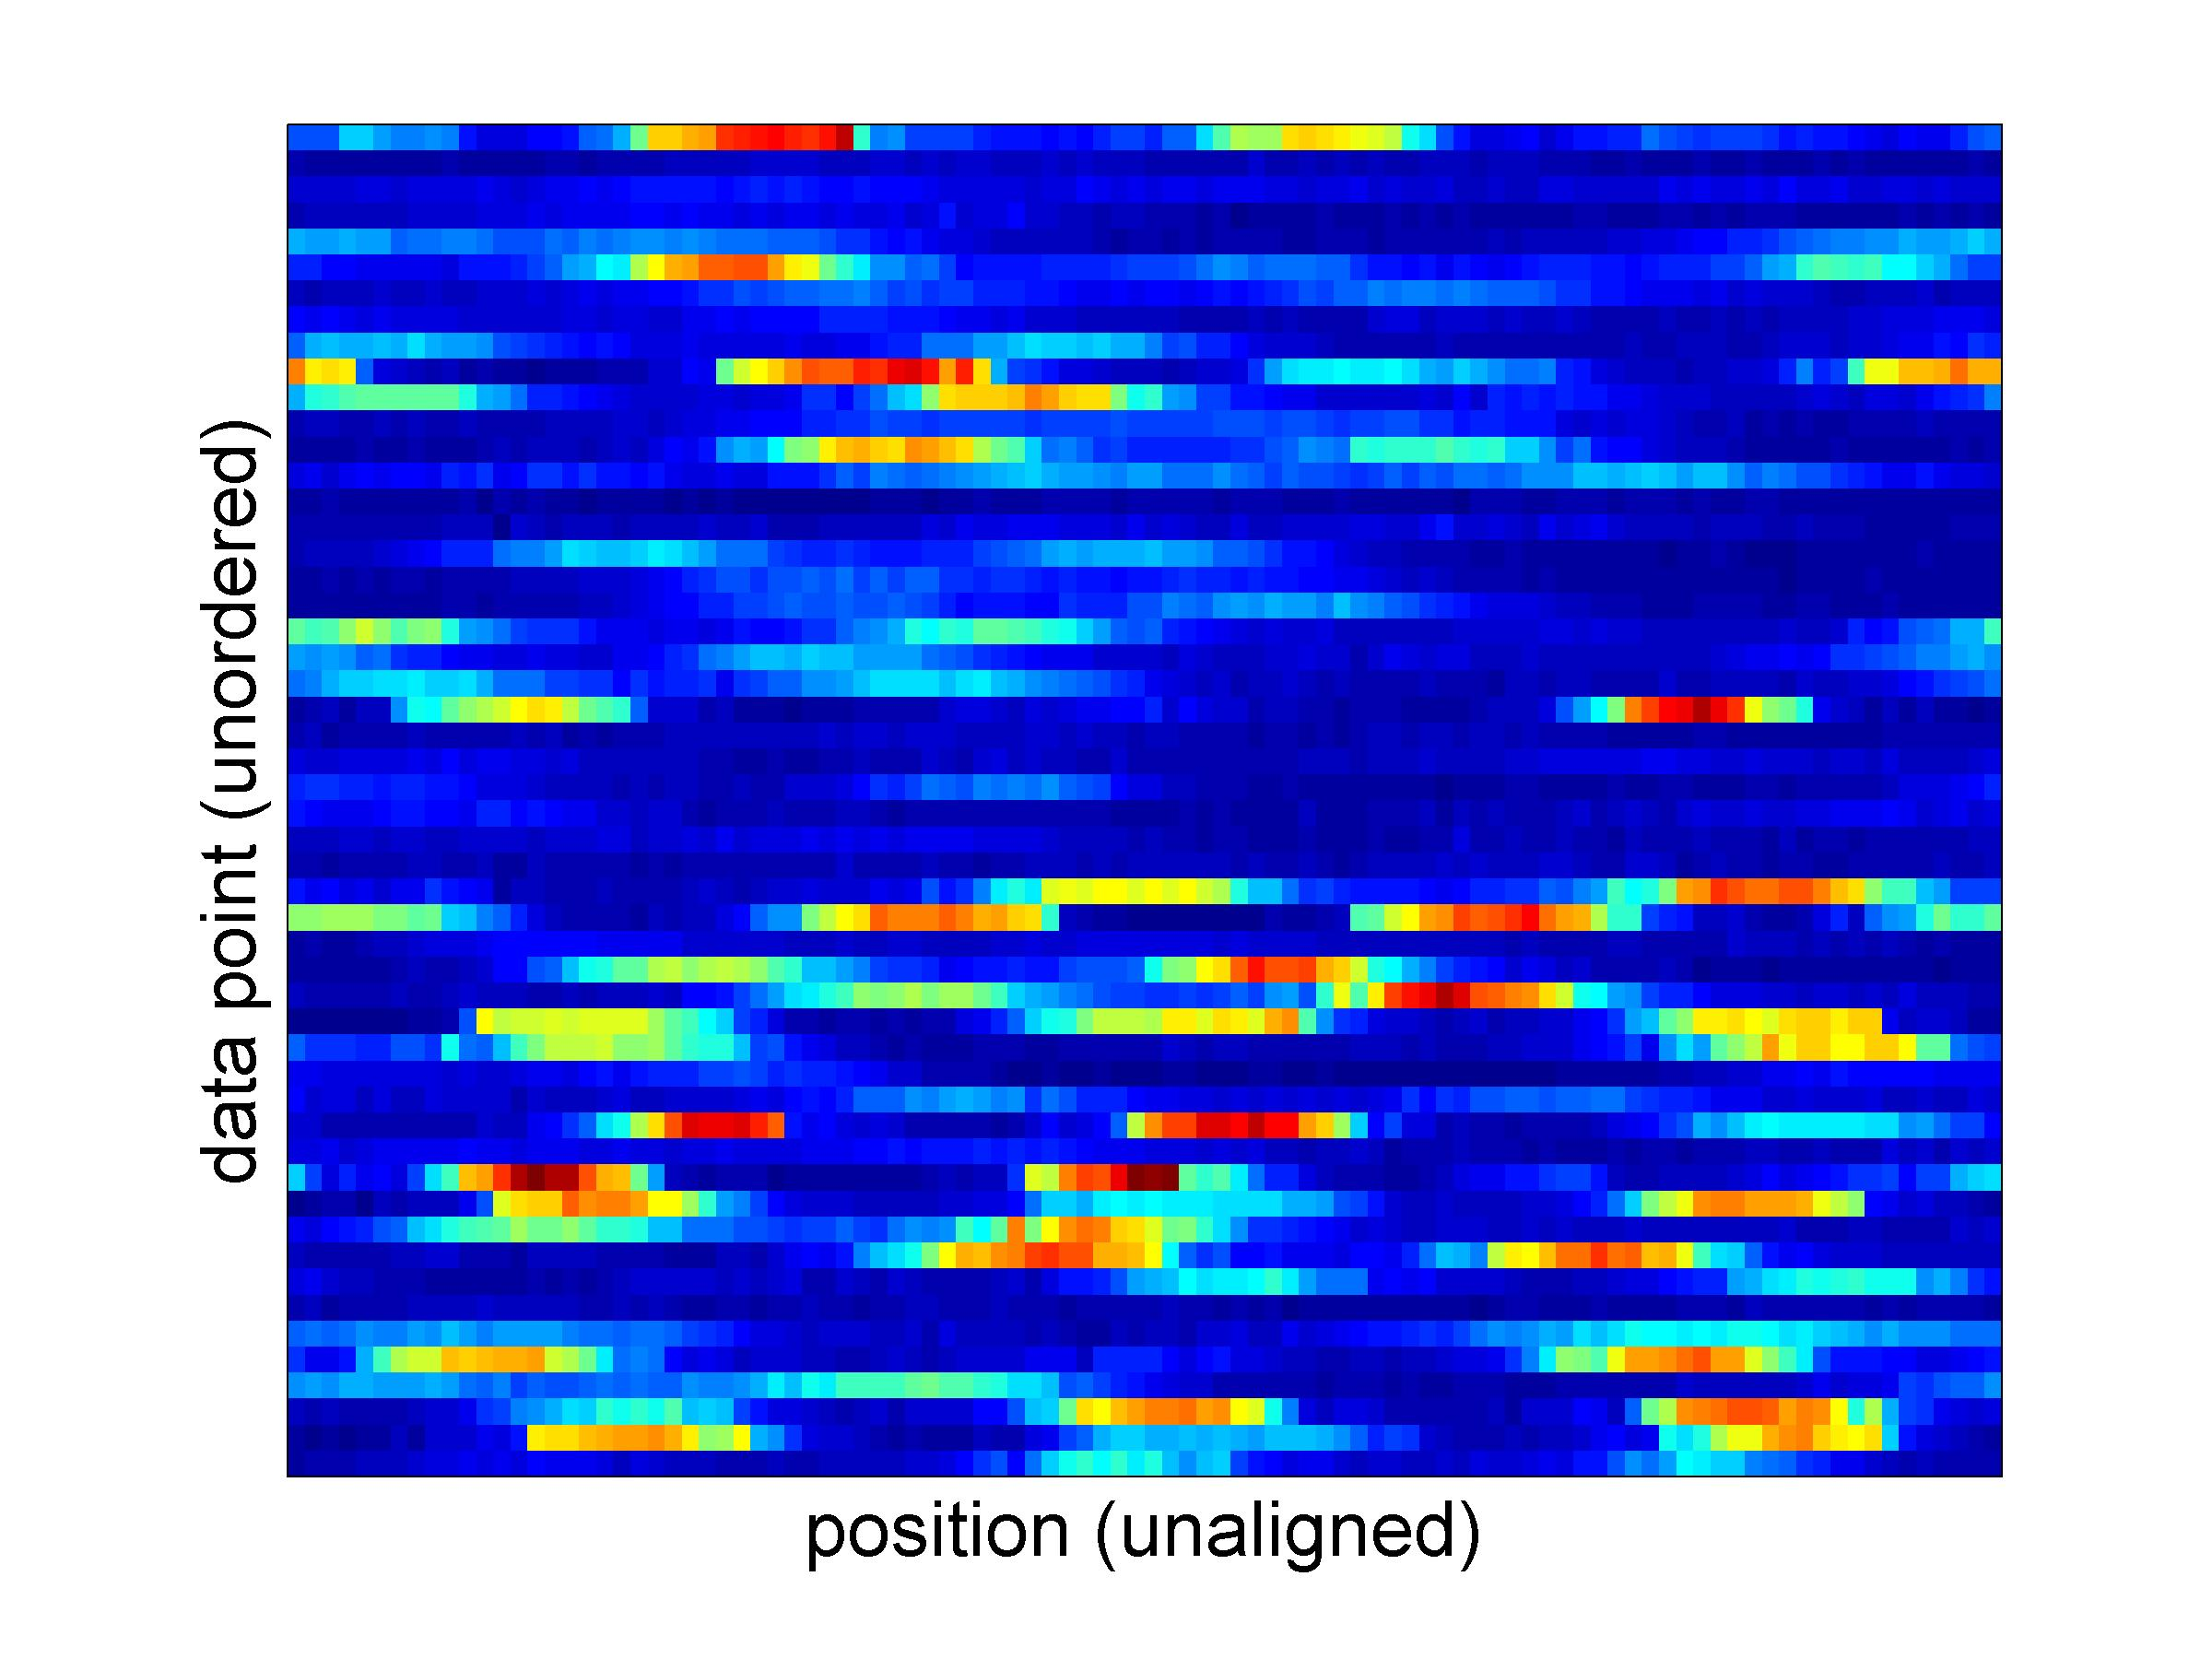
\includegraphics[width=\textwidth]{data_unaligned_unordered}
\caption{}
\end{subfigure}
\begin{subfigure}{0.3\textwidth}
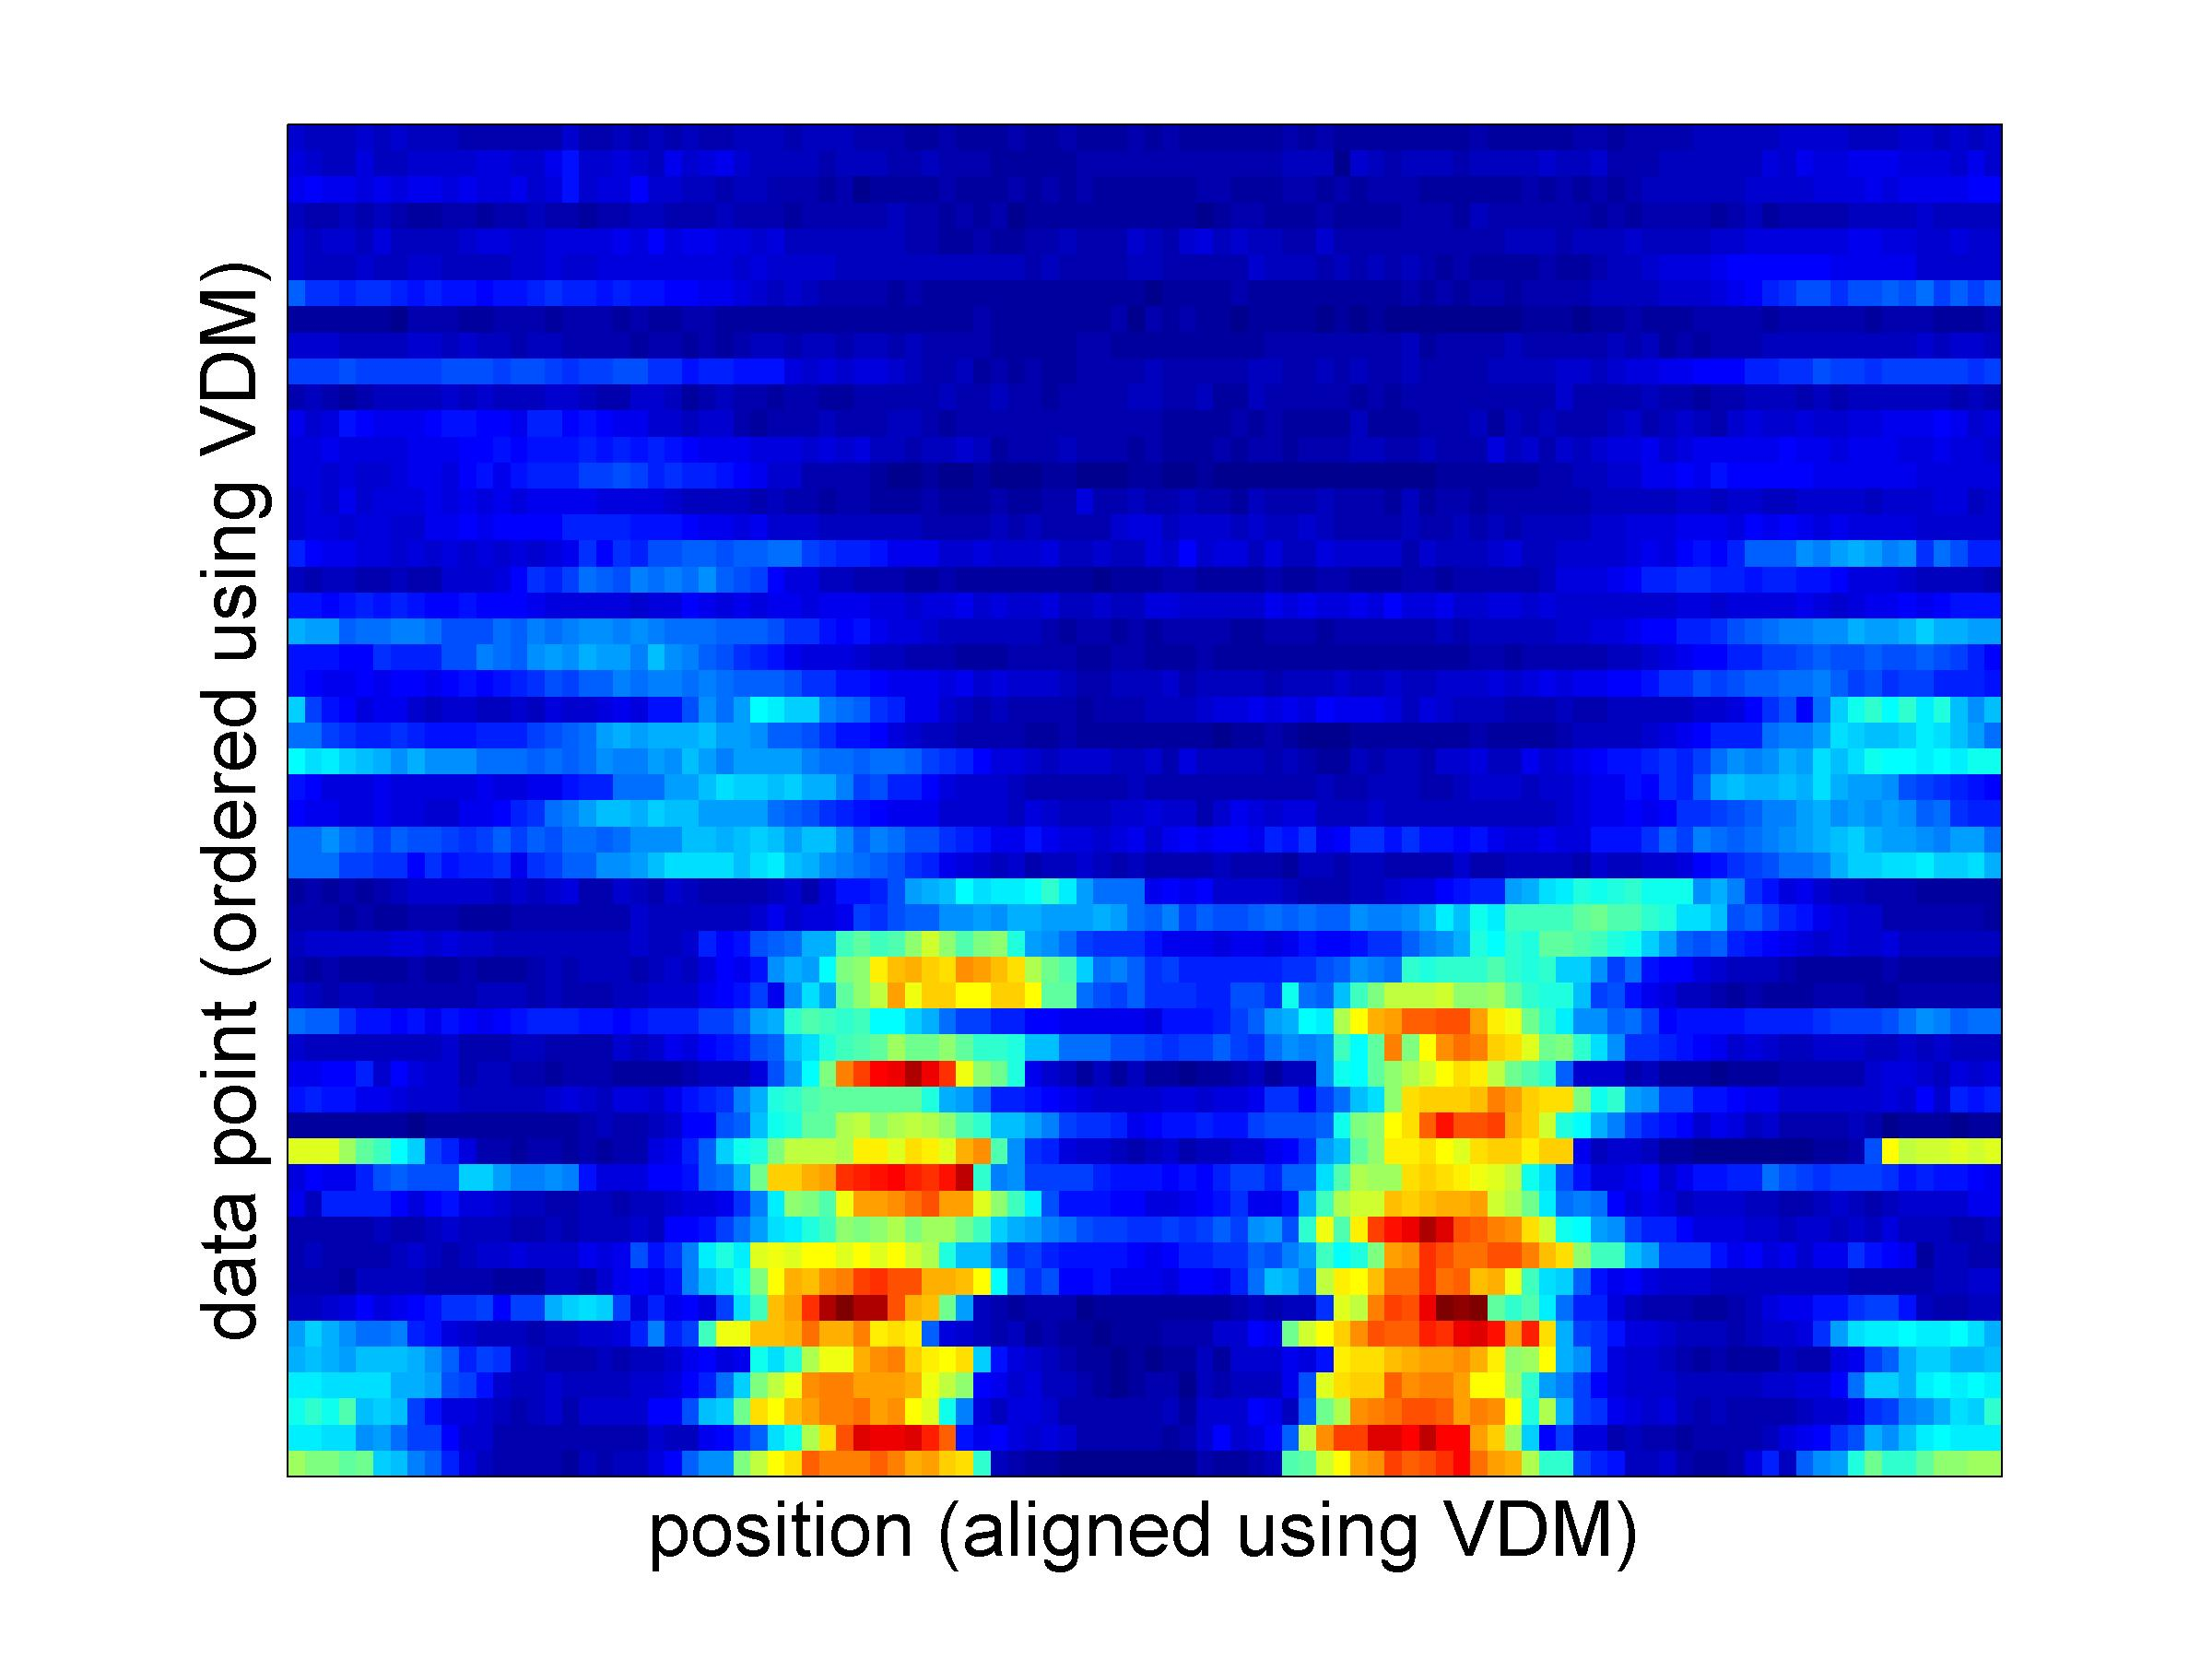
\includegraphics[width=\textwidth]{data_ordered_vdm}
\caption{}
\end{subfigure}
\begin{subfigure}{0.3\textwidth}
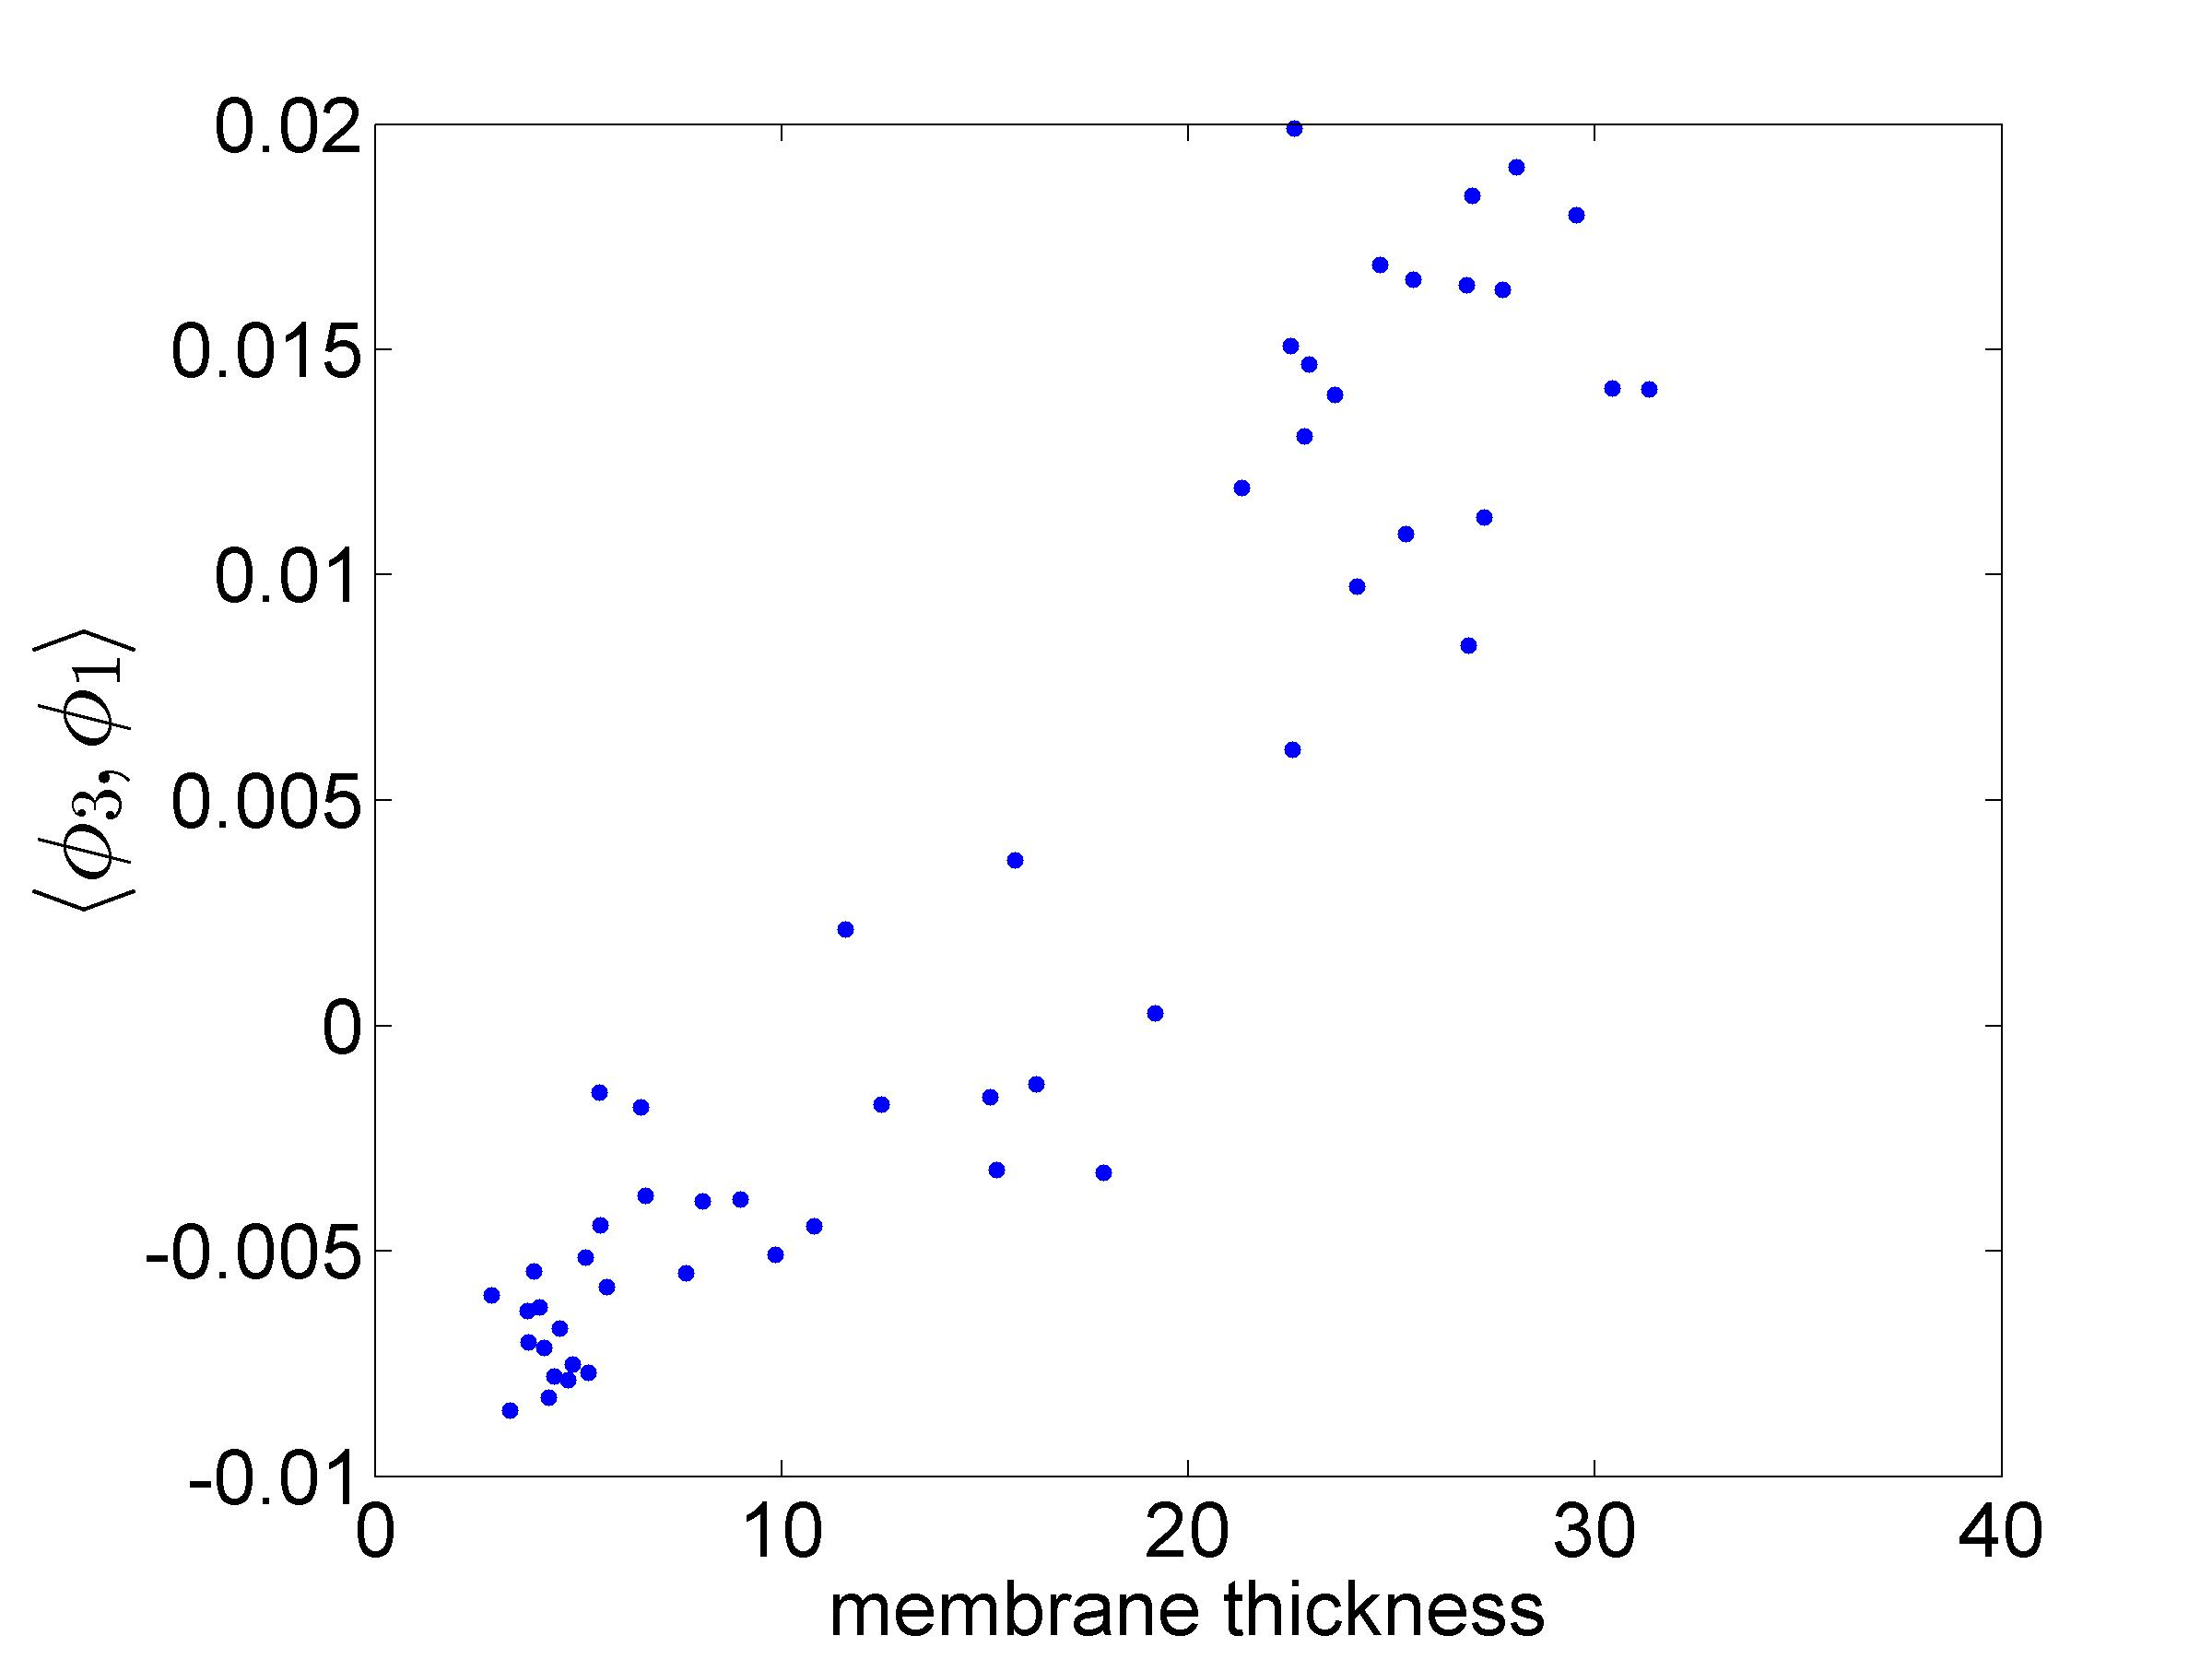
\includegraphics[width=\textwidth]{VDM_time_corr}
\caption{}
\end{subfigure}
\caption{{\bf Ordering spatially unaligned dpERK concentration profiles using vector diffusion maps.} (a) Concentration profiles of dpERK for many embryos. Each row represents a different embryo fixed at a slightly different developmental time. The circluar profiles have not been ``opened'' at the same point; rather, each profile was opened at a random point around the embryo. We are allowed to shift the (linear) profiles left and right.
(b) Concentration profiles of dpERK aligned and ordered using vector diffusion maps.
(c) Correlation between the VDM embedding coordinate and the membrane thickness.}
\label{fig:vdm_ordering}
\end{figure}

\subsection*{Two-dimensional dpERK images aligned and ordered using vector diffusion maps}

\begin{figure}[H]
\centering
\begin{subfigure}{0.45\textwidth}
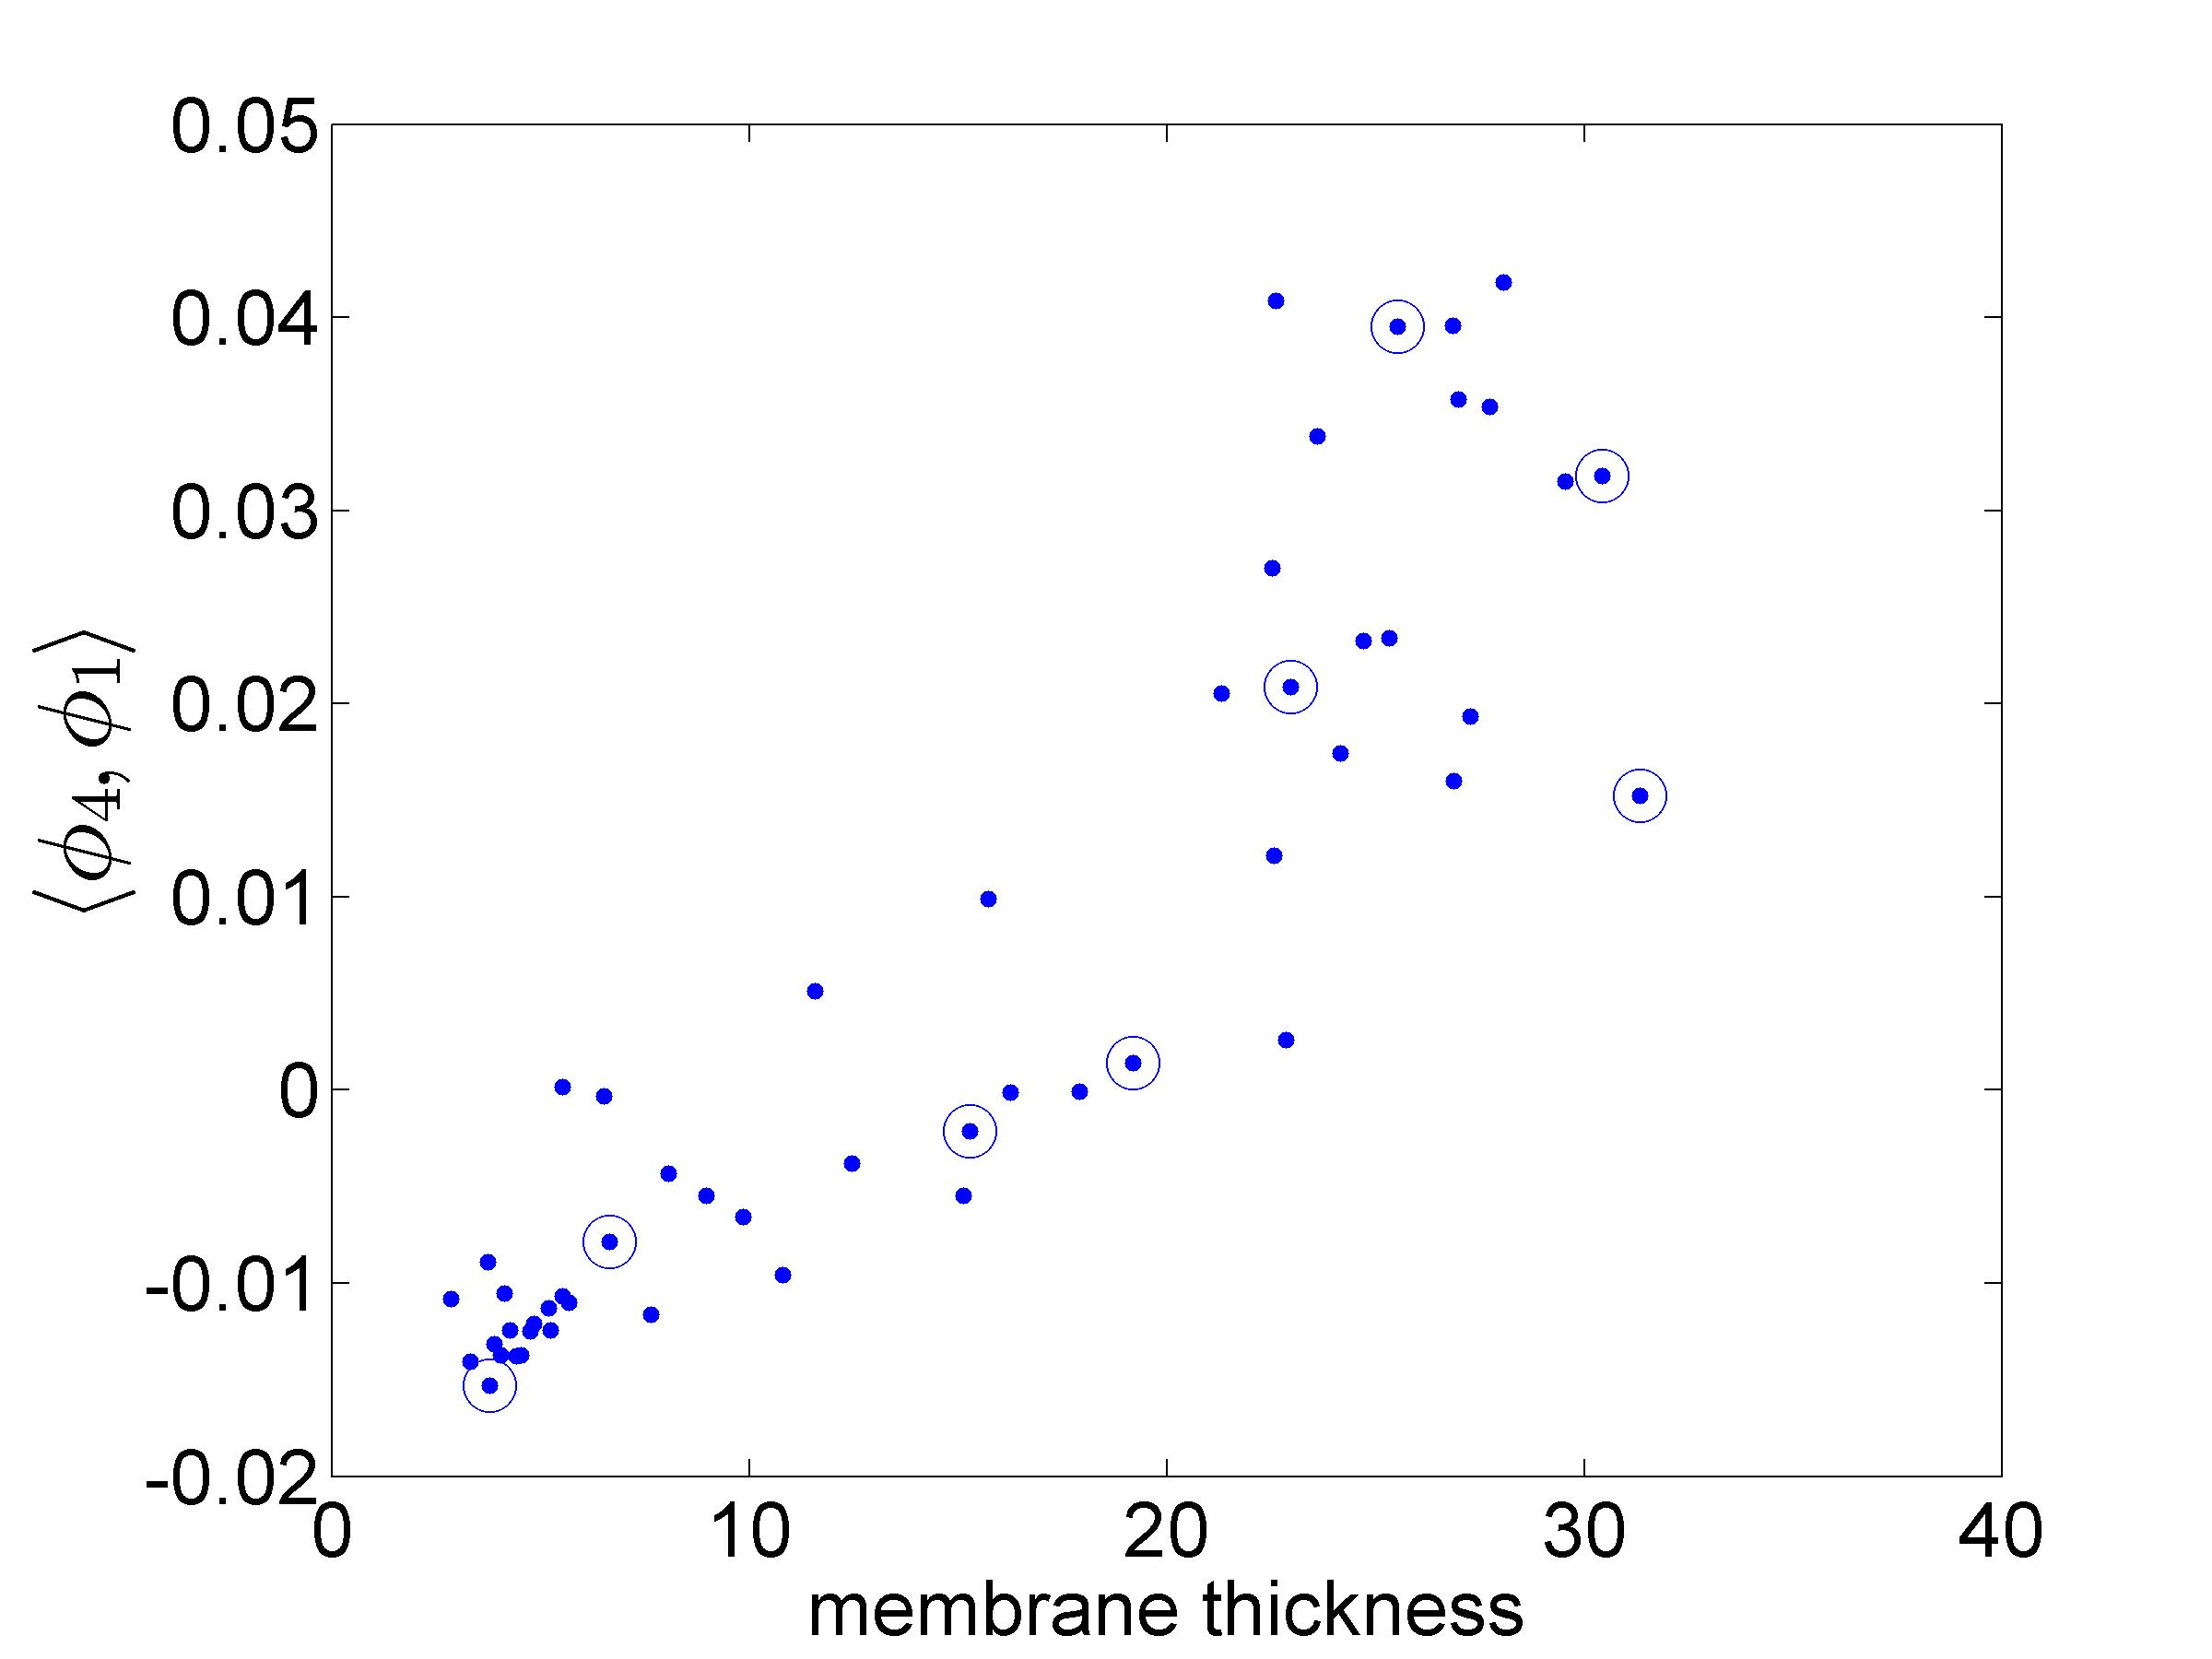
\includegraphics[width=\textwidth]{vdm_2d_time_corr}
\caption{}
\end{subfigure}
\begin{subfigure}{0.5\textwidth}
\foreach \n in {1,9,17,25,30,34,38,43,49}{
\includegraphics[width=0.3\textwidth]{dpERK_vdm_\n}
\hfill}
\caption{}
\end{subfigure}
\caption{{\bf Ordering two-dimensional fluorescent images of dpERK.}
(a) Correlation between the VDM embedding coordinate and the membrane thickness. 
(b) Some representative fluorescent images, aligned  and ordered using the VDM embedding coordinate. }
\label{fig:vdm_image_ordering}
\end{figure}

\subsection*{Two-dimensional dpERK images ordered using diffusion maps and the scattering transform}

\begin{figure}[H]
\centering
\begin{subfigure}{0.45\textwidth}
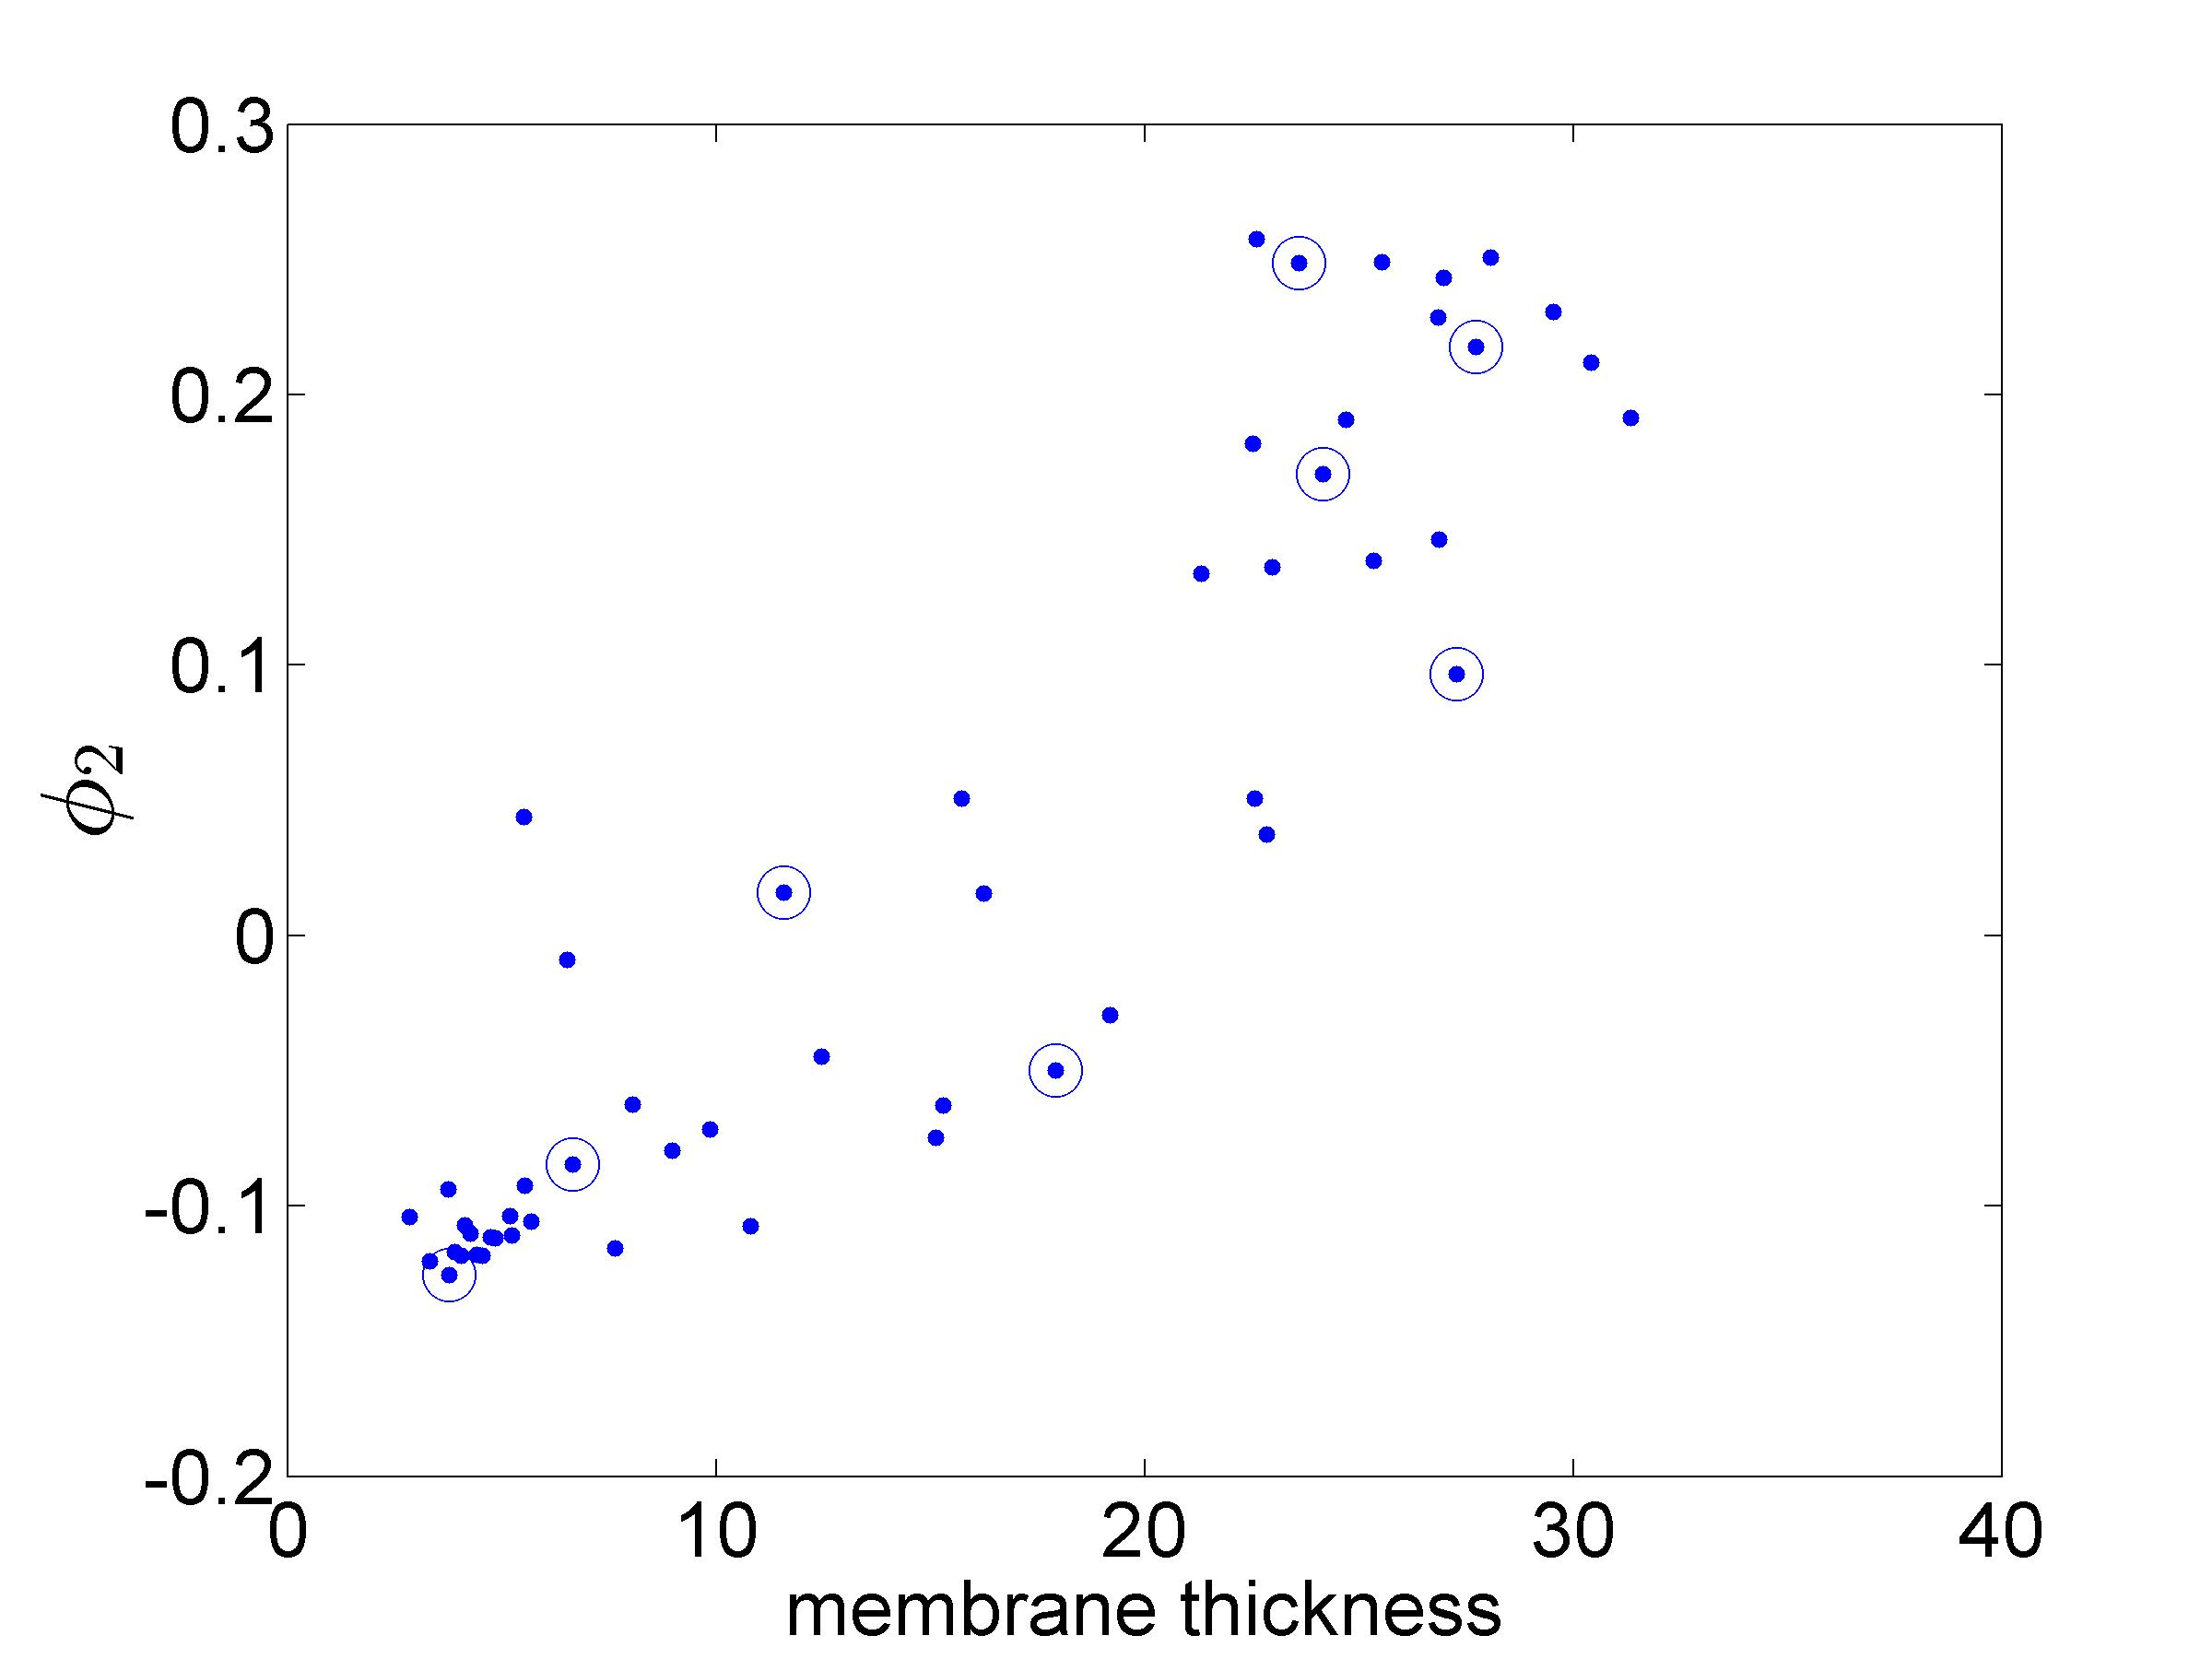
\includegraphics[width=\textwidth]{DMAPS_scat_time_corr}
\caption{}
\end{subfigure}
\begin{subfigure}{0.5\textwidth}
\foreach \n in {1,9,17,25,30,34,38,43,49}{
\includegraphics[width=0.3\textwidth]{dpERK_scat_\n}
\hfill}
\caption{}
\end{subfigure}
\caption{{\bf Ordering two-dimensional fluorescent images of dpERK.}
(a) Correlation between the first (non-trivial) DMAPS embedding coordinate and the membrane thickness. The DMAPS embedding was computed using the translation- and rotation-invariant scattering transform coefficients as ``features'' of the images.
(b) Some representative fluorescent images, ordered using the first (non-trivial) DMAPS embedding coordinate computed from the scattering transform coefficients. }
\label{fig:scattrans_dpERK_ordering}
\end{figure}

\subsection*{Two-dimensional membrane images ordered using diffusion maps and the scattering transform}

\begin{figure}[H]
\centering
\begin{subfigure}{0.45\textwidth}
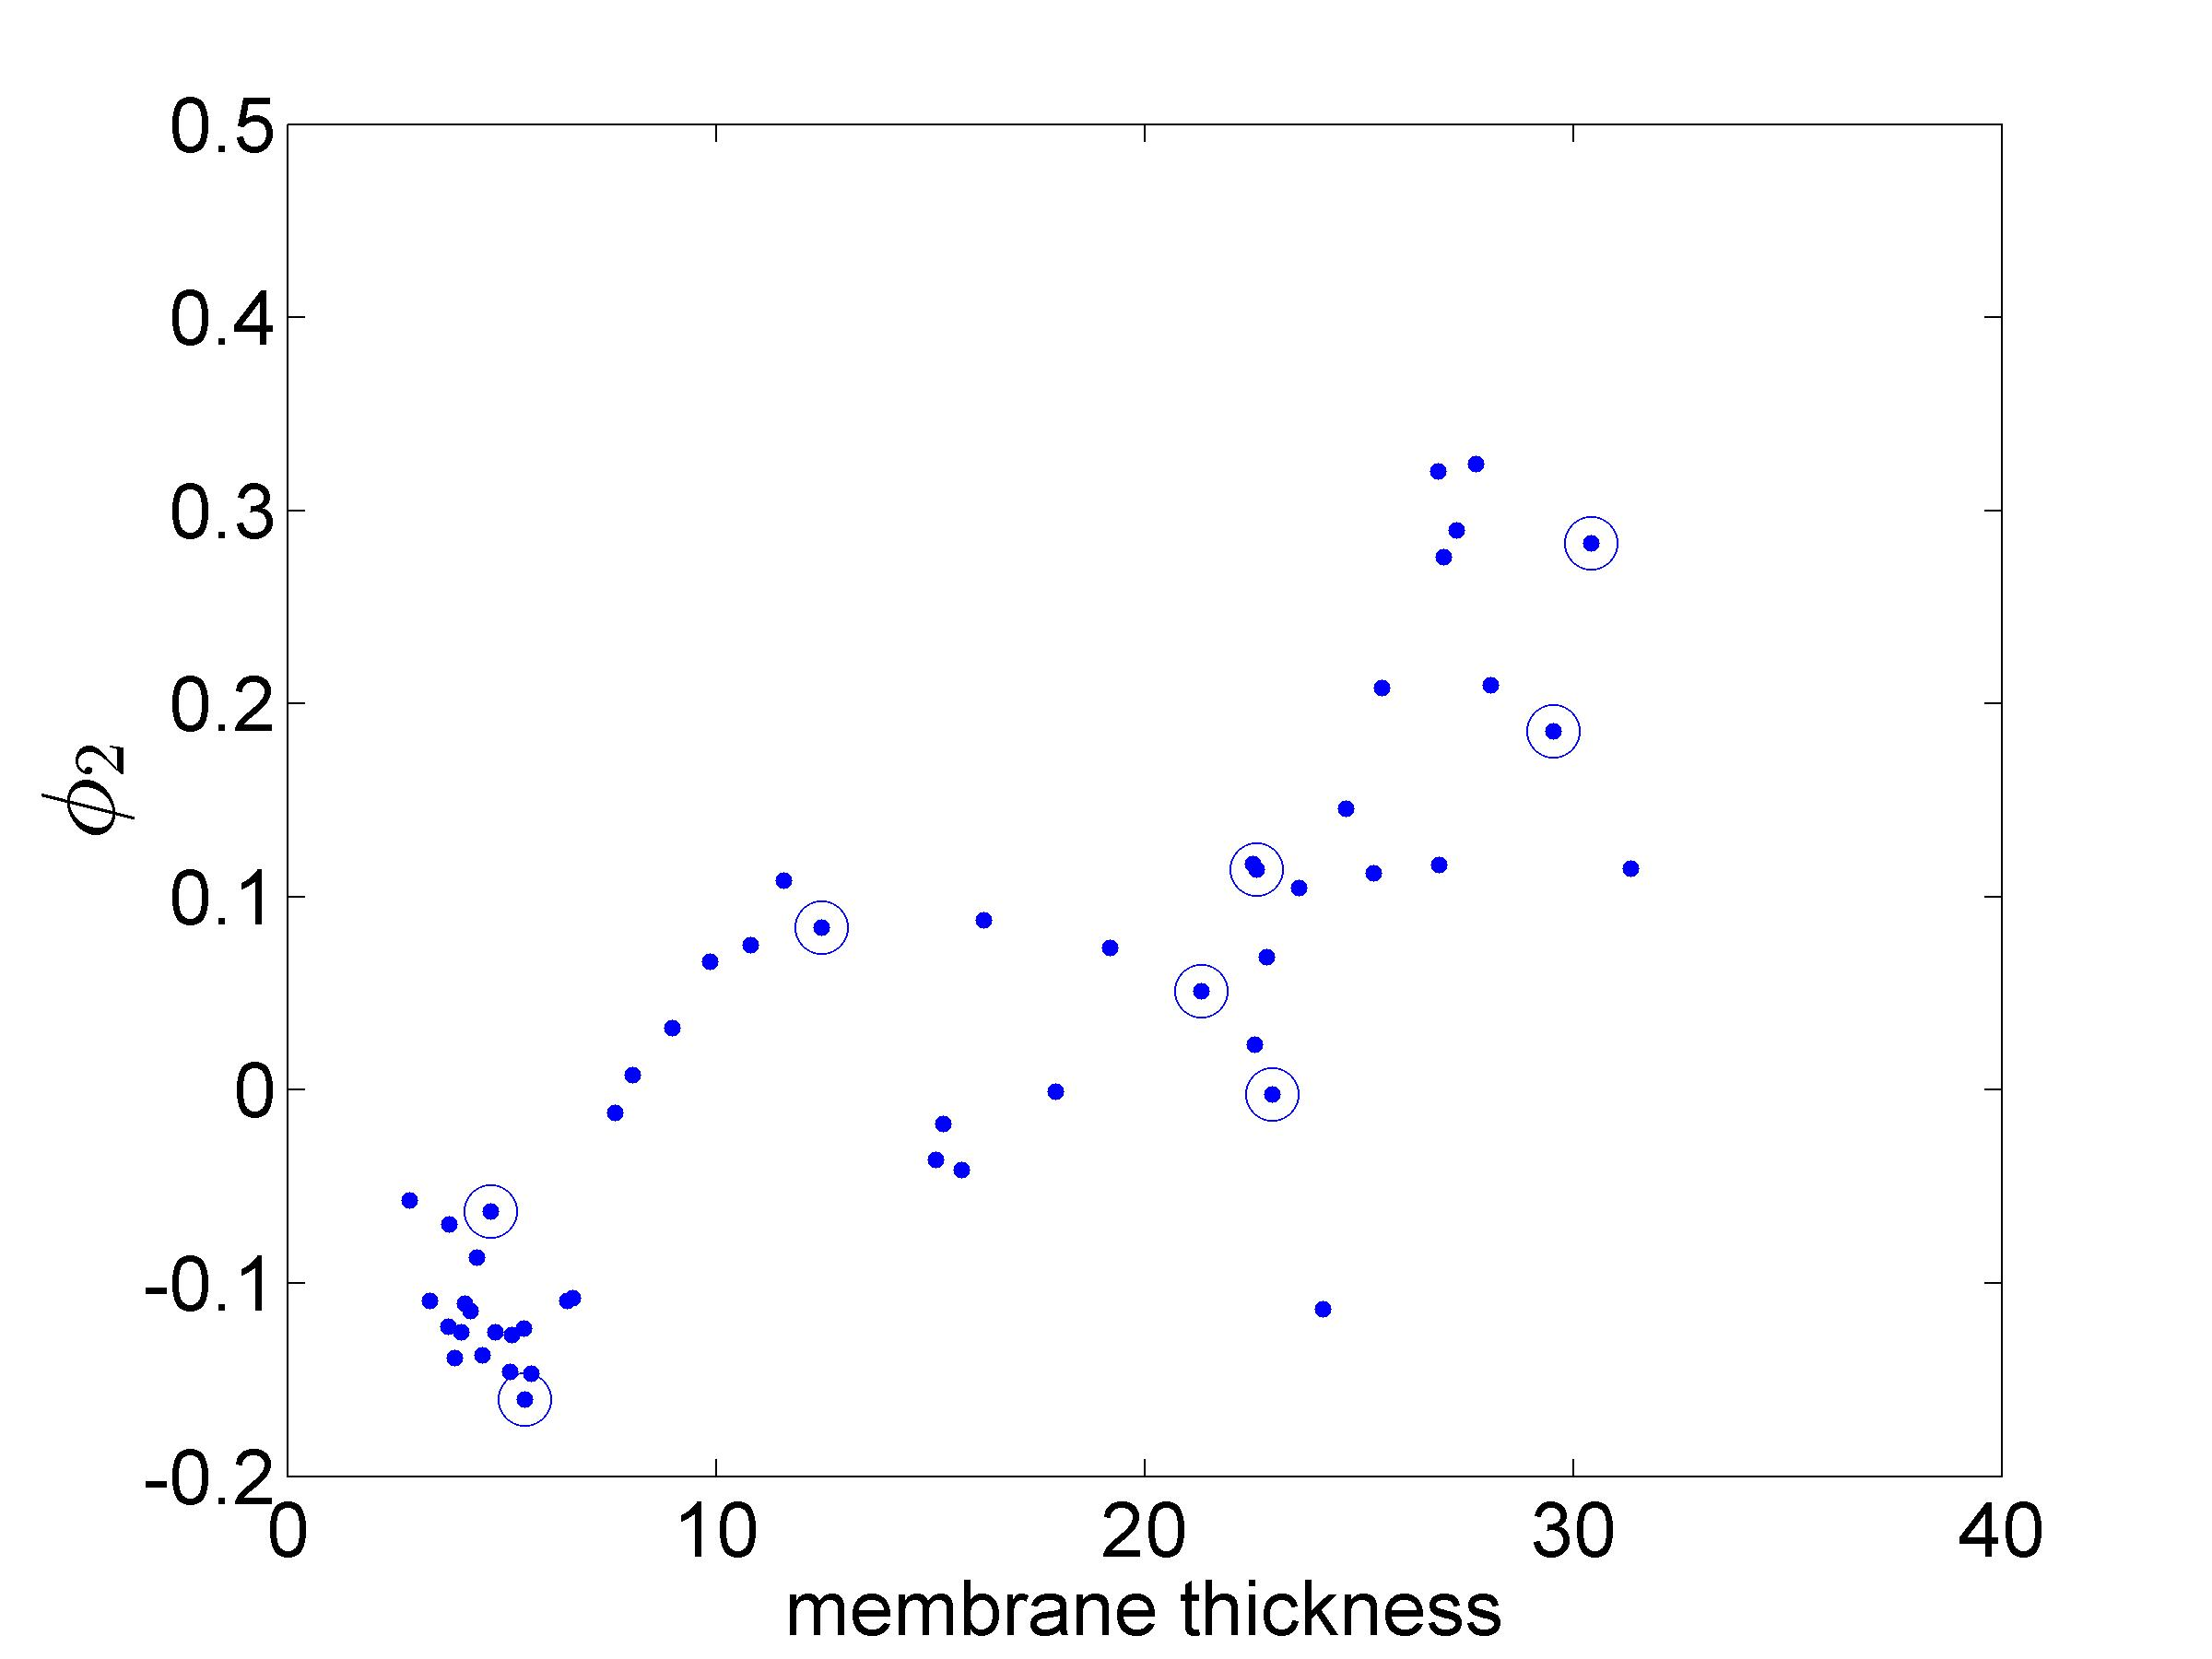
\includegraphics[width=\textwidth]{DMAPS_membrane_scat_time_corr}
\caption{}
\end{subfigure}
\begin{subfigure}{0.5\textwidth}
\foreach \n in {1,9,17,25,30,34,38,43,49}{
\includegraphics[width=0.3\textwidth]{membrane_scat_\n}
\hfill}
\caption{}
\end{subfigure}
\caption{{\bf Ordering two-dimensional fluorescent images of membrane proteins.}
(a) Correlation between the seventh (non-trivial) DMAPS embedding coordinate and the membrane thickness. DMAPS was computed using the translation- and rotation-invariant scattering transform coefficients as ``features'' of the images. The first six non-trivial DMAPS coordinates were found to capture other features of the images, such as  differences in fluorescence intensity within the images.
(b) Some representative fluorescent images, ordered using the seventh (non-trivial) DMAPS embedding coordinate computed from the scattering transform coefficients. }
\label{fig:scattrans_membrane_ordering}
\end{figure}


\section*{Discussion}

% You may title this section "Methods" or "Models".
% "Models" is not a valid title for PLoS ONE authors. However, PLoS ONE
% authors may use "Analysis"
\section*{Materials and Methods}

\subsection*{Experimental Setup}

\subsection*{Principal Component Analysis}
Principal component analysis, or PCA, has been the workhorse dimensionality reduction technique for the past century.
%
PCA finds the optimal planes or hyperplanes on which to project the data in order to maximize the variance of the projected data.

We assume we have a data set consisting of $n$ $d$-dimensional observations, $X \in \mathbb{R}^{n \times d}$, where $X_{ij}$ denotes the $j^{th}$ dimension of the $i^{th}$ observation. 
%
PCA first begins by mean-centering the data set to produce the matrix $\hat{X}$, where
\begin{equation}
\hat{X}_{ij} = X_{ij} - \frac{1}{n} \sum_{k=1}^n X_{kj}.
\end{equation}
%
The empirical covariance of the data set, $C \in mathbb{R}^{d \times d}$ can be computed as
\begin{equation}
C = X^T X.
\end{equation}
%
The principal components of the data set $X$ are then given by the eigenvectors $\psi_1, \dots, \psi_d$ of $C$.
%
Furthermore, the eigenvalues $\lambda_1, \lambda_2, \dots, \lambda_d$ measure the variance of the data capatured by the corresponding eigenvector. 
%
Therefore, we choose to order the eigenvectors such that $\lambda_1 \ge \lambda_2 \ge \dots \ge \lambda_d$.
%
Then, the first few eigenvectors capture a significant portion of the variance in our data set, and projection onto these first few principal components will retain many features of the data set while reducing the dimenstionality.
%
In our setup, we assume that the data is inherently one-dimensional, and that projection onto $\psi_1$ will uncover the correct time ordering of the data.

\subsection*{Diffusion Maps}
Unlike PCA, diffusion maps (DMAPS) is a nonlinear dimensionality reduction technique. 
%
DMAPS aims to uncover the parameterization of data sampled from a nonlinear manifold.
%
The {\em essential} requirement for DMAPS is an appropriate distance metric $d(x_i, x_j)$ for comparing data points. 
%
This can be the standard Euclidean distance, or a more complex metric for other data sets.

We then calculate the matrix $W \in \mathbb{R}^{n \times n}$, where 
\begin{equation}
W_{ij} = \exp \left( -\frac{d^2(x_i, x)j)}{\epsilon} \right)
\end{equation}
and $\epsilon$ is a characteristic distance between data points.
%
In practice, we choose $\epsilon$ to be the median of the pairwise distances between data points.
%
We then compute the diagonal matrix $D$, where $D_{ii} = \sum_{j=1}^{n} W_{ij}$, and the matrix $A = D^{-1} W$. 
%
We then compute the eigenvectors $\phi_1, \phi_2, \dots, \phi_n$ and eigenvalues $\lambda_1, \lambda_2, \dots, \lambda_n$ and order them such that $|\lambda_1| \ge |\lambda_2| \ge \dots \ge |\lambda_n|$. 
%


\subsection*{Angular Synchronization}

\subsection*{Vector Diffusion Maps} 

\subsection*{Scattering Transform}

% Do NOT remove this, even if you are not including acknowledgments
\section*{Acknowledgments}


%\section*{References}
% The bibtex filename
\bibliography{template}

\section*{Figure Legends}
%\begin{figure}[!ht]
%\begin{center}
%%\includegraphics[width=4in]{figure_name.2.eps}
%\end{center}
%\caption{
%{\bf Bold the first sentence.}  Rest of figure 2  caption.  Caption
%should be left justified, as specified by the options to the caption
%package.
%}
%\label{Figure_label}
%\end{figure}


\section*{Tables}
%\begin{table}[!ht]
%\caption{
%\bf{Table title}}
%\begin{tabular}{|c|c|c|}
%table information
%\end{tabular}
%\begin{flushleft}Table caption
%\end{flushleft}
%\label{tab:label}
% \end{table}

\end{document}
